\documentclass[a4paper, 12pt]{extreport}

\usepackage[T2A]{fontenc}
\usepackage[utf8]{inputenc}
\usepackage[english,russian]{babel}
\usepackage{amssymb,amsfonts,amsmath,mathtext,cite,enumerate,float}
\usepackage{pgfplots}
\usepackage{tikz}
\usetikzlibrary{shapes.geometric, arrows, positioning, calc, er, shadows, decorations.pathreplacing, shapes.multipart, fit}
\usepackage{graphicx}
\usepackage{tocloft}
\usepackage{listings}
\usepackage{caption}
\usepackage{tempora}
\usepackage{titlesec}
\usepackage{tabularx}
\usepackage{setspace}
\usepackage{geometry}
\usepackage{indentfirst}
\usepackage{pdfpages}
\usepackage{enumerate,letltxmacro}
\usepackage{threeparttable}
\usepackage[breaklinks=true]{hyperref}
\usepackage{flafter}
\usepackage{enumitem}
\usepackage{multirow}
\usepackage{array}
\usepackage{ragged2e}

% Компактные таблицы (имена типов не с «C», чтобы не конфликтовать с array)
\newcolumntype{Y}[1]{>{\RaggedRight\arraybackslash}p{#1}}
\newcolumntype{Z}[1]{>{\ttfamily\footnotesize\RaggedRight\arraybackslash}p{#1}}

\usepackage[figure,table]{totalcount}
\usepackage{lastpage}

\setlist{nosep}

\newcommand{\ssr}[1]{\begin{center}
		\LARGE\bfseries{#1}
	\end{center} \addcontentsline{toc}{chapter}{#1}  }

\makeatletter
\renewcommand\LARGE{\@setfontsize\LARGE{22pt}{20}}
\renewcommand\Large{\@setfontsize\Large{20pt}{20}}
\renewcommand\large{\@setfontsize\large{16pt}{20}}
\makeatother
\RequirePackage{titlesec}
\titleformat{\chapter}[block]{\hspace{\parindent}\large\bfseries}{\thechapter}{0.5em}{\large\bfseries\raggedright}
\titleformat{name=\chapter,numberless}[block]{\hspace{\parindent}}{}{0pt}{\large\bfseries\centering}
\titleformat{\section}[block]{\hspace{\parindent}\large\bfseries}{\thesection}{0.5em}{\large\bfseries\raggedright}
\titleformat{\subsection}[block]{\hspace{\parindent}\large\bfseries}{\thesubsection}{0.5em}{\large\bfseries\raggedright}
\titleformat{\subsubsection}[block]{\hspace{\parindent}\large\bfseries}{\thesubsection}{0.5em}{\large\bfseries\raggedright}
\titlespacing{\chapter}{12.5mm}{-22pt}{10pt}
\titlespacing{\section}{12.5mm}{10pt}{10pt}
\titlespacing{\subsection}{12.5mm}{10pt}{10pt}
\titlespacing{\subsubsection}{12.5mm}{10pt}{10pt}

\makeatletter
\renewcommand{\@biblabel}[1]{#1.}
\makeatother

\geometry{left=30mm}
\geometry{right=10mm}
\geometry{top=20mm}
\geometry{bottom=20mm}

\onehalfspacing

\renewcommand{\theenumi}{\arabic{enumi}}
\renewcommand{\labelenumi}{\arabic{enumi})}
\renewcommand{\theenumii}{.\arabic{enumii}}
\renewcommand{\labelenumii}{\arabic{enumi}.\arabic{enumii})}
\renewcommand{\theenumiii}{.\arabic{enumiii}}
\renewcommand{\labelenumiii}{\arabic{enumi}.\arabic{enumii}.\arabic{enumiii})}

\renewcommand{\cftchapleader}{\cftdotfill{\cftdotsep}}

\addto\captionsrussian{\renewcommand{\figurename}{Рисунок}}
\DeclareCaptionLabelSeparator{dash}{~---~}
\captionsetup{labelsep=dash}

\captionsetup[figure]{justification=centering,labelsep=dash}
\captionsetup[table]{labelsep=dash,justification=raggedright,singlelinecheck=off}

\graphicspath{{images/}}

\newcommand{\floor}[1]{\lfloor #1 \rfloor}

\lstset{
 basicstyle=\ttfamily\small,
 numbers=none,
 numberstyle=\color{black}\ttfamily\small,
 stepnumber=1,
 numbersep=10pt,
 frame=single,
 tabsize=2,
 captionpos=t,
 breaklines=true,
 breakatwhitespace=false,
 escapeinside={\#*}{*)},
 columns=fixed,
 keepspaces=true,
 showstringspaces=false,
 showtabs=false,
 xleftmargin=25pt,
 framexleftmargin=20pt
}

\pgfplotsset{compat=1.18, width=0.85\linewidth, height=0.5\columnwidth}

\linespread{1.3}

\parindent=1.25cm

\def\labelitemi{---}
\setlist[itemize]{leftmargin=1.25cm, itemindent=0.65cm}
\setlist[enumerate]{leftmargin=1.25cm, itemindent=0.55cm}

\newcommand{\specialcell}[2][c]{%
	\begin{tabular}[#1]{@{}c@{}}#2\end{tabular}}

\frenchspacing


\begin{document}
	
\includepdf[pages=1]{title.pdf}
	\setcounter{page}{2}

	% Остальные разделы курсовой (введение, конструкторский, технологический,
	% исследовательский, заключение, список литературы, приложения) --- по мере подготовки.

	\chapter*{РЕФЕРАТ}
\addcontentsline{toc}{chapter}{РЕФЕРАТ}

РПЗ содержит 65~с., 18~рис., 30~табл., 7~приложений, 23~источника.

Ключевые слова: база данных, спортивная аналитика, NBA, реляционная
модель, \newline PostgreSQL, Redis, кэширование, метрики эффективности, PER, BPM,
REST API, ролевая модель, индексация, производительность.

Объект исследования~--- процессы накопления, обработки и анализа
массивов спортивной статистики NBA.

Предмет исследования~--- структура базы данных
и алгоритмы вычисления комплексных показателей эффективности баскетболистов.

Цель работы~--- разработка базы данных для хранения и анализа
статистики игроков и команд Национальной баскетбольной ассоциации
с реализацией автоматизированных расчётов комплексных показателей эффективности.

В аналитическом разделе проведён сравнительный анализ существующих систем
спортивной статистики, сформулированы функциональные и нефункциональные
требования, формализованы правила расчёта пяти комплексных показателей
(TS\%, eFG\%, USG\%, PER, BPM), выделены восемь сущностей предметной
области, построены ER-диаграмма и диаграмма вариантов использования,
обоснован выбор реляционной модели данных со строковым хранением.

В конструкторском разделе спроектирована реляционная схема из восьми
таблиц, трёх представлений и шести индексов, доказано соответствие 3НФ,
разработаны алгоритмы расчёта метрик и ограничений целостности
(схемы алгоритмов приведены в приложении~А), определена ролевая модель из трёх ролей,
спроектировано REST API из 20~маршрутов и механизм кэширования по паттерну Cache-Aside.

В технологическом разделе обоснован выбор стека (PostgreSQL~15, Redis~7,
FastAPI, React~18), реализована физическая структура базы данных,
разработаны хранимые PL/pgSQL-функции и триггеры (приложение~Г),
приведены примеры SQL-запросов (приложение~В), база данных наполнена
реальной статистикой NBA объёмом более 150\,000 фактов, реализован
пользовательский интерфейс (приложение~Е), проведено регрессионное
тестирование с верификацией по классам эквивалентности.

В исследовательском разделе измерено влияние стратегий индексации,
предвычисленной витрины и кэширования Redis на производительность
аналитических запросов; проведено нагрузочное тестирование
при конкурентном доступе до 100~одновременных подключений;
сформулированы рекомендации по оптимизации.

Разработанный программный комплекс применим в качестве аналитической
платформы для профильных специалистов спортивных организаций.


	\clearpage
	\begin{center}
		\LARGE\bfseries\MakeUppercase{СОДЕРЖАНИЕ}
	\end{center}
	\vspace*{-31mm}
	\begingroup
	\let\contentsname\relax
	\tableofcontents
	\endgroup

	\ssr{СПИСОК ИСПОЛЬЗУЕМЫХ СОКРАЩЕНИЙ И ОБОЗНАЧЕНИЙ}

\subsection*{Спортивные метрики и обозначения}

\noindent
\begin{tabular}{@{}>{\bfseries}p{2.6cm}Y{12.7cm}@{}}
AST   & передачи (assists) \\
BLK   & блок-шоты (blocks) \\
BPM   & вклад игрока (Box Plus/Minus) \\
eFG\% & эффективный процент с игры (effective field goal percentage) \\
FG3A  & попытки трёхочкового броска \\
FG3M  & попадания трёхочковых бросков \\
FGA   & попытки броска с игры (field goals attempted) \\
FGM   & попадания с игры (field goals made) \\
FTA   & попытки штрафного броска (free throws attempted) \\
FTM   & попадания штрафных бросков (free throws made) \\
MP    & минуты на площадке (minutes played) \\
NBA   & Национальная баскетбольная ассоциация \\
PER   & рейтинг эффективности игрока (Player Efficiency Rating) \\
PF    & персональные фолы (personal fouls) \\
PTS   & очки (points) \\
REB\_DEF & подборы в защите \\
REB\_OFF & подборы в нападении \\
STL   & перехваты (steals) \\
TmFGA & командные попытки броска с игры \\
TmFTA & командные попытки штрафного броска \\
TmMP  & суммарные минуты команды \\
TmTOV & командные потери \\
TOV   & потери (turnovers) \\
TRB   & подборы суммарные (total rebounds) \\
TS\%  & истинный процент бросков (true shooting percentage) \\
USG\% & доля владений в атаке (usage percentage) \\
\end{tabular}

\subsection*{Технические}

\noindent
\begin{tabular}{@{}>{\bfseries}p{2.6cm}Y{12.7cm}@{}}
ACID      & Atomicity, Consistency, Isolation, Durability \\
API       & Application Programming Interface \\
ASGI      & Asynchronous Server Gateway Interface \\
B-tree    & сбалансированное дерево (balanced tree) \\
CORS      & Cross-Origin Resource Sharing \\
CRUD      & Create, Read, Update, Delete \\
DDL       & Data Definition Language \\
ER        & Entity-Relationship \\
ETL       & Extract, Transform, Load \\
FK        & внешний ключ (Foreign Key) \\
HTAP      & Hybrid Transactional/Analytical Processing \\
HTTP      & Hypertext Transfer Protocol \\
JSON      & JavaScript Object Notation \\
KPI       & ключевые показатели эффективности (Key Performance Indicators) \\
OLAP      & Online Analytical Processing \\
OLTP      & Online Transaction Processing \\
P95       & 95-й перцентиль \\
PK        & первичный ключ (Primary Key) \\
PL/pgSQL  & процедурный язык PostgreSQL \\
REST      & Representational State Transfer \\
SPA       & одностраничное приложение (Single Page Application) \\
SQL       & Structured Query Language \\
СУБД      & система управления базами данных \\
UML       & Unified Modeling Language \\
URL       & Uniform Resource Locator \\
UPSERT    & операция вставки с обновлением (UPDATE + INSERT) \\
1НФ / 2НФ / 3НФ & первая / вторая / третья нормальная форма \\
\end{tabular}

	\chapter*{ВВЕДЕНИЕ}
\addcontentsline{toc}{chapter}{ВВЕДЕНИЕ}

В современном профессиональном спорте, и в частности в баскетболе (Национальная баскетбольная ассоциация --- NBA), сбор и анализ статистических данных играет ключевую роль. Если ранее оценка эффективности игроков базировалась преимущественно на базовых показателях (очки, подборы, передачи), то сегодня клубы, аналитики и скауты опираются на продвинутые метрики (Advanced Stats), такие как рейтинг эффективности игрока (PER), истинный процент попаданий (TS\%) или показатель полезности (BPM). 

Обработка таких данных требует надежных и производительных систем хранения, способных не только хранить огромные массивы исторических данных по каждому матчу, но и быстро агрегировать их по сезонам, командам и игрокам. В связи с этим, проектирование оптимизированной реляционной базы данных с механизмами кэширования является актуальной задачей.

\textbf{Целью курсовой работы} является разработка базы данных и программного обеспечения для анализа статистики игроков и команд NBA с реализацией расчетных метрик эффективности.

Для достижения поставленной цели необходимо решить следующие \textbf{задачи}:
\begin{enumerate}
	\item Провести анализ предметной области и существующих систем сбора спортивной статистики.
	\item Спроектировать структуру базы данных, нормализованную до третьей нормальной формы (3НФ), и определить ограничения целостности.
	\item Разработать алгоритмы расчета продвинутых метрик результативности на стороне СУБД.
	\item Разработать ролевую модель с разграничением прав доступа к данным.
	\item Спроектировать и реализовать клиент-серверное программное обеспечение для взаимодействия с базой данных.
	\item Интегрировать механизм кэширования результатов аналитических запросов.
	\item Провести исследование влияния стратегий индексации и кэширования на производительность системы при различных уровнях нагрузки.
\end{enumerate}

\textbf{Объектом исследования} выступают системы хранения и обработки спортивной статистики.

\textbf{Предметом исследования} являются методы проектирования реляционных баз данных, оптимизации аналитических запросов и кэширования данных.

	\chapter{Аналитический раздел}

\section{Анализ предметной области}

Национальная баскетбольная ассоциация (NBA) является источником одного из наиболее
детализированных массивов спортивной статистики среди крупнейших мировых
профессиональных лиг~\cite{nba-stats}. Для каждого матча фиксируются итоговый
счёт, составы команд и числовые показатели по каждому игроку: очки, подборы,
передачи, блок-шоты, перехваты и иные. На этой основе можно строить рейтинги,
сопоставлять сезоны и выявлять тенденции развития игры.

В современной баскетбольной аналитике для комплексной оценки результативности применяются
продвинутые метрики, стандартизированные в работах ведущих спортивных статистиков~\cite{kubatko}.
Расчёт таких показателей как истинный процент бросков TS\%, эффективный процент с игры eFG\%,
доля владений в атаке USG\%, рейтинг эффективности игрока PER и показатель вклада
игрока BPM требует хранения непротиворечивых первичных данных по матчам, их
агрегирования по сезонам и применения фиксированных правил вычисления.

Обработка спортивной статистики требует строгого контроля над целостностью данных:
сумма очков игроков должна совпадать с командным счётом, агрегаты по сезонам должны
вычисляться из одних и тех же первичных фактов, а параллельный доступ не должен
нарушать консистентность записей. Это определяет необходимость специализированного
хранилища с поддержкой транзакционной целостности и декларативной валидации
бизнес-правил.

\section{Сравнительный анализ существующих систем}

Перед проектированием собственного решения проведём анализ функциональных
возможностей наиболее распространённых публичных систем сбора и анализа
статистики NBA: официального портала NBA Stats~\cite{nba-stats}, справочной
платформы Basketball-Reference~\cite{bref} и аналитического раздела
ESPN~\cite{espn}.

\begin{table}[H]
\centering
\footnotesize
\setlength{\tabcolsep}{3pt}
\renewcommand{\arraystretch}{1.2}
\caption{Сравнительный анализ существующих систем по функциональным возможностям}
\label{tab:systems-compare}
\begin{tabularx}{\textwidth}{|>{\RaggedRight\arraybackslash}p{4.5cm}
  |>{\RaggedRight\centering\arraybackslash}X
  |>{\RaggedRight\centering\arraybackslash}X
  |>{\RaggedRight\centering\arraybackslash}X|}
\hline
\textbf{Критерий} & \textbf{NBA.com Stats} &
\textbf{Basketball-Reference} & \textbf{ESPN Stats} \\
\hline
Просмотр статистики матчей & + & + & + \\
\hline
Фильтрация по сезону, позиции, команде & частично & + & частично \\
\hline
Расчёт TS\%, eFG\%, PER, BPM
  & + (формулы скрыты)
  & + (формулы открыты~\cite{per-bref,myers})
  & частично \\
\hline
Произвольные аналитические запросы & -- & -- & -- \\
\hline
Сравнение игроков & частично & -- & + \\
\hline
Ролевое разграничение доступа & -- & -- & -- \\
\hline
Локальное хранение, воспроизводимость расчётов & -- & -- & -- \\
\hline
\end{tabularx}
\end{table}

Анализ показывает, что NBA.com Stats и ESPN предоставляют данные через готовый
пользовательский интерфейс с непрозрачными формулами расчёта метрик.
Basketball-Reference публикует описание своих формул~\cite{per-bref,myers},
однако не предоставляет открытого API для произвольных аналитических запросов.
Ни одна из систем не поддерживает ролевого разграничения доступа и
воспроизводимого локального хранения данных. Выявленные ограничения определяют
требования к проектируемой системе, сформулированные в следующем разделе.

\section{Требования к проектируемой системе}

\subsection{Функциональные требования}

\begin{enumerate}
    \item хранение справочных данных: игровые позиции, сезоны, клубы NBA;
    \item хранение профилей игроков: персональные и антропометрические данные,
          позиция, сведения о драфте;
    \item хранение данных о матчах: сезон, команды-участники, дата, итоговый
          счёт, статус;
    \item хранение детализированной статистики игрока в матче: очки, подборы,
          передачи, броски с игры и штрафные, потери, фолы, время на площадке;
    \item хранение агрегированной статистики игрока за сезон: средние значения,
          процентные показатели, расчётные метрики;
    \item хранение истории выступлений игрока за клубы по сезонам;
    \item расчёт командной статистики в рамках матча и сезона на основе
          индивидуальных показателей игроков;
    \item автоматизированный расчёт метрик эффективности (eFG\%, TS\%, USG\%,
          PER, BPM) на основе первичных фактов матчей;
    \item предоставление сводных рейтингов игроков и турнирных таблиц команд.
\end{enumerate}

\subsection{Нефункциональные требования}\label{sec:nfr}

\begin{enumerate}
    \item производительность: время отклика на аналитические запросы
          чтения (агрегация за сезон) не должно превышать 200~мс;
    \item объём данных: система должна выдерживать нагрузку не менее
          100\,000 записей в таблице фактов (соответствует статистике за
          5~регулярных сезонов);
    \item целостность: база данных должна соответствовать требованиям
          ACID, обеспечивая ссылочную и логическую целостность на уровне СУБД;
    \item безопасность: ролевое разграничение доступа (администратор,
          аналитик, читатель), реализованное средствами СУБД на уровне таблиц
          и представлений;
    \item масштабируемость чтения: система должна обеспечивать
          кэширование результатов повторяющихся аналитических запросов для
          снижения нагрузки на дисковую подсистему при конкурентном доступе.
\end{enumerate}

\subsection{Ограничения}

\begin{enumerate}
    \item глубина хранения данных ограничена 5~регулярными сезонами
          (с~2019/20 по~2023/24);
    \item пользовательский интерфейс предназначен для просмотра и анализа
          данных, а не для ввода первичной статистики в режиме реального времени.
\end{enumerate}

\section{Метрики эффективности и правила их расчёта}

Обозначения: $\mathrm{PTS}$~--- очки; $\mathrm{FGM}$, $\mathrm{FGA}$~---
попадания и попытки с игры; $\mathrm{FG3M}$~--- трёхочковые; $\mathrm{FTM}$,
$\mathrm{FTA}$~--- штрафные; $\mathrm{TOV}$~--- потери; $\mathrm{TRB}$~---
подборы; $\mathrm{AST}$~--- передачи; $\mathrm{MP}$~--- минуты. Префикс Tm
обозначает командный агрегат по матчам с участием игрока: $\mathrm{TmFGA}$,
$\mathrm{TmFTA}$, $\mathrm{TmTOV}$; $\mathrm{TmMP}$~--- суммарное количество
минут, отыгранных всеми игроками команды в матчах, учитываемых при расчёте
показателя данного игрока.

Командная статистика не выделяется в отдельную сущность: она является
производной от индивидуальных показателей и вычисляется динамически
суммированием по всем игрокам команды в конкретном матче.

\textbf{Эффективный процент с игры, eFG\%}. Метрика корректирует ценность
трёхочкового броска. Согласно методологии NBA~\cite{glossary-nba}, формула имеет вид:
\begin{equation}
\mathrm{eFG\%} = \frac{\mathrm{FGM} + 0{,}5 \cdot \mathrm{FG3M}}{\mathrm{FGA}}
\end{equation}

\textbf{Истинный процент бросков, TS\%}. Показатель объединяет броски с игры и
штрафные броски в единую метрику эффективности. Множитель $0{,}44$ в знаменателе
является эмпирически выведенным коэффициентом Дина Оливера, учитывающим долю
штрафных бросков, завершающих владение~\cite{oliver}:
\begin{equation}
\label{eq:ts}
\mathrm{TS\%} = \frac{\mathrm{PTS}}{2 \cdot (\mathrm{FGA} + 0{,}44 \cdot \mathrm{FTA})}
\end{equation}

\textbf{Доля владений в атаке, USG\%}. Оценивает процент командных владений,
которые завершает конкретный игрок, находясь на площадке~\cite{kubatko}. В базе данных показатель хранится как доля $[0;1]$; в интерфейсе отображается
в процентах ($\times 100$). Формула:
\begin{equation}
\mathrm{USG} =
\frac{(\mathrm{FGA} + 0{,}44 \cdot \mathrm{FTA} + \mathrm{TOV})
      \cdot (\mathrm{TmMP} / 5)}
     {\mathrm{MP} \cdot (\mathrm{TmFGA} + 0{,}44 \cdot
      \mathrm{TmFTA} + \mathrm{TmTOV})}
\end{equation}

Деление $\mathrm{TmMP}$ на~5 нормирует командное время с учётом того, что на
площадке одновременно находятся пять игроков.

\textbf{Рейтинг эффективности игрока, PER}. Оригинальная формула разработана Джоном
Холлинджером~\cite{hollinger}. В настоящей работе применяется её упрощённая версия без
позиционных поправок, методология которой описана на портале Basketball-Reference~\cite{per-bref}.
Подборы $\mathrm{TRB} = \mathrm{REB\_OFF} + \mathrm{REB\_DEF}$.
Ненормализованный вклад приводится к шкале «за 48 минут», затем масштабируется
к среднему по лиге, равному~15:
\begin{equation}
\mathrm{uPER}_i = \Big[\mathrm{PTS} + \mathrm{TRB} + \mathrm{AST} + \mathrm{STL}
+ \mathrm{BLK} - \mathrm{TOV} - \mathrm{PF}
- (\mathrm{FGA} - \mathrm{FGM})
- 0{,}44 \cdot (\mathrm{FTA} - \mathrm{FTM})\Big]
\cdot \frac{48}{\mathrm{MP}_i}
\end{equation}
\begin{equation}
\mathrm{lg\_aPER} = \mathrm{AVG}(\mathrm{uPER}_i)
\quad\text{по игрокам с }\mathrm{MP}_i > 100
\end{equation}
\begin{equation}
\mathrm{PER}_i = \mathrm{uPER}_i \cdot \frac{15}{\mathrm{lg\_aPER}}
\end{equation}

Минимальный порог $\mathrm{MP}_i \ge 50$ минут за сезон; для расчёта
$\mathrm{lg\_aPER}$ учитываются игроки с $\mathrm{MP}_i > 100$ минут.

\textbf{Вклад игрока (Box Plus/Minus, BPM)}. Метрика разработана Дэниелом
Майерсом~\cite{myers}. В системе используется классическая линейная аппроксимация
первой версии алгоритма (BPM 1.0) с нормировкой показателей на 100~минут
($X_{100} = X / \mathrm{MP} \cdot 100$) и учётом
перехватов, блоков и фолов. Итоговая формула:
\begin{equation}
\begin{split}
\mathrm{raw}_i = {}& 0{,}123 \cdot \mathrm{PTS}_{100}
               + 0{,}234 \cdot \mathrm{TRB}_{100}
               + 0{,}689 \cdot \mathrm{AST}_{100}
               + 0{,}445 \cdot \mathrm{STL}_{100} \\
               &{} + 0{,}407 \cdot \mathrm{BLK}_{100}
               - 0{,}605 \cdot \mathrm{TOV}_{100}
               - 0{,}086 \cdot \mathrm{PF}_{100}
\end{split}
\end{equation}
\begin{equation}
\mathrm{BPM}_i = \mathrm{raw}_i - \mathrm{AVG}(\mathrm{raw}_i)
\quad\text{по игрокам с }\mathrm{MP}_i > 100
\end{equation}

Среднее BPM по лиге после вычитания среднего равно~0. Минимальный порог для
расчёта показателя игрока~--- $\mathrm{MP}_i \ge 50$ минут за сезон.

\section{Сущности предметной области, роли пользователей и варианты использования}

\subsection{Сущности и связи}

По результатам анализа предметной области выделены восемь основных сущностей.
\begin{enumerate}
    \item позиция~--- справочник игровых позиций в номенклатуре NBA;
    \item сезон~--- игровой год, его календарные границы и тип турнира;
    \item команда~--- клуб NBA: конференция, дивизион, арена;
    \item игрок~--- персональные и антропометрические данные, позиция,
          сведения о драфте;
    \item матч~--- сезон, команды-участники, дата, счёт, статус;
    \item статистика игрока в матче~--- числовые показатели конкретного
          игрока в конкретной игре; основная таблица фактов предметной области;
    \item статистика игрока за сезон~--- агрегаты и расчётные метрики
          по тройке «игрок~-- сезон~-- команда»;
    \item история выступлений~--- связь «игрок~-- команда~-- сезон»
          с датами и типом контракта.
\end{enumerate}

Связь «многие-ко-многим» между игроками и матчами реализуется через сущность
«Статистика игрока в матче»: один игрок участвует во многих матчах, в одном
матче фиксируется статистика многих игроков~\cite{connolly,chen}.

Связь «Проходит в» на ER-диаграмме является тернарной: она одновременно
связывает сущности «Матч», «Команда» и «Сезон», поскольку матч всегда
привязан к конкретному сезону и двум командам-участницам~\cite{chen}.

Концептуальная ER-диаграмма в нотации Чена приведена на рисунке~\ref{fig:er-chen};
на ней отражены сущности предметной области, бинарные и тернарные связи.

\begin{figure}[H]
\centering
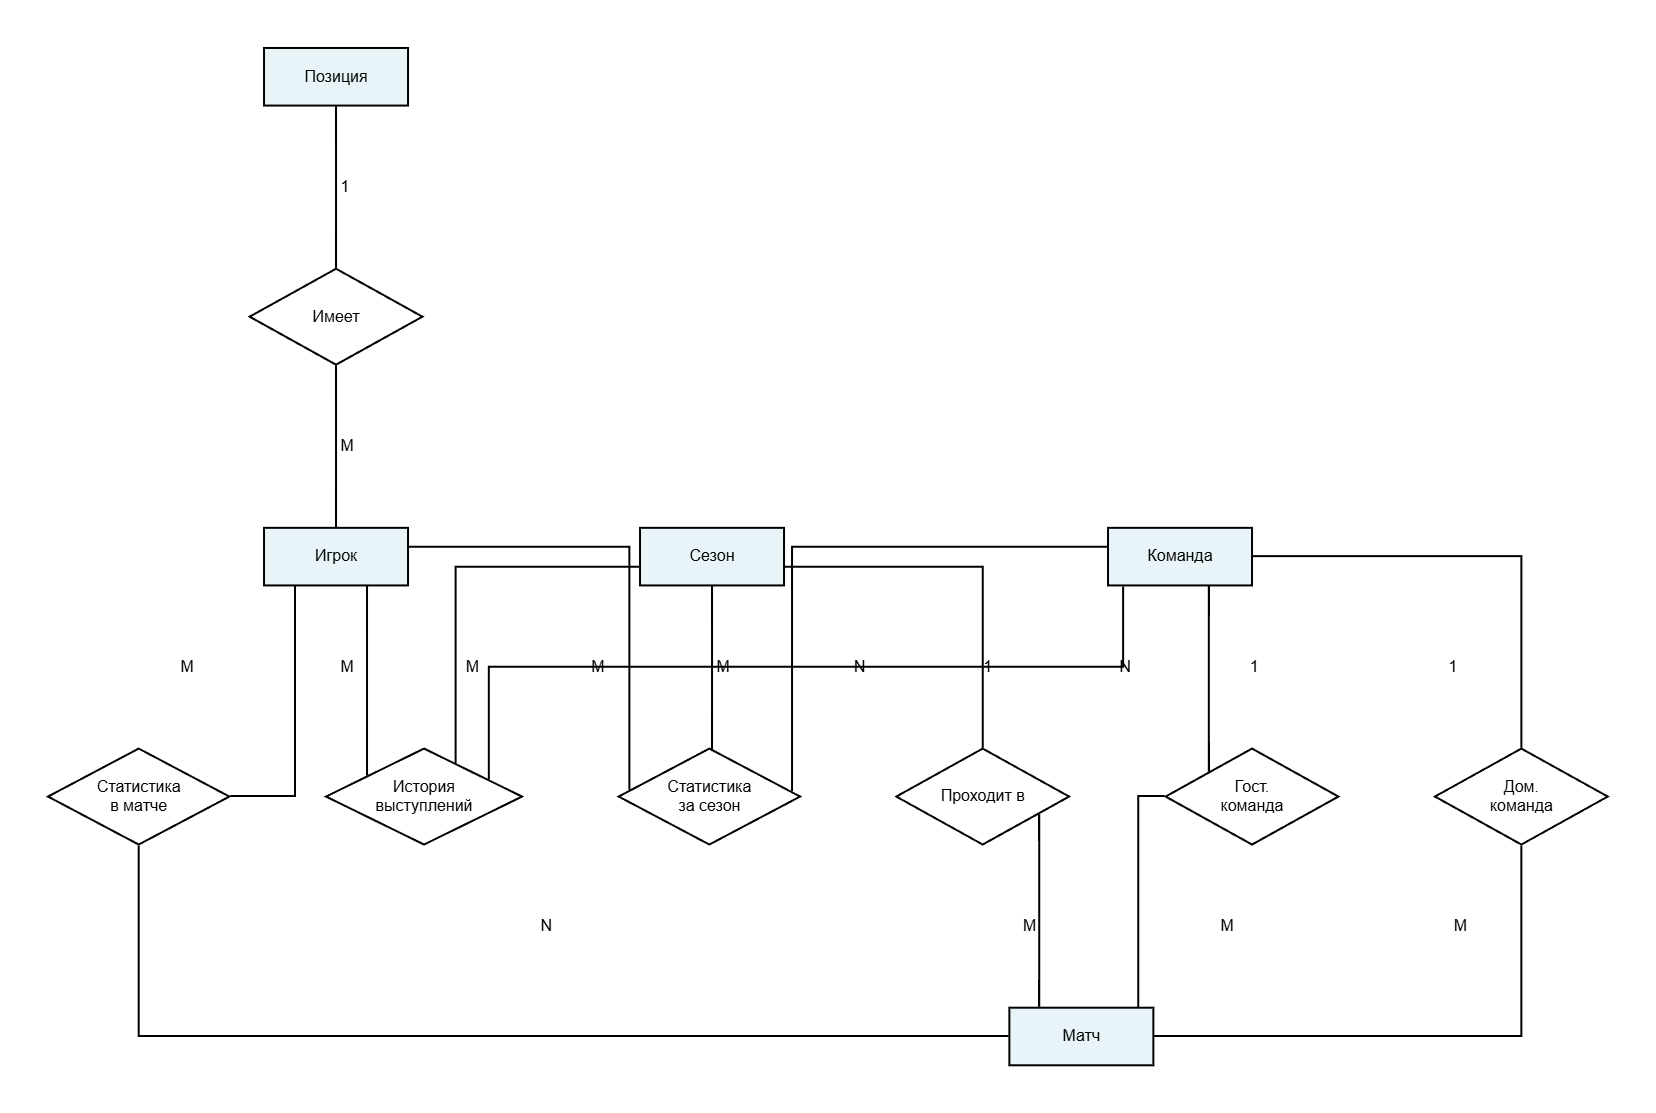
\includegraphics[width=\textwidth]{../img/333.png}
\caption{ER-диаграмма в нотации Чена}
\label{fig:er-chen}
\end{figure}

\subsection{Роли пользователей и варианты использования}\label{sec:use-cases}

Система предусматривает три роли пользователей.
\begin{enumerate}
    \item администратор~--- полное управление структурой и содержимым
          хранилища: создание и изменение схемы, загрузка и сопровождение
          данных, резервное копирование;
    \item аналитик~--- чтение данных и запуск расчётных процедур для
          получения производных показателей;
    \item читатель~--- доступ к агрегированным данным через
          представления; изменение содержимого базовых таблиц недоступно.
\end{enumerate}

Соответствие ролей и допустимых операций задаётся тремя вариантами использования.
\begin{enumerate}
    \item просмотр статистики~--- получение сведений о матчах, игроках
          и командах, агрегированных показателях и рейтингах; доступно всем
          ролям;
    \item расчёт метрик~--- вычисление продвинутых показателей
          (PER, BPM, eFG\%, TS\%, USG\%) на основе первичных данных; доступно
          аналитику и администратору;
    \item управление данными~--- загрузка данных о матчах, обновление
          справочников, изменение схемы; доступно только администратору.
\end{enumerate}

\begin{figure}[H]
\centering
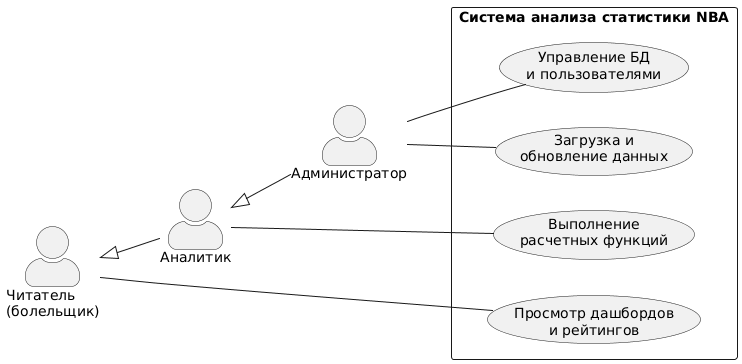
\includegraphics[width=\textwidth]{../img/22.png}
\caption{Диаграмма вариантов использования}
\label{fig:usecase}
\end{figure}

\section{Выбор модели данных}

Для выбора подходящей модели хранения данных проведём сравнение трёх основных
парадигм, опираясь на принципы проектирования дата-интенсивных приложений~\cite{kleppmann}.

\textbf{Документо-ориентированные СУБД (MongoDB, Couchbase)}. Как отмечают
П.~Садаладж и М.~Фаулер~\cite{fowler}, такие базы данных оптимальны для хранения агрегированных
JSON-документов без жёсткой схемы (schema-less). Сырая статистика матча (Box Score)
естественно ложится в документную модель. Однако данный подход существенно
проигрывает в производительности при многомерных агрегациях по нескольким сезонам и не
поддерживает декларативную валидацию бизнес-правил на уровне хранилища.

\textbf{Колоночные СУБД (ClickHouse и аналогичные OLAP-системы)} ориентированы
на аналитику больших объёмов данных: хранение по столбцам многократно ускоряет
агрегирующие запросы (GROUP BY, SUM, AVG)~\cite{clickhouse}. Однако, как указывается
в теории баз данных, OLAP-системы не обеспечивают полноценных транзакций ACID
при смешанных нагрузках, что критично для согласованности данных матчей, и
существенно усложняют реализацию JOIN-запросов между справочниками и таблицами фактов.

\textbf{Реляционные СУБД (PostgreSQL, MySQL)} гарантируют строгую согласованность
данных (ACID) и обладают мощным оптимизатором SQL-запросов~\cite{date}. В отличие
от NoSQL, реляционная модель (schema-on-write) позволяет встроить валидацию
бизнес-логики непосредственно в СУБД через ограничения (CHECK) и триггеры,
что обеспечивает достоверность спортивной статистики.

\begin{table}[H]
\centering
\footnotesize
\setlength{\tabcolsep}{3pt}
\renewcommand{\arraystretch}{1.2}
\caption{Сравнительная характеристика моделей хранения данных}
\label{tab:arch-compare}
\begin{tabularx}{\textwidth}{|>{\RaggedRight\arraybackslash}p{3.2cm}
  |>{\RaggedRight\arraybackslash}X
  |>{\RaggedRight\arraybackslash}X
  |>{\RaggedRight\arraybackslash}X|}
\hline
\textbf{Критерий} & \textbf{Документная СУБД} & \textbf{Колоночная СУБД}
  & \textbf{Реляционная СУБД} \\
\hline
Контроль над схемой & Гибкая (schema-less) & Жёсткая по столбцам
  & Строгая (schema-on-write) \\
\hline
Транзакционность (ACID) & Частичная & Не поддерживается при OLTP-нагрузке
  & Полная \\
\hline
Сложные JOIN-запросы & Затруднены & Затруднены & Встроенная поддержка \\
\hline
Агрегации по сезонам & Средняя (MapReduce) & Высокая (по столбцам)
  & Высокая (оптимизатор SQL) \\
\hline
Валидация бизнес-логики & На уровне приложения & На уровне приложения
  & Встроенная (триггеры, CHECK) \\
\hline
Соответствие структуре матча & Идеальное (JSON) & Требует денормализации
  & Требует декомпозиции \\
\hline
\end{tabularx}
\end{table}

Колоночные СУБД демонстрируют преимущество преимущественно при объёмах от десятков
миллионов строк и строго однородной аналитической нагрузке класса OLAP. Рассматриваемая
система предполагает смешанный профиль использования. Процедура обновления сезонной
статистики выполняет ресурсоёмкие транзакционные операции слияния для сотен записей
одновременно. Кроме того, необходимость ретроспективной корректировки данных из-за
ошибок в официальных протоколах матчей требует гарантированно атомарного обновления
сразу нескольких связанных таблиц.

При целевом объёме таблицы фактов порядка 200\,000 строк классическая реляционная
база данных способна обрабатывать агрегирующие запросы без существенных задержек.
Для наиболее востребованных аналитических выборок, таких как списки лидеров и сводные
турнирные таблицы, применяется кэширование в Redis~\cite{redis}, что полностью
нивелирует отставание в скорости чтения от специализированных аналитических решений.
Использование колоночной СУБД при таком масштабе неизбежно привело бы к усложнению
системы за счёт выделения отдельного транзакционного хранилища для операций записи.
Подобная архитектурная избыточность не даст измеримого выигрыша в производительности.

Таким образом, с учётом требований к транзакционной целостности и предсказуемого
объёма данных, оптимальным выбором является реляционная модель~\cite{date,connolly}.
В качестве основной СУБД выбран PostgreSQL~15~\cite{postgres}.

\section*{Вывод}

Сформулированы функциональные и нефункциональные требования и ограничения;
определён перечень метрик и правила их вычисления. Выделены восемь сущностей,
установлены связи «многие-ко-многим» через таблицы фактов, описаны три
пользовательские роли. По результатам сравнения моделей хранения данных выбрана
реляционная модель (PostgreSQL~15): она единственная обеспечивает полный ACID,
произвольные JOIN-запросы и встроенную валидацию бизнес-логики. Сравнительный
анализ существующих систем (NBA.com Stats, Basketball-Reference, ESPN Stats)
подтвердил отсутствие у них произвольных аналитических запросов, управляемого
ролевого доступа и воспроизводимого локального хранения данных, что
обусловливает целесообразность разработки специализированной базы данных.
Диаграмма вариантов использования и ER-диаграмма приведены на
рисунках~\ref{fig:usecase} и~\ref{fig:er-chen}.
	\chapter{Конструкторский раздел}

\section{Логическое проектирование базы данных}\label{sec:db-design}

Схема базы данных (рисунок~\ref{fig:relational-schema}) включает восемь
таблиц. Факты хранятся в \newline \texttt{game\_player\_stats}, денормализованная
витрина \texttt{player\_season\_stats} ускоряет аналитические выборки.
Справочники используют суррогатные ключи.

\begin{figure}[H]
\centering
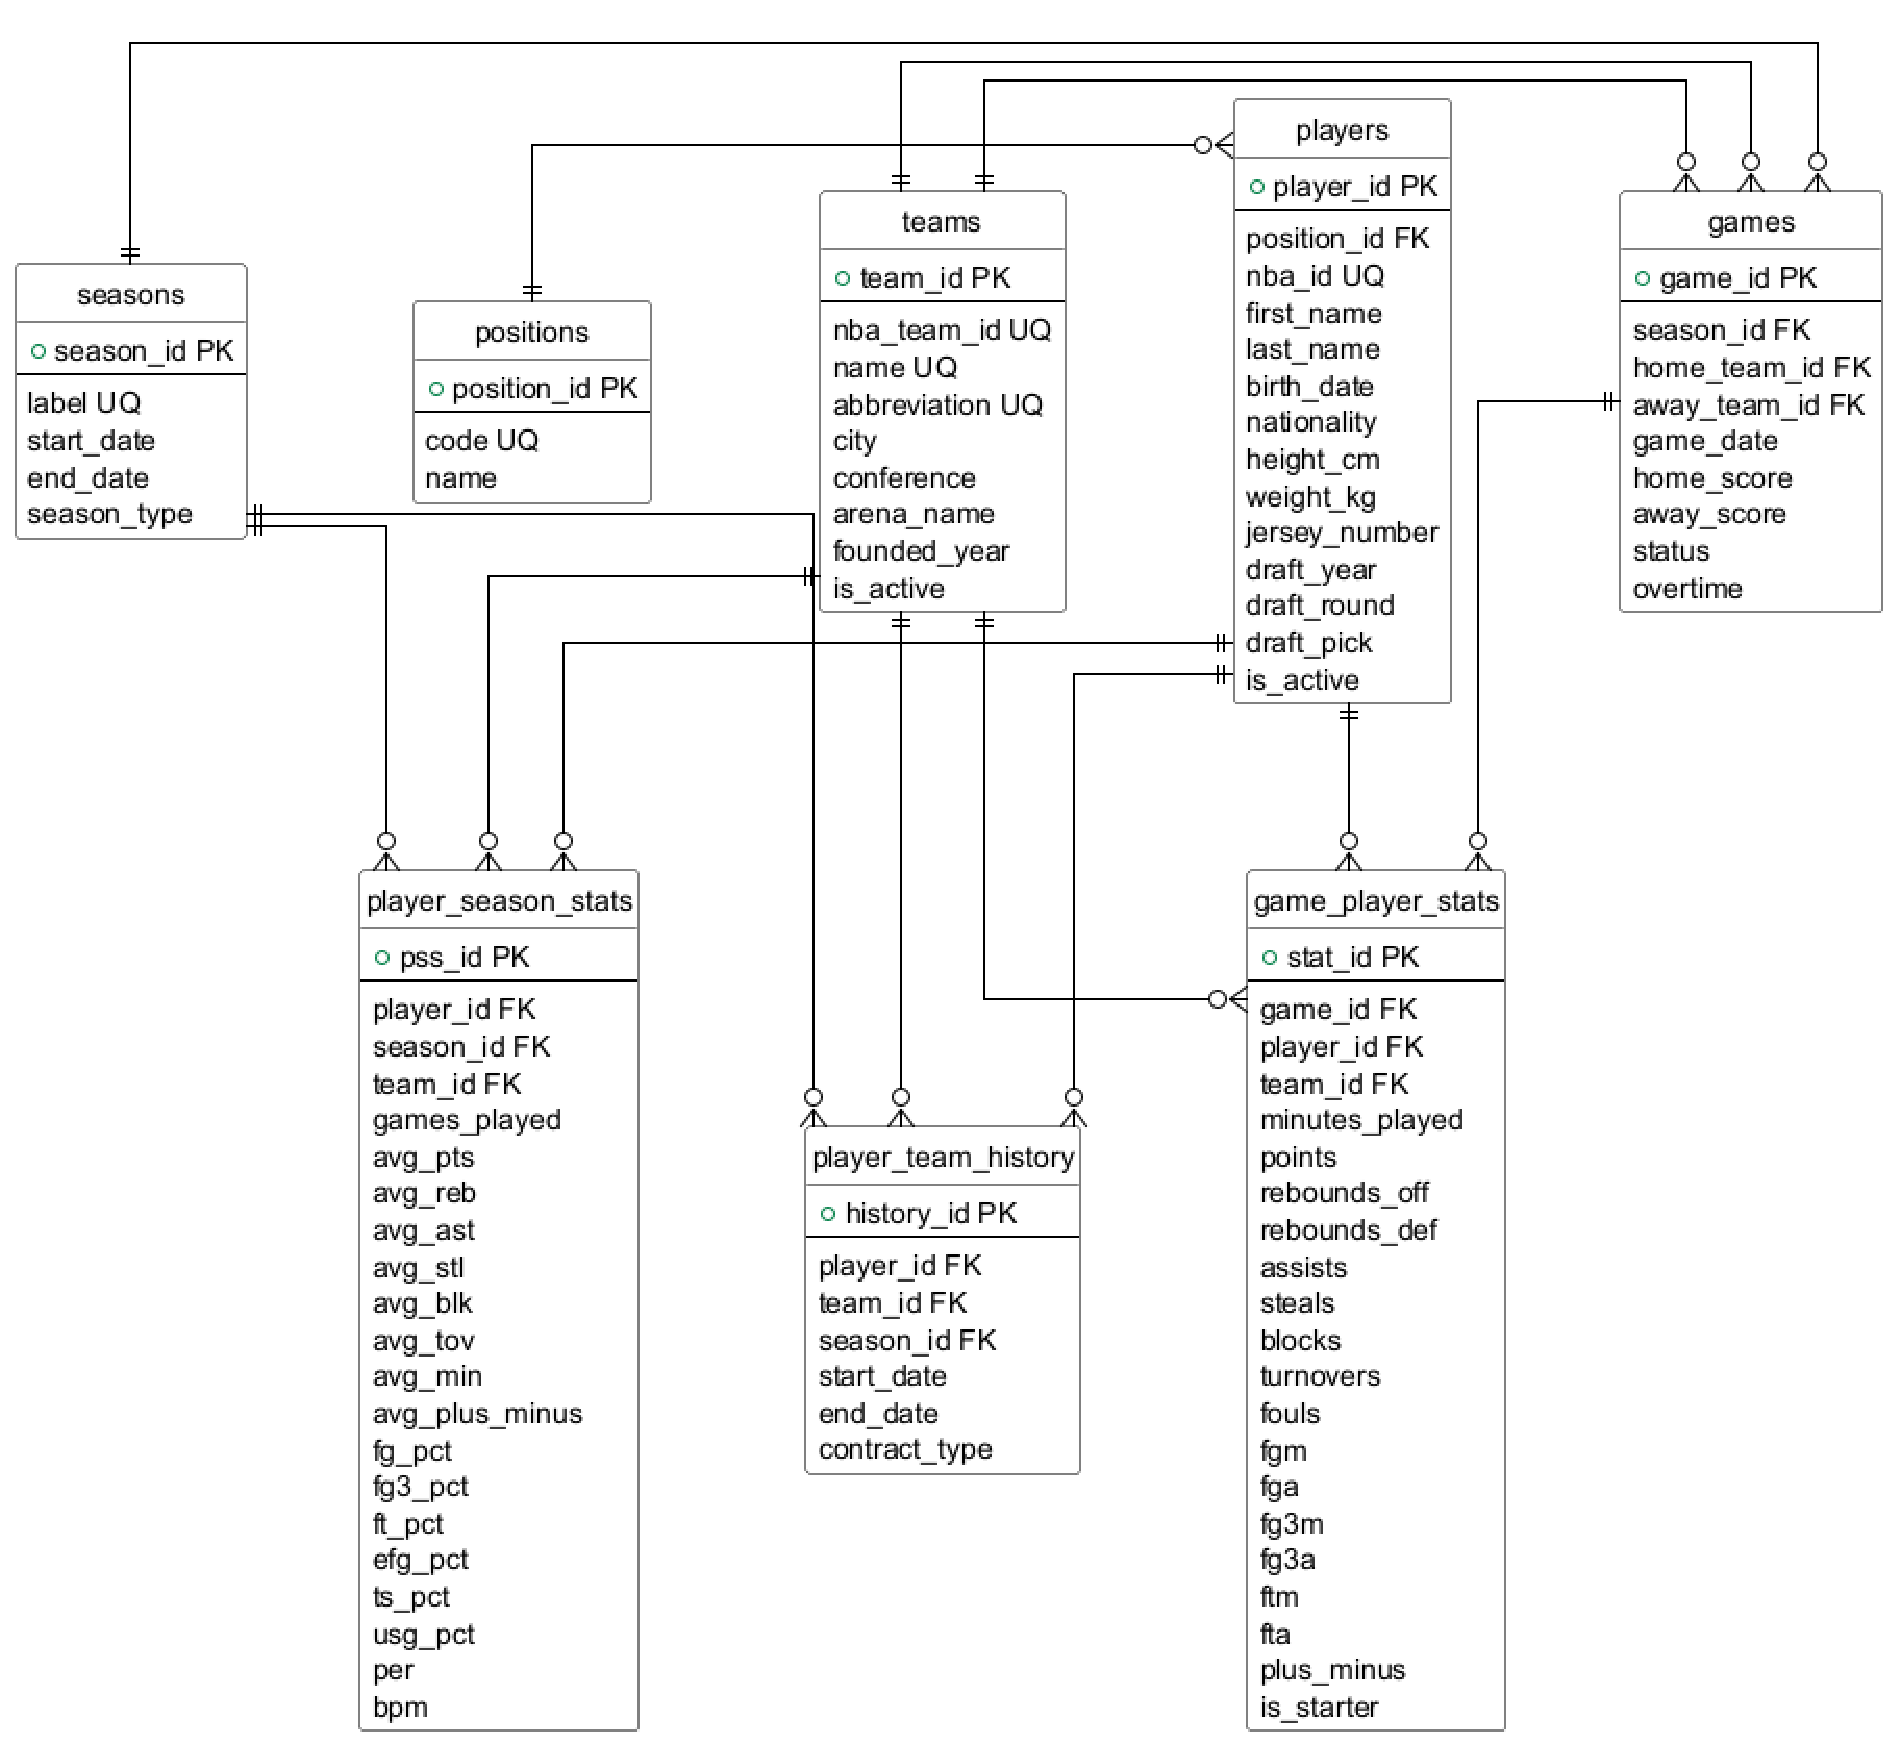
\includegraphics[width=1\textwidth]{../img/relational_schema.pdf}
\caption{Схема реляционной базы данных}
\label{fig:relational-schema}
\end{figure}

{\footnotesize\setlength{\tabcolsep}{4pt}\renewcommand{\arraystretch}{1.12}%

{\normalsize
Для нормализованного хранения игровых позиций спроектирована таблица
\texttt{positions} (табл.~\ref{tab:pos}).
}

\begin{table}[H]
\caption{Справочник игровых позиций}
\label{tab:pos}
\centering
\begin{tabular}{|p{0.22\textwidth}|p{0.28\textwidth}|p{0.42\textwidth}|}
\hline
\textbf{Атрибут} & \textbf{Тип} & \textbf{Ключ / назначение} \\
\hline
position\_id & Целочисленный (автоинкремент) & первичный ключ \\
\hline
code & Строковый фиксированной длины & уникальный; код позиции \\
\hline
name & Строковый & полное название позиции \\
\hline
\end{tabular}
\end{table}

{\normalsize
Интервалы проведения соревнований описываются таблицей
\texttt{seasons} (табл.~\ref{tab:seasons}).
}

\begin{table}[H]
\caption{Справочник сезонов}
\label{tab:seasons}
\centering
\begin{tabular}{|p{0.22\textwidth}|p{0.28\textwidth}|p{0.42\textwidth}|}
\hline
\textbf{Атрибут} & \textbf{Тип} & \textbf{Ключ / назначение} \\
\hline
season\_id & Целочисленный (автоинкремент) & первичный ключ \\
\hline
label & Строковый & уникальный; обозначение сезона, в частности формата 2025-26 \\
\hline
start\_date & Дата & дата начала сезона \\
\hline
end\_date & Дата & дата окончания сезона \\
\hline
season\_type & Строковый & Regular, Playoff, Preseason \\
\hline
\end{tabular}
\end{table}

{\normalsize
Информация о баскетбольных клубах и их домашних аренах хранится в таблице
\texttt{teams} (табл.~\ref{tab:teams}).
}

\begin{table}[H]
\caption{Справочник команд}
\label{tab:teams}
\centering
\begin{tabular}{|p{0.22\textwidth}|p{0.28\textwidth}|p{0.42\textwidth}|}
\hline
\textbf{Атрибут} & \textbf{Тип} & \textbf{Ключ / назначение} \\
\hline
team\_id & Целочисленный (автоинкремент) & первичный ключ \\
\hline
nba\_team\_id & Целочисленный & уникальный; id на NBA.com \\
\hline
name & Строковый & уникальный; полное название \\
\hline
abbreviation & Строковый фиксированной длины & уникальный; аббревиатура \\
\hline
city & Строковый & город базирования \\
\hline
conference & Строковый & допустимые значения: East, West \\
\hline
arena\_name & Строковый & домашняя арена \\
\hline
founded\_year & Целочисленный & год основания \\
\hline
is\_active & Логический & признак активной команды \\
\hline
\end{tabular}
\end{table}

{\normalsize
Для хранения персональных и антропометрических данных баскетболистов
разработана таблица \texttt{players} (табл.~\ref{tab:players}).
}

\begin{table}[H]
\caption{Справочник игроков}
\label{tab:players}
\centering
\begin{tabular}{|p{0.22\textwidth}|p{0.28\textwidth}|p{0.42\textwidth}|}
\hline
\textbf{Атрибут} & \textbf{Тип} & \textbf{Ключ / назначение} \\
\hline
player\_id & Целочисленный (автоинкремент) & первичный ключ \\
\hline
position\_id & Целочисленный & внешний ключ $\rightarrow$ \texttt{positions} \\
\hline
nba\_id & Целочисленный & уникальный; id на NBA.com \\
\hline
first\_name & Строковый & имя \\
\hline
last\_name & Строковый & фамилия \\
\hline
birth\_date & Дата & дата рождения \\
\hline
nationality & Строковый & гражданство \\
\hline
height\_cm & Целочисленный & рост (см) \\
\hline
weight\_kg & Целочисленный & вес (кг) \\
\hline
jersey\_number & Целочисленный & номер на майке (0--99) \\
\hline
draft\_year & Целочисленный & год драфта \\
\hline
draft\_round & Целочисленный & раунд драфта (1 или 2) \\
\hline
draft\_pick & Целочисленный & номер выбора на драфте \\
\hline
is\_active & Логический & действующий игрок \\
\hline
\end{tabular}
\end{table}

{\normalsize
Сведения о проведённых и запланированных матчах фиксируются в таблице
\texttt{games} (табл.~\ref{tab:games}).
}

\begin{table}[H]
\caption{Матчи}
\label{tab:games}
\centering
\begin{tabular}{|p{0.22\textwidth}|p{0.28\textwidth}|p{0.42\textwidth}|}
\hline
\textbf{Атрибут} & \textbf{Тип} & \textbf{Ключ / назначение} \\
\hline
game\_id & Целочисленный (автоинкремент) & первичный ключ \\
\hline
season\_id & Целочисленный & внешний ключ $\rightarrow$ \texttt{seasons} \\
\hline
home\_team\_id & Целочисленный & внешний ключ $\rightarrow$ \texttt{teams}; команда-хозяин \\
\hline
away\_team\_id & Целочисленный & внешний ключ $\rightarrow$ \texttt{teams}; команда-гость \\
\hline
game\_date & Дата & дата матча \\
\hline
home\_score & Целочисленный & счёт хозяев \\
\hline
away\_score & Целочисленный & счёт гостей \\
\hline
status & Строковый & Finished, Scheduled, Postponed \\
\hline
overtime & Целочисленный & число овертаймов (0--6) \\
\hline
\end{tabular}
\end{table}

{\normalsize
Атомарные факты результативности игроков в конкретном матче (основная таблица
фактов) сохраняются в детализированной таблице \texttt{game\_player\_stats}
(табл.~\ref{tab:gps}).
}

\begin{table}[H]
\caption{Факты статистики игрока в матче}
\label{tab:gps}
\centering
\begin{tabular}{|p{0.22\textwidth}|p{0.28\textwidth}|p{0.42\textwidth}|}
\hline
\textbf{Атрибут} & \textbf{Тип} & \textbf{Ключ / назначение} \\
\hline
stat\_id & Целочисленный (автоинкремент) & первичный ключ \\
\hline
game\_id & Целочисленный & внешний ключ $\rightarrow$ \texttt{games}; каскадное удаление \\
\hline
player\_id & Целочисленный & внешний ключ $\rightarrow$ \texttt{players}; запрет удаления при зависимых записях \\
\hline
team\_id & Целочисленный & внешний ключ $\rightarrow$ \texttt{teams}; запрет удаления при зависимых записях \\
\hline
minutes\_played & Вещественный & минуты на площадке \\
\hline
points & Целочисленный & очки (только неотрицательные значения) \\
\hline
rebounds\_off & Целочисленный & подборы в нападении \\
\hline
rebounds\_def & Целочисленный & подборы в защите \\
\hline
assists & Целочисленный & передачи \\
\hline
steals & Целочисленный & перехваты \\
\hline
blocks & Целочисленный & блоки \\
\hline
turnovers & Целочисленный & потери \\
\hline
fouls & Целочисленный & фолы (диапазон 0--6) \\
\hline
fgm, fga & Целочисленный & попадания и попытки с игры \\
\hline
fg3m, fg3a & Целочисленный & попадания и попытки с трёхочковой \\
\hline
ftm, fta & Целочисленный & попадания и попытки штрафных \\
\hline
plus\_minus & Целочисленный & показатель плюс-минус \\
\hline
is\_starter & Логический & признак стартового состава \\
\hline
\multicolumn{3}{|p{\dimexpr\textwidth-2\tabcolsep-2\arrayrulewidth\relax}|}{%
\textbf{Ограничение уникальности:} \texttt{(game\_id, player\_id)}~---
единственность записи игрока в матче} \\
\hline
\end{tabular}
\end{table}

} % end footnotesize (таблицы)

В таблице \texttt{game\_player\_stats} пара полей \texttt{game\_id} и
\texttt{player\_id} закреплена ограничением уникальности. Это исключает
дублирование строк статистики одного игрока в одном матче.

{\footnotesize\setlength{\tabcolsep}{4pt}\renewcommand{\arraystretch}{1.12}%

{\normalsize
Агрегированные статистические показатели и расчётные метрики эффективности за
сезон материализуются в таблице \texttt{player\_season\_stats}
(табл.~\ref{tab:pss}).
}

\begin{table}[H]
\caption{Агрегаты статистики за сезон}
\label{tab:pss}
\centering
\begin{tabular}{|p{0.22\textwidth}|p{0.28\textwidth}|p{0.42\textwidth}|}
\hline
\textbf{Атрибут} & \textbf{Тип} & \textbf{Ключ / назначение} \\
\hline
pss\_id & Целочисленный (автоинкремент) & первичный ключ \\
\hline
player\_id & Целочисленный & внешний ключ $\rightarrow$ \texttt{players}; часть ограничения уникальности \\
\hline
season\_id & Целочисленный & внешний ключ $\rightarrow$ \texttt{seasons}; часть ограничения уникальности \\
\hline
team\_id & Целочисленный & внешний ключ $\rightarrow$ \texttt{teams}; часть ограничения уникальности \\
\hline
games\_played & Целочисленный & число игр в сезоне \\
\hline
avg\_pts & Вещественный & средние очки за матч \\
\hline
avg\_reb & Вещественный & средние подборы за матч \\
\hline
avg\_ast & Вещественный & средние передачи за матч \\
\hline
avg\_stl & Вещественный & средние перехваты за матч \\
\hline
avg\_blk & Вещественный & средние блоки за матч \\
\hline
avg\_tov & Вещественный & средние потери за матч \\
\hline
avg\_min & Вещественный & среднее время на площадке \\
\hline
avg\_plus\_minus & Вещественный & средний плюс-минус \\
\hline
fg\_pct & Вещественный & процент попаданий с игры ($\in [0,1]$) \\
\hline
fg3\_pct & Вещественный & процент трёхочковых ($\in [0,1]$) \\
\hline
ft\_pct & Вещественный & процент штрафных ($\in [0,1]$) \\
\hline
efg\_pct & Вещественный & eFG\% (доля 0--1) \\
\hline
ts\_pct & Вещественный & TS\% (доля 0--1) \\
\hline
usg\_pct & Вещественный & USG\% (доля 0--1) \\
\hline
per & Вещественный & PER \\
\hline
bpm & Вещественный & BPM \\
\hline
\multicolumn{3}{|p{\dimexpr\textwidth-2\tabcolsep-2\arrayrulewidth\relax}|}{%
\textbf{Ограничение уникальности:} \texttt{(player\_id, season\_id, team\_id)}~---
не более одной строки агрегата на игрока, сезон и команду} \\
\hline
\end{tabular}
\end{table}

{\normalsize
Трансферы игроков фиксируются в таблице
\texttt{player\_team\_history} (табл.~\ref{tab:pth}).
}

\begin{table}[H]
\caption{История выступлений игроков}
\label{tab:pth}
\centering
\begin{tabular}{|p{0.22\textwidth}|p{0.28\textwidth}|p{0.42\textwidth}|}
\hline
\textbf{Атрибут} & \textbf{Тип} & \textbf{Ключ / назначение} \\
\hline
history\_id & Целочисленный (автоинкремент) & первичный ключ \\
\hline
player\_id & Целочисленный & внешний ключ $\rightarrow$ \texttt{players}; часть ограничения уникальности \\
\hline
team\_id & Целочисленный & внешний ключ $\rightarrow$ \texttt{teams} \\
\hline
season\_id & Целочисленный & внешний ключ $\rightarrow$ \texttt{seasons} \\
\hline
start\_date & Дата & дата начала выступления \\
\hline
end\_date & Дата & дата окончания (не задана~--- по сей день) \\
\hline
contract\_type & Строковый & Standard, Two-Way, 10-Day и др. \\
\hline
\end{tabular}
\end{table}
} % end footnotesize

\subsection{Соответствие нормальным формам}

Проектирование транзакционной части схемы выполнено с соблюдением требований нормализации до третьей нормальной формы включительно. Это минимизирует избыточность данных и предотвращает аномалии модификации. Для аналитической витрины \newline \texttt{player\_season\_stats} применена контролируемая денормализация с целью оптимизации скорости выполнения запросов~\cite{date}.

\textbf{Первая нормальная форма.} В соответствии с требованиями первой нормальной формы все атрибуты отношений являются атомарными, а скрытые массивы и списки отсутствуют. В схеме нет составных или многозначных атрибутов. Полное имя игрока декомпозировано на скалярные атрибуты имени и фамилии. Рост и вес хранятся как отдельные числовые значения. История трансферов вынесена в отдельную таблицу. Базовые таблицы схемы соответствуют требованиям первой нормальной формы.

\textbf{Вторая нормальная форма.} Отношение находится во второй нормальной форме, если оно соответствует первой нормальной форме и каждый неключевой атрибут функционально полно зависит от любого потенциального ключа. Неключевым является атрибут, не входящий в состав ни одного потенциального ключа.

Потенциальные ключи и неключевые атрибуты спроектированных таблиц приведены в таблице~\ref{tab:potential_keys}.

{\footnotesize\setlength{\tabcolsep}{4pt}\renewcommand{\arraystretch}{1.15}
\begin{table}[H]
\caption{Потенциальные ключи и неключевые атрибуты спроектированных таблиц}
\label{tab:potential_keys}
\centering
\begin{tabular}{|>{\RaggedRight\arraybackslash}p{0.28\textwidth}|>{\RaggedRight\arraybackslash}p{0.26\textwidth}|>{\RaggedRight\arraybackslash}p{0.34\textwidth}|}
\hline
\textbf{Таблица} & \textbf{Потенциальные ключи} & \textbf{Неключевые атрибуты} \\
\hline
\texttt{positions} & \{\texttt{position\_id}\}, \{\texttt{code}\} & \texttt{name} \\
\hline
\texttt{seasons} & \{\texttt{season\_id}\}, \{\texttt{label}\} & \texttt{start\_date}, \texttt{end\_date}, \texttt{season\_type} \\
\hline
\texttt{teams} & \{\texttt{team\_id}\}, \{\texttt{nba\_team\_id}\}, \{\texttt{name}\}, \{\texttt{abbreviation}\} & \texttt{city}, \texttt{conference}, \texttt{arena\_name}, \texttt{founded\_year}, \texttt{is\_active} \\
\hline
\texttt{players} & \{\texttt{player\_id}\}, \{\texttt{nba\_id}\} & \texttt{first\_name}, \texttt{last\_name}, \texttt{birth\_date}, \texttt{nationality}, \texttt{height\_cm}, \texttt{weight\_kg}, \texttt{position\_id}, \texttt{jersey\_number}, \texttt{is\_active}, \texttt{draft\_year}, \texttt{draft\_round}, \texttt{draft\_pick} \\
\hline
\texttt{games} & \{\texttt{game\_id}\} & \texttt{season\_id}, \texttt{home\_team\_id}, \texttt{away\_team\_id}, \texttt{game\_date}, \texttt{home\_score}, \texttt{away\_score}, \texttt{status}, \texttt{overtime} \\
\hline
\texttt{player\_team\_history} & \{\texttt{history\_id}\}, \{\texttt{player\_id}, \texttt{season\_id}, \texttt{team\_id}\} & \texttt{start\_date}, \texttt{end\_date}, \texttt{contract\_type} \\
\hline
\texttt{game\_player\_stats} & \{\texttt{stat\_id}\}, \{\texttt{game\_id}, \texttt{player\_id}\} & \texttt{team\_id}, \texttt{minutes\_played}, \texttt{points}, \texttt{rebounds\_off}, \texttt{rebounds\_def}, \texttt{assists}, \texttt{steals}, \texttt{blocks}, \texttt{turnovers}, \texttt{fouls}, \texttt{fgm}, \texttt{fga}, \texttt{fg3m}, \texttt{fg3a}, \texttt{ftm}, \texttt{fta}, \texttt{plus\_minus}, \texttt{is\_starter} \\
\hline
\end{tabular}
\end{table}}

Для таблиц \texttt{positions}, \texttt{seasons}, \texttt{teams}, \texttt{players} и \texttt{games} все потенциальные ключи состоят из одного атрибута, поэтому частичная зависимость в них невозможна.

Таблицы \texttt{game\_player\_stats} и \texttt{player\_team\_history} имеют составные потенциальные ключи. В \texttt{game\_player\_stats} ключ включает идентификаторы матча и игрока; неключевые атрибуты характеризуют результат конкретного игрока в конкретном матче, и ни один показатель не определяется только идентификатором игрока или только идентификатором матча. Атрибут команды также зависит от обеих частей ключа из-за возможности переходов игрока в течение сезона. В \texttt{player\_team\_history} составной ключ образуют идентификаторы игрока, сезона и команды: одна запись описывает отдельный период выступления, а атрибуты дат начала и окончания и типа контракта зависят от полного ключа, а не от его части. Таким образом, частичные зависимости устранены, и схема соответствует требованиям второй нормальной формы.

\textbf{Третья нормальная форма.} Отношение находится в третьей нормальной форме, если оно соответствует второй нормальной форме и не содержит транзитивных функциональных зависимостей неключевых атрибутов от потенциальных ключей. Это означает отсутствие функциональных зависимостей между самими неключевыми атрибутами.

Анализ неключевых атрибутов базовых таблиц:
\begin{enumerate}
    \item \texttt{positions}: содержит единственный неключевой атрибут названия позиции, что исключает взаимосвязи неключевых атрибутов;
    \item \texttt{seasons}: неключевые атрибуты дат начала и окончания, а также типа сезона не связаны транзитивными зависимостями друг с другом;
    \item \texttt{teams}: неключевые атрибуты города, конференции, названия арены, года основания и активности описывают свойства тридцати уникальных клубов ассоциации и не образуют транзитивных функциональных зависимостей;
    \item \texttt{players}: неключевые атрибуты имени, фамилии, даты рождения, гражданства, физических параметров и драфта не связаны транзитивными зависимостями. Текстовое название позиции вынесено во внешнюю таблицу \texttt{positions}, что исключает транзитивную зависимость через внешний ключ;
    \item \texttt{games}: неключевые атрибуты дат, счета и статуса не связаны транзитивными зависимостями. Названия команд и городов вынесены в таблицу \texttt{teams}, что устраняет транзитивные зависимости через внешние ключи команд;
    \item \texttt{game\_player\_stats}: неключевые атрибуты представляют собой индивидуальные статистические показатели игрока в матче, не связанные транзитивными зависимостями;
    \item \texttt{player\_team\_history}: неключевые атрибуты дат выступления и типа контракта не имеют функциональных зависимостей между собой.
\end{enumerate}

Базовые таблицы схемы соответствуют требованиям третьей нормальной формы.

Аналитическая витрина \texttt{player\_season\_stats} спроектирована как денормализованное отношение. Её потенциальными ключами являются \{\texttt{pss\_id}\} и \{\texttt{player\_id}, \texttt{season\_id}, \texttt{team\_id}\}. Как самостоятельное отношение она удовлетворяет требованиям третьей нормальной формы, поскольку её неключевые атрибуты, представляющие собой средние значения и интегральные метрики, функционально независимы друг от друга. Хранение производных данных в данном случае является контролируемой денормализацией. Данное решение принято с целью повышения производительности аналитических запросов за счет предварительного расчета агрегатов. Это исключает необходимость выполнения ресурсоемких группировок по таблице фактов \texttt{game\_player\_stats} на этапе чтения.
\subsection{Проектирование представлений}

Инкапсуляция базовых таблиц и ограничение прямого доступа спроектированы
через три представления:
\begin{enumerate}
    \item \texttt{v\_player\_rankings}~--- инкапсулирует операцию объединения между
          таблицей агрегатов \texttt{player\_season\_stats} и справочниками
          \texttt{players}, \texttt{teams}. Предоставляет денормализованный
          сводный рейтинг игроков за сезон по базовым и расчётным метрикам,
          скрывая от клиента сложность объединения таблиц;
    \item \texttt{v\_team\_stats}~--- спроектирован для обеспечения функционального требования
          динамического расчёта командной статистики. Выполняет агрегацию
          данных таблицы \newline \texttt{game\_player\_stats} с применением
          статистических функций среднего и суммы в разрезе команды
          и сезона, исключая необходимость хранения избыточной таблицы
          командных фактов;
    \item \texttt{v\_top\_players}~--- обеспечивает безопасность данных для
          публичной роли \texttt{reader}. Является фильтрованным подмножеством
          представления \texttt{v\_player\_rankings} с ограничением выборки
          и сортировкой лидеров по метрике PER.
\end{enumerate}

\subsection{Проектирование индексов}\label{subsec:indexes}

Для обеспечения производительности аналитических запросов (согласно п.~\ref{sec:nfr})
спроектировано создание следующих индексов на базе структуры B-tree~\cite{connolly}:
\begin{enumerate}
    \item \texttt{idx\_gps\_player\_id}~--- индекс по полю \texttt{player\_id}
          в таблице \texttt{game\_player\_stats}; ускоряет выборку всех выступлений
          игрока для агрегации сезонной статистики;
    \item \texttt{idx\_gps\_team\_game}~--- составной индекс по полям
          \texttt{team\_id}, \texttt{game\_id} в таблице \texttt{game\_player\_stats};
          поддерживает агрегацию командной статистики в представлении
          \texttt{v\_team\_stats};
    \item \texttt{idx\_games\_season\_id}~--- индекс по полю \texttt{season\_id}
          в таблице \texttt{games}; ускоряет фильтрацию матчей по сезону;
    \item \texttt{idx\_games\_date}~--- индекс по полю \texttt{game\_date} в таблице
          \texttt{games}; обеспечивает диапазонную фильтрацию по дате проведения
          матча;
    \item \texttt{idx\_pss\_season}~--- индекс по полю \texttt{season\_id} в таблице
          \texttt{player\_season\_stats}; ускоряет выборку рейтингов за конкретный
          сезон;
    \item \texttt{idx\_players\_name}~--- составной индекс по полям
          \texttt{last\_name}, \texttt{first\_name} в таблице \texttt{players};
          поддерживает поиск игрока по фамилии.
\end{enumerate}

Для обеспечения уникальности записей в таблице \texttt{game\_player\_stats}
предусмотрен составной индекс по полям \texttt{(game\_id, player\_id)}, который
дополнительно покрывает запросы поиска по паре «матч~-- игрок». В качестве
алгоритмической основы для всех проектируемых индексов выбрана структура
сбалансированного дерева (B-tree), поскольку она обеспечивает логарифмическую
сложность поиска по предикатам равенства и диапазона.

% Общие параметры блок-схем (ГОСТ 19.701): единая ширина блоков
\newcommand{\flowchartBlockWidth}{6.8cm}
\newcommand{\flowchartBlockHeight}{0.85cm}
\newcommand{\flowchartRightShift}{6.3cm}      % отступ правой колонки (рис. 2.2--2.8)
\newcommand{\flowchartRightShiftSmall}{5.0cm} % компактная схема calculate_ts
\newcommand{\flowchartUpdateVGap}{1.28cm}     % верт. зазор для рис. 2.10
\newcommand{\flowchartUpdateMidExtra}{-0.4cm}   % pro3→pro4, pro4→pro5 (рис. 2.10)
\newcommand{\flowchartTinyVExtra}{-0.15cm}    % микро-добавка (рис. 2.3)
\newcommand{\flowchartDecExpExtra}{-0.45cm}   % dec1 → expected (рис. 2.2)

\tikzset{
  fc base/.style={font=\footnotesize, inner sep=4pt},
  fc arrow/.style={thick,->,>=stealth},
  fc startstop/.style={draw, rectangle, rounded corners=10pt,
    text width=\flowchartBlockWidth, minimum height=\flowchartBlockHeight,
    align=center, fill=white},
  fc process/.style={draw, rectangle,
    text width=\flowchartBlockWidth, minimum height=\flowchartBlockHeight,
    align=center, fill=white},
  fc predefined/.style={draw, rectangle,
    text width=\flowchartBlockWidth, minimum height=\flowchartBlockHeight,
    align=center, fill=white,
    path picture={
      \draw ([xshift=4pt]path picture bounding box.north west) --
            ([xshift=4pt]path picture bounding box.south west);
      \draw ([xshift=-4pt]path picture bounding box.north east) --
            ([xshift=-4pt]path picture bounding box.south east);
    }},
  fc io/.style={draw, trapezium, trapezium left angle=75, trapezium right angle=105,
    trapezium stretches=true,
    text width=\flowchartBlockWidth, minimum height=\flowchartBlockHeight,
    align=center, fill=white},
  fc decision/.style={draw, diamond, aspect=3.2,
    text width=5.0cm, inner sep=1pt,
    minimum height=\flowchartBlockHeight, align=center, fill=white},
}

\newcommand{\flowchartCalculateTs}{%
\begin{figure}[H]
\centering
\begin{tikzpicture}[
    fc base,
    node distance=1.5cm,
    startstop/.style={fc startstop},
    process/.style={fc process},
    io/.style={fc io},
    decision/.style={fc decision},
    arrow/.style={fc arrow}
]
\node (start)  [startstop] {Начало};
\node (pro1)   [process,  below of=start] {$PTS, FGA, FTA := \mathrm{SUM}(\ldots)$};
\node (pro2)   [process,  below of=pro1]
  {$D = 2 \cdot (\mathrm{FGA} + 0{,}44 \cdot \mathrm{FTA})$};
\node (dec1)   [decision, below of=pro2, yshift=-0.5cm] {$D = 0$?};
\node (pro3a)  [io,  right of=dec1, xshift=\flowchartRightShiftSmall] {Вывод:\\ значение не определено};
\node (pro3b)  [io,  below of=dec1, yshift=-0.5cm]
  {Возврат $\mathrm{PTS} / D$};
\node (stop)   [startstop, below of=pro3b] {Конец};

\draw [arrow] (start)  -- (pro1);
\draw [arrow] (pro1)   -- (pro2);
\draw [arrow] (pro2)   -- (dec1);
\draw [arrow] (dec1)   -- node[anchor=south] {Да}  (pro3a);
\draw [arrow] (dec1)   -- node[anchor=east]  {Нет} (pro3b);
\draw [arrow] (pro3b)  -- (stop);
\draw [arrow] (pro3a)  |- (stop);
\end{tikzpicture}
\caption{Схема алгоритма вычисления функции \texttt{calculate\_ts}}
\label{fig:algo-ts}
\end{figure}
}

\newcommand{\flowchartCalculateEfg}{%
\begin{figure}[H]
\centering
\begin{tikzpicture}[
    fc base,
    node distance=1.8cm,
    startstop/.style={fc startstop},
    process/.style={fc process},
    io/.style={fc io},
    decision/.style={fc decision},
    arrow/.style={fc arrow}
]
\node (start)  [startstop] {Начало};
\node (agg)    [process,  below of=start]
  {$FGM, FG3M, FGA := \mathrm{SUM}(\ldots)$ \\ из \texttt{game\_player\_stats}};
\node (dec1)   [decision, below of=agg] {$\mathrm{FGA} = 0$?};
\node (null1)  [io,  right of=dec1, xshift=\flowchartRightShift] {Вывод:\\ значение не определено};
\node (ret)    [io,  below of=dec1]
  {Возврат $\displaystyle\frac{\mathrm{FGM}+0{,}5\cdot\mathrm{FG3M}}{\mathrm{FGA}}$};
\node (stop)   [startstop, below of=ret] {Конец};

\draw [arrow] (start) -- (agg);
\draw [arrow] (agg)   -- (dec1);
\draw [arrow] (dec1)  -- node[above] {Да} (null1);
\draw [arrow] (dec1)  -- node[right] {Нет} (ret);
\draw [arrow] (ret)   -- (stop);
\draw [arrow] (null1.east) -- ++(0.6,0) |- (stop);
\end{tikzpicture}
\caption{Схема алгоритма вычисления функции \texttt{calculate\_efg}}
\label{fig:algo-efg}
\end{figure}
}

\newcommand{\flowchartCalculateUsg}{%
\begin{figure}[H]
\centering
\begin{tikzpicture}[
    fc base,
    node distance=1.8cm,
    startstop/.style={fc startstop},
    process/.style={fc process},
    io/.style={fc io},
    decision/.style={fc decision},
    arrow/.style={fc arrow}
]
\node (start)  [startstop] {Начало};
\node (tid)    [process,  below of=start]
  {Определить team\_id \\ (параметр или последняя игра)};
\node (dec0)   [decision, below of=tid, yshift=-0.2cm] {team\_id IS NULL?};
\node (null0)  [io,  right of=dec0, xshift=\flowchartRightShift] {Вывод:\\ значение не определено};
\node (aggP)   [process,  below of=dec0, yshift=-0.2cm]
  {$pFGA, pFTA, pTOV, pMP :=$ \\ $\mathrm{SUM}(\ldots)$ игрока};
\node (dec1)   [decision, below of=aggP, yshift=-0.2cm] {$pMP < 1$?};
\node (null1)  [io,  right of=dec1, xshift=\flowchartRightShift] {Вывод:\\ значение не определено};
\node (aggT)   [process,  below of=dec1, yshift=-0.2cm]
  {$tmFGA, tmFTA, tmTOV, tmMP :=$ \\ $\mathrm{SUM}(\ldots)$ команды};
\node (denom)  [process,  below of=aggT, yshift=-0.2cm]
  {$denom := pMP \cdot (tmFGA + 0{,}44 \cdot tmFTA + tmTOV)$};
\node (dec2)   [decision, below of=denom, yshift=-0.2cm] {denom $= 0$?};
\node (null2)  [io,  right of=dec2, xshift=\flowchartRightShift] {Вывод:\\ значение не определено};
\node (ret)    [io,  below of=dec2, yshift=-0.2cm]
  {Возврат $\displaystyle\frac{(pFGA+0{,}44\cdot pFTA+pTOV)\cdot\frac{tmMP}{5}}{denom}$};
\node (stop)   [startstop, below of=ret] {Конец};

\draw [arrow] (start) -- (tid);
\draw [arrow] (tid)   -- (dec0);
\draw [arrow] (dec0)  -- node[above] {Да} (null0);
\draw [arrow] (dec0)  -- node[right] {Нет} (aggP);
\draw [arrow] (aggP)  -- (dec1);
\draw [arrow] (dec1)  -- node[above] {Да} (null1);
\draw [arrow] (dec1)  -- node[right] {Нет} (aggT);
\draw [arrow] (aggT)  -- (denom);
\draw [arrow] (denom) -- (dec2);
\draw [arrow] (dec2)  -- node[above] {Да} (null2);
\draw [arrow] (dec2)  -- node[right] {Нет} (ret);
\draw [arrow] (ret)   -- (stop);

\draw [arrow] (null0.east) -- ++(0.5,0) coordinate (bus) |- (stop);
\draw [arrow] (null1.east) -- (null1.east -| bus);
\draw [arrow] (null2.east) -- (null2.east -| bus);
\end{tikzpicture}
\caption{Схема алгоритма вычисления функции \texttt{calculate\_usg}}
\label{fig:algo-usg}
\end{figure}
}

\newcommand{\flowchartCalculatePer}{%
\begin{figure}[H]
\centering
\begin{tikzpicture}[
    fc base,
    node distance=1.8cm,
    startstop/.style={fc startstop},
    process/.style={fc process},
    predefined/.style={fc predefined},
    io/.style={fc io},
    decision/.style={fc decision},
    arrow/.style={fc arrow}
]
\node (start) [startstop] {Начало};
\node (agg)   [process,  below of=start]
  {$PTS, TRB, AST, STL, BLK,$ \\ $TOV, PF, FGM/FGA, FTM/FTA, MP := \mathrm{SUM}(\ldots)$};
\node (dec1)  [decision, below of=agg] {$\mathrm{MP} < 50$?};
\node (null1) [io,  right of=dec1, xshift=\flowchartRightShift] {Вывод:\\ значение не определено};
\node (uper)  [process,  below of=dec1]
  {$\mathrm{uPER} = (\mathrm{PTS}+\mathrm{TRB}+\ldots - \mathrm{TOV}-\mathrm{PF}-\Delta\mathrm{FG}-0{,}44\cdot\Delta\mathrm{FT}) \cdot \tfrac{48}{\mathrm{MP}}$};
\node (lg)    [predefined,  below of=uper]
  {Вычисление lg\_aPER: \\ AVG(uPER) по игрокам с MP $> 100$};
\node (dec2)  [decision, below of=lg] {lg\_aPER $= 0$ или NULL?};
\node (fix)   [process,  right of=dec2, xshift=\flowchartRightShift] {lg\_aPER $= 15{,}0$};
\node (ret)   [io,  below of=dec2]
  {Возврат $\mathrm{uPER} \cdot 15\,/\,\mathrm{lg\_aPER}$};
\node (stop)  [startstop, below of=ret] {Конец};

\draw [arrow] (start) -- (agg);
\draw [arrow] (agg)   -- (dec1);
\draw [arrow] (dec1)  -- node[above] {Да} (null1);
\draw [arrow] (dec1)  -- node[right] {Нет} (uper);
\draw [arrow] (uper)  -- (lg);
\draw [arrow] (lg)    -- (dec2);
\draw [arrow] (dec2)  -- node[above] {Да} (fix);
\draw [arrow] (dec2)  -- node[right] {Нет} (ret);
\draw [arrow] (fix)   |- (ret);
\draw [arrow] (ret)   -- (stop);
\draw [arrow] (null1.east) -- ++(1.0,0) |- (stop);
\end{tikzpicture}
\caption{Схема алгоритма вычисления функции \texttt{calculate\_per}}
\label{fig:algo-per}
\end{figure}
}

\newcommand{\flowchartCalculateBpm}{%
\begin{figure}[H]
\centering
\begin{tikzpicture}[
    fc base,
    node distance=1.8cm,
    startstop/.style={fc startstop},
    process/.style={fc process},
    predefined/.style={fc predefined},
    io/.style={fc io},
    decision/.style={fc decision},
    arrow/.style={fc arrow}
]
\node (start) [startstop] {Начало};
\node (agg)   [process,  below of=start]
  {$PTS, TRB, AST, STL,$ \\ $BLK, TOV, PF, MP := \mathrm{SUM}(\ldots)$};
\node (dec1)  [decision, below of=agg] {$\mathrm{MP} < 50$?};
\node (null1) [io,  right of=dec1, xshift=\flowchartRightShift] {Вывод:\\ значение не определено};
\node (norm)  [process,  below of=dec1]
  {Нормировка на 100 мин: $X_{100} = X \cdot 100\,/\,\mathrm{MP}$};
\node (raw)   [process,  below of=norm]
  {raw $= 0{,}123\cdot\mathrm{PTS}_{100}+0{,}234\cdot\mathrm{TRB}_{100}+0{,}689\cdot\mathrm{AST}_{100}$ \\ $+\,0{,}445\cdot\mathrm{STL}_{100}+0{,}407\cdot\mathrm{BLK}_{100}-0{,}605\cdot\mathrm{TOV}_{100}-0{,}086\cdot\mathrm{PF}_{100}$};
\node (lg)    [predefined,  below of=raw]
  {Вычисление lg\_avg: \\ AVG(raw) по игрокам с MP $> 100$};
\node (ret)   [io,  below of=lg] {Возврат raw $-$ lg\_avg};
\node (stop)  [startstop, below of=ret] {Конец};

\draw [arrow] (start) -- (agg);
\draw [arrow] (agg)   -- (dec1);
\draw [arrow] (dec1)  -- node[above] {Да} (null1);
\draw [arrow] (dec1)  -- node[right] {Нет} (norm);
\draw [arrow] (norm)  -- (raw);
\draw [arrow] (raw)   -- (lg);
\draw [arrow] (lg)    -- (ret);
\draw [arrow] (ret)   -- (stop);
\draw [arrow] (null1.east) -- ++(0.6,0) |- (stop);
\end{tikzpicture}
\caption{Схема алгоритма вычисления функции \texttt{calculate\_bpm}}
\label{fig:algo-bpm}
\end{figure}
}

\newcommand{\flowchartTriggerScore}{%
\begin{figure}[H]
\centering
\begin{tikzpicture}[
    fc base,
    node distance=1.8cm,
    startstop/.style={fc startstop},
    process/.style={fc process},
    predefined/.style={fc predefined},
    io/.style={fc io},
    decision/.style={fc decision},
    arrow/.style={fc arrow}
]
\node (start) [startstop] {Начало};
\node (get)   [io,  below of=start]
  {Получить status, home/away\_id, \\ счёт из \texttt{games} по game\_id};
\node (dec1)  [decision, below of=get] {status $\neq$ 'Finished' \\ или счёт NULL?};
\node (skip)  [io,  right of=dec1, xshift=\flowchartRightShift] {Возврат NEW/OLD};
\node (exp)   [process,  below of=dec1, yshift=\flowchartDecExpExtra]
  {$expected :=$ счёт команды \\ (\texttt{home\_score} или \texttt{away\_score})};
\node (loop)  [predefined,  below of=exp]
  {Для каждой команды в матче: \\ $teamPoints := \mathrm{SUM(points)}$};
\node (dec2)  [decision, below of=loop] {$teamPoints \neq expected$?};
\node (exc)   [io,  right of=dec2, xshift=\flowchartRightShift] {RAISE EXCEPTION};
\node (ret)   [io,  below of=dec2] {Возврат NEW/OLD};
\node (stop)  [startstop, below of=ret] {Конец};

\draw [arrow] (start) -- (get);
\draw [arrow] (get)   -- (dec1);
\draw [arrow] (dec1)  -- node[above] {Да} (skip);
\draw [arrow] (dec1)  -- node[right] {Нет} (exp);
\draw [arrow] (exp)   -- (loop);
\draw [arrow] (loop)  -- (dec2);
\draw [arrow] (dec2)  -- node[above] {Да} (exc);
\draw [arrow] (dec2)  -- node[right] {Нет} (ret);
\draw [arrow] (ret)   -- (stop);

\draw [arrow] (skip.east) -- ++(0.6,0) coordinate (bus) |- (stop);
\draw [arrow] (exc.east) -- (exc.east -| bus);
\end{tikzpicture}
\caption{Схема алгоритма функции-триггера \texttt{trg\_validate\_team\_score\_row}}
\label{fig:algo-trg-score}
\end{figure}
}

\newcommand{\flowchartTriggerSeasonStats}{%
\begin{figure}[H]
\centering
\begin{tikzpicture}[
    fc base,
    node distance=1.8cm,
    startstop/.style={fc startstop},
    process/.style={fc process},
    predefined/.style={fc predefined},
    io/.style={fc io},
    decision/.style={fc decision},
    arrow/.style={fc arrow}
]
\node (start) [startstop] {Начало};
\node (get)   [io,  below of=start]
  {Получить список уникальных season\_id \\ из новых строк};
\node (dec1)  [decision, below of=get] {Список season\_id пуст?};
\node (null1) [io,  right of=dec1, xshift=\flowchartRightShift] {Вывод:\\ значение не определено};
\node (call)  [predefined,  below of=dec1, yshift=\flowchartTinyVExtra]
  {Для каждого season\_id: \\ \texttt{CALL update\_season\_stats(season\_id)}};
\node (ret)   [io,  below of=call, yshift=\flowchartTinyVExtra] {Вывод:\\ значение не определено};
\node (stop)  [startstop, below of=ret] {Конец};

\draw [arrow] (start) -- (get);
\draw [arrow] (get)   -- (dec1);
\draw [arrow] (dec1)  -- node[above] {Да} (null1);
\draw [arrow] (dec1)  -- node[right] {Нет} (call);
\draw [arrow] (call)  -- (ret);
\draw [arrow] (ret)   -- (stop);
\draw [arrow] (null1.east) -- ++(0.6,0) |- (stop);
\end{tikzpicture}
\caption{Схема алгоритма функции-триггера \texttt{trg\_update\_season\_stats\_func}}
\label{fig:algo-trg-update}
\end{figure}
}

\newcommand{\flowchartTeamStats}{%
\begin{figure}[H]
\centering
\begin{tikzpicture}[
    fc base,
    node distance=1.2cm,
    startstop/.style={fc startstop},
    process/.style={fc process},
    arrow/.style={fc arrow}
]
\node (start) [startstop] {Начало построения представления \texttt{v\_team\_stats}};
\node (join)  [process, below of=start]
  {Соединение \texttt{game\_player\_stats} с \texttt{games}};
\node (role)  [process, below of=join]
  {Определение команды по \texttt{home\_team\_id} и \texttt{away\_team\_id}};
\node (group) [process, below of=role]
  {Группировка по \texttt{team\_id} и \texttt{season\_id}};
\node (agg)   [process, below of=group]
  {teamTotals := SUM(очки, подборы, \\ передачи, потери, броски)};
\node (avg)   [process, below of=agg]
  {Деление накопленных сумм на число матчей команды};
\node (stop)  [startstop, below of=avg] {Вывод средних командных показателей};

\draw [arrow] (start) -- (join);
\draw [arrow] (join)  -- (role);
\draw [arrow] (role)  -- (group);
\draw [arrow] (group) -- (agg);
\draw [arrow] (agg)   -- (avg);
\draw [arrow] (avg)   -- (stop);
\end{tikzpicture}
\caption{Схема алгоритма агрегирования командной статистики в представлении \texttt{v\_team\_stats}}
\label{fig:algo-team-stats}
\end{figure}
}

\newcommand{\flowchartUpdateSeasonStats}{%
\begin{figure}[H]
\centering
\begin{tikzpicture}[
    fc base,
    node distance=\flowchartUpdateVGap,
    startstop/.style={fc startstop},
    process/.style={fc process},
    predefined/.style={fc predefined},
    arrow/.style={fc arrow}
]
\node (start) [startstop] {Начало транзакции};
\node (pro1)  [process, below of=start]
  {Группировка по \texttt{player\_id}, \texttt{team\_id}: базовые агрегаты};
\node (pro2)  [predefined, below of=pro1]
  {Подзапрос TmFGA/TmFTA/TmTOV по (\texttt{game\_id}, \texttt{team\_id}) для USG};
\node (pro3)  [process, below of=pro2]
  {Двухпроходный расчёт лигового среднего (PER, BPM)};
\node (pro4)  [predefined, below of=pro3, yshift=\flowchartUpdateMidExtra]
  {Вызов \texttt{calculate\_efg}, \texttt{calculate\_ts}, \\ \texttt{calculate\_usg}, \texttt{calculate\_per}, \texttt{calculate\_bpm}};
\node (pro5)  [process, below of=pro4, yshift=\flowchartUpdateMidExtra]
  {Вставка с обновлением в таблицу \texttt{player\_season\_stats}};
\node (stop)  [startstop, below of=pro5] {Конец транзакции};

\draw [arrow] (start) -- (pro1);
\draw [arrow] (pro1)  -- (pro2);
\draw [arrow] (pro2)  -- (pro3);
\draw [arrow] (pro3)  -- (pro4);
\draw [arrow] (pro4)  -- (pro5);
\draw [arrow] (pro5)  -- (stop);
\end{tikzpicture}
\caption{Схема алгоритма хранимой процедуры \texttt{update\_season\_stats}}
\label{fig:algo-update}
\end{figure}
}


\section{Проектирование ограничений целостности}\label{sec:integrity-design}

Помимо ограничений первичных и внешних ключей, на уровне базы данных
спроектирована логика защиты бизнес-правил.

Удаление матча вызывает каскадное удаление связанной статистики.
Для справочников игроков и команд физическое удаление на уровне внешних ключей
запрещено; применяется логическое удаление флагом активности.

\textbf{Ограничения-проверки (предикатные).}
Обеспечивают согласованность бросков: \newline \texttt{fg3m}~$\le$~\texttt{fgm},
\texttt{fgm}~$\le$~\texttt{fga}; диапазон фолов от~0 до~6.
Для таблицы \texttt{games} задано ограничение, запрещающее совпадение
команды-хозяина и команды-гостя (\texttt{home\_team\_id} $\neq$
\texttt{away\_team\_id}). Для \texttt{player\_team\_history}~--- ограничение,
требующее, чтобы дата начала не превышала дату окончания
(\texttt{start\_date} $\le$ \texttt{end\_date}).

\textbf{Процедурные ограничения целостности (триггеры).}
На таблице \texttt{game\_player\_stats} предусмотрены два триггера.
Функция-триггер \texttt{trg\_validate\_team\_score\_row} проверяет
бизнес-правило предметной области: сумма очков всех игроков команды
в завершённом матче должна совпадать с итоговым командным счётом.
Проверка выполняется только для матчей со статусом \texttt{Finished}
и заполненным счётом~--- незавершённые матчи пропускаются без проверки.
Для каждой команды, присутствующей в таблице фактов данного матча,
вычисляется сумма очков и сравнивается с \texttt{home\_score}
или \texttt{away\_score}. При несовпадении триггер поднимает исключение
и инициирует откат транзакции в её конце.
Поскольку протокол матча загружается пакетно, проверка суммы очков
должна выполняться не после каждой отдельной строки, а по завершении
всей транзакции~--- после загрузки статистики всех игроков команды.
Ограничение по счёту применимо к полностью обработанным данным:
игроки, не принявшие участие в матче, в таблицу фактов
\texttt{game\_player\_stats} не вносятся; загружаемые источники должны
обеспечивать атрибуцию всех очков конкретным игрокам.
Схема алгоритма функции-триггера приведена на рисунке~\ref{fig:algo-trg-score}.
\flowchartTriggerScore

Триггеры \texttt{trg\_update\_season\_stats\_func} и
\texttt{trigger\_update\_season\_stats} обеспечивают автоматическое
обновление витрины \texttt{player\_season\_stats} после каждой пакетной
вставки в таблицу фактов. С помощью механизма переходных таблиц триггер
извлекает список уникальных \texttt{season\_id} из всего пакета вставленных
строк. Затем в цикле вызывается процедура \texttt{update\_season\_stats}
для каждого затронутого сезона. Это гарантирует корректный пересчёт витрины
даже при массовой загрузке исторических данных, затрагивающих несколько
разных турниров одновременно. Триггер срабатывает на уровне оператора,
что исключает многократный пересчёт витрины при пакетной загрузке данных.
Схема алгоритма функции-триггера приведена на рисунке~\ref{fig:algo-trg-update}.
\flowchartTriggerSeasonStats

\section{Проектирование алгоритмов обработки данных}\label{sec:algorithms-design}

\subsection{Алгоритмы расчёта метрик игроков}\label{subsec:metric-algorithms}

Расчёт метрик делегирован СУБД. Обработка нулевых знаменателей через
возврат неопределённого значения исключает неквалифицированных игроков
из агрегаций.

Функция \texttt{calculate\_ts} рассчитывает истинный процент бросков
(формула~(1.2)) на основе сезонных агрегатов из \texttt{game\_player\_stats}.
При нулевом знаменателе возвращается неопределённое значение.
Схема алгоритма вычисления приведена на рисунке~\ref{fig:algo-ts}.
\flowchartCalculateTs

Функция \texttt{calculate\_efg} рассчитывает эффективный процент бросков
(формула~(1.1)) на основе сезонных агрегатов. Отсутствие попыток броска
обрабатывается возвратом неопределённого значения для предотвращения
деления на ноль.
Схема алгоритма вычисления приведена на рисунке~\ref{fig:algo-efg}.
\flowchartCalculateEfg

Функция \texttt{calculate\_usg} вычисляет долю командных владений,
завершаемых игроком, по формуле~(1.3). Алгоритм требует двух проходов:
суммирования индивидуальных показателей игрока и вычисления командных
агрегатов по общим матчам. Функция возвращает неопределённое значение в трёх случаях: команда игрока не
определена, суммарное время на площадке менее одной минуты, либо командный
знаменатель равен нулю.
Схема алгоритма вычисления приведена на рисунке~\ref{fig:algo-usg}.
\flowchartCalculateUsg

Функция \texttt{calculate\_per} вычисляет рейтинг эффективности игрока
по упрощённой методологии Холлинджера (формулы~1.4--1.6). Алгоритм
двухпроходный. На первом проходе вычисляется ненормализованный вклад игрока
uPER на основе сезонных сумм всех базовых показателей, нормированных на
48~минут. Игроки с суммарным временем менее 50~минут за сезон исключаются
из расчёта. На втором проходе вычисляется среднее значение по лиге.
При неопределённом лиговом среднем значение принудительно устанавливается
в базовый ориентир 15,0.
Схема алгоритма вычисления приведена на рисунке~\ref{fig:algo-per}.
\flowchartCalculatePer

Функция \texttt{calculate\_bpm} вычисляет вклад игрока относительно
среднего по лиге по упрощённой линейной аппроксимации BPM
(формулы~1.7--1.8). Все показатели нормируются на 100~минут игрового
времени, после чего взвешиваются фиксированными коэффициентами модели
Майерса. Игроки с менее чем 50~минутами дисквалифицируются. Лиговое среднее
вычитается из сырого значения, поэтому среднее BPM по лиге после нормировки
равно нулю.
Схема алгоритма вычисления приведена на рисунке~\ref{fig:algo-bpm}.
\flowchartCalculateBpm

\subsection{Алгоритм агрегирования командной статистики}

Командная статистика вычисляется динамически через представление
\texttt{v\_team\_stats}, исключая дублирование данных в отдельной таблице.
Для каждой пары «команда~-- сезон» представление объединяет строки
\texttt{game\_player\_stats} с таблицей \texttt{games} (только завершённые матчи),
группирует статистику игроков по \texttt{(team\_id, season\_id, game\_id)},
суммирует показатели внутри каждого матча и усредняет результат по числу матчей.
Показатели \texttt{efg\_pct} и \texttt{ts\_pct} вычисляются по сезонным суммам
бросков. Результирующий набор содержит средние очки, подборы, передачи, потери
и эффективные показатели команды за матч.
Схема алгоритма агрегирования приведена на рисунке~\ref{fig:algo-team-stats}.
\flowchartTeamStats

\subsection{Алгоритм массового обновления агрегатов}\label{subsec:bulk-update}

Процедура \texttt{update\_season\_stats} пересчитывает витрину
\texttt{player\_season\_stats} для указанного сезона. Алгоритм спроектирован
с отказом от курсоров: применяется одна множественная вставка по результатам
выборки с последующим обновлением при конфликте (вставка с обновлением).
Логика процедуры включает
пять шагов:
\begin{enumerate}
    \item агрегация по \texttt{(player\_id, team\_id)} из \texttt{game\_player\_stats}
          за сезон: средние показатели, проценты бросков, отбор строк с
          $\sum \mathrm{MP} \geq 50$;
    \item для каждой квалифицированной строки вызов \texttt{calculate\_usg}, внутри
          которого командные $\mathrm{TmFGA}$, $\mathrm{TmFTA}$, $\mathrm{TmTOV}$
          и $\mathrm{TmMP}$ суммируются по всем игрокам команды в матчах, где
          участвовал данный игрок (фильтр по \texttt{game\_id} и \texttt{team\_id});
    \item для \texttt{calculate\_per} и \texttt{calculate\_bpm}~--- двухпроходный
          расчёт: сначала вычисляется ненормализованный показатель игрока, затем
          среднее по лиге за сезон (только игроки с $\sum \mathrm{MP} > 100$),
          после чего результат нормируется относительно лигового среднего;
    \item вызов \texttt{calculate\_efg} и \texttt{calculate\_ts} по сезонным
          суммам игрока;
    \item вставка с обновлением в \texttt{player\_season\_stats} по ключу
          \texttt{(player\_id, season\_id, team\_id)}.
\end{enumerate}

Схема алгоритма хранимой процедуры приведена на рисунке~\ref{fig:algo-update}.
\flowchartUpdateSeasonStats

\section{Проектирование ролевой модели доступа}\label{sec:roles}

В базе данных определены три роли: \texttt{db\_admin}, \texttt{analyst} и
\texttt{reader}. Администратору выданы полные права на таблицы,
последовательности и функции схемы. Аналитику доступны выборка из таблиц и
выполнение расчётных функций. Читатель работает исключительно через
представления без прямого доступа к базовым таблицам. Создание и изменение
структуры объектов базы данных выполняются от имени выделенного
пользователя-владельца схемы при развёртывании. Ограничение доступа роли
\texttt{reader} к полному представлению \texttt{v\_player\_rankings} и выдача прав
только на \texttt{v\_top\_players} обусловлены бизнес-логикой: публичным пользователям
доступна лишь краткая сводка лидеров, в то время как полные аналитические выгрузки
предназначены только для аналитиков.
Матрица прав доступа к объектам базы данных приведена в таблице~\ref{tab:acl-matrix}.

\begin{table}[H]
\caption{Матрица прав доступа к объектам базы данных}
\label{tab:acl-matrix}
\centering
\begin{tabular}{|p{0.46\textwidth}|p{0.12\textwidth}|p{0.12\textwidth}|p{0.12\textwidth}|}
\hline
\textbf{Объект} & \textbf{db\_admin} & \textbf{analyst} & \textbf{reader} \\
\hline
positions, seasons, teams, players & полный доступ & чтение & --- \\
\hline
games, game\_player\_stats & полный доступ & чтение & --- \\
\hline
player\_season\_stats, player\_team\_history & полный доступ & чтение & --- \\
\hline
Функции calculate\_* & выполнение & выполнение & --- \\
\hline
v\_team\_stats, v\_top\_players & --- & чтение & чтение \\
\hline
v\_player\_rankings & чтение & чтение & --- \\
\hline
\end{tabular}
\end{table}

\section{Проектирование программного обеспечения и кэширования}

\subsection{Архитектура приложения}\label{subsec:app-architecture}

Программный комплекс построен по трёхзвенной архитектуре. Уровень представления
формирует HTTP-запросы к серверу. Уровень приложения~--- REST
API-сервер, выполняющий маршрутизацию запросов, проверку авторизации и вызов
процедур СУБД. Уровень данных~--- реляционная СУБД и in-memory кэш,
взаимодействие которых описано в подразделе~\ref{subsec:cache}.

API организован в пять групп маршрутов (\texttt{players}, \texttt{teams},
\texttt{stats}, \texttt{league}, \texttt{admin}), соответствующих вариантам
использования из раздела~\ref{sec:use-cases}. Итого спроектировано 22~бизнес-маршрута.

Компонентная диаграмма трёхзвенной архитектуры приведена на
рисунке~\ref{fig:arch-components}. Уровень представления спроектирован
в виде одностраничного веб-приложения (SPA); уровень приложения~---
асинхронный REST API сервер; уровень данных~--- реляционная СУБД,
дополненная in-memory хранилищем формата «ключ-значение».

\begin{figure}[H]
\centering
\begin{tikzpicture}[
    scale=0.95, transform shape,
    every node/.style={font=\small},
    layer/.style={draw, thick, rounded corners=6pt,
      minimum width=3.4cm, minimum height=1.2cm,
      align=center},
    store/.style={draw, thick, cylinder, shape border rotate=90,
      minimum width=2.8cm, minimum height=1.2cm, aspect=0.2,
      align=center},
    arrow/.style={thick,->,>=stealth},
    label/.style={font=\footnotesize, midway}
]

\node (react) [layer, fill=white] at (0, 0)
  {\textbf{Веб-клиент (SPA)}};

\node (api) [layer, fill=white] at (6, 0)
  {\textbf{REST API сервер}};

\node (pg) [store, fill=white] at (12.5, 1.5)
  {\textbf{Реляционная СУБД}};

\node (redis) [store, fill=white] at (12.5, -1.5)
  {\textbf{In-memory хранилище}};

% Arrows React <-> API
\draw [arrow] ([yshift=5pt]react.east) -- node[label, above] {HTTP / REST} ([yshift=5pt]api.west);
\draw [arrow, dashed] ([yshift=-5pt]api.west) -- node[label, below] {JSON} ([yshift=-5pt]react.east);

% Arrows API <-> DB
\draw [arrow] ([yshift=8pt]api.east) -- ++(0.8,0) |- ([yshift=5pt]pg.west)
  node[pos=0.8, above, font=\scriptsize] {запрос к БД};
\draw [arrow, dashed] ([yshift=-5pt]pg.west) -| ++(-0.6,0) |- ([yshift=2pt]api.east);

% Arrows API <-> Cache
\draw [arrow] ([yshift=-2pt]api.east) -- ++(0.8,0) |- ([yshift=5pt]redis.west)
  node[pos=0.8, above, font=\scriptsize] {ключ--значение};
\draw [arrow, dashed] ([yshift=-5pt]redis.west) -| ++(-0.6,0) |- ([yshift=-8pt]api.east);

% Labels
\node [font=\footnotesize\itshape, text=gray] at (0, -1.8) {Уровень представления};
\node [font=\footnotesize\itshape, text=gray] at (6, -1.8) {Уровень приложения};
\node [font=\footnotesize\itshape, text=gray] at (12.5, -2.8) {Уровень данных};
\end{tikzpicture}
\caption{Компонентная диаграмма трёхзвенной архитектуры системы}
\label{fig:arch-components}
\end{figure}

\subsection{Спецификация REST API}
\label{subsec:api-spec}

Сезон в параметрах запроса передаётся целочисленным \texttt{season\_id}
(внешний ключ таблицы \texttt{seasons}); обозначение \texttt{label}, в частности
формата \texttt{2025-26}, возвращается в ответах API для отображения в интерфейсе.
Список сезонов клиент получает через \texttt{GET /league/seasons}.

\setlength{\tabcolsep}{2pt}
\renewcommand{\arraystretch}{1.2}
\newcolumntype{A}[1]{>{\RaggedRight\arraybackslash}p{#1}}

Маршруты группы \texttt{/players} представлены в таблице~\ref{tab:api-players}.
В столбце «Путь» указаны маршруты относительно базового префикса
группы \texttt{/players}.

\begin{table}[H]
\caption{Маршруты группы \texttt{/players}}
\label{tab:api-players}
\centering
\begin{tabularx}{\textwidth}{|A{1.3cm}|>{\ttfamily\RaggedRight\arraybackslash}X|A{2.4cm}|A{2.3cm}|A{3.4cm}|}
\hline
\textbf{Метод} & {\normalfont\bfseries Путь} & \textbf{Параметры} & \textbf{Вариант исп.} & \textbf{Варианты ответа} \\
\hline
GET & / & season\_id, position, team\_id, search, limit, offset & Просмотр статистики & 200: список игроков; 422: параметры \\
\hline
GET & /\{player\_id\} & --- & Просмотр статистики & 200: профиль игрока; 404: не найден \\
\hline
GET & /\{player\_id\}/stats & season\_id (опц.) & Просмотр статистики & 200: сезонная статистика; 422: параметры \\
\hline
GET & /\{player\_id\}/gamelog & season\_id & Просмотр статистики & 200: журнал матчей; 422: параметры \\
\hline
GET & /\{player\_id\}/career & --- & Просмотр статистики & 200: карьерная сводка; 404: не найден \\
\hline
GET & /\{player\_id\}/teams & --- & Просмотр статистики & 200: история команд \\
\hline
\end{tabularx}
\end{table}

Маршруты группы \texttt{/teams} приведены в таблице~\ref{tab:api-teams};
пути также указаны относительно префикса группы.

\begin{table}[H]
\caption{Маршруты группы \texttt{/teams}}
\label{tab:api-teams}
\centering
\begin{tabularx}{\textwidth}{|A{1.3cm}|>{\ttfamily\RaggedRight\arraybackslash}X|A{2.4cm}|A{2.3cm}|A{3.4cm}|}
\hline
\textbf{Метод} & {\normalfont\bfseries Путь} & \textbf{Параметры} & \textbf{Вариант исп.} & \textbf{Варианты ответа} \\
\hline
GET & / & --- & Просмотр статистики & 200: список команд \\
\hline
GET & /standings & season\_id & Просмотр статистики & 200: турнирная таблица; 422: параметры \\
\hline
GET & /stats & season\_id, limit (опц.), order\_by (опц.) & Просмотр статистики & 200: средние очки команд; 422: параметры \\
\hline
GET & /\{team\_id\} & --- & Просмотр статистики & 200: профиль команды; 404: не найдена \\
\hline
GET & /\{team\_id\}/roster & season\_id & Просмотр статистики & 200: состав команды; 422: параметры \\
\hline
GET & /\{team\_id\}/summary & season\_id & Просмотр статистики & 200: сводка команды за сезон; 404: не найдена \\
\hline
GET & /\{team\_id\}/games & season\_id (опц.) & Просмотр статистики & 200: календарь матчей; 422: параметры \\
\hline
\end{tabularx}
\end{table}

Маршруты группы \texttt{/stats}, отвечающие за рейтинги, расширенные
метрики и сравнение игроков, приведены в таблице~\ref{tab:api-stats}.

\begin{table}[H]
\caption{Маршруты группы \texttt{/stats}}
\label{tab:api-stats}
\centering
\begin{tabularx}{\textwidth}{|A{1.3cm}|>{\ttfamily\RaggedRight\arraybackslash}X|A{2.4cm}|A{2.3cm}|A{3.4cm}|}
\hline
\textbf{Метод} & {\normalfont\bfseries Путь} & \textbf{Параметры} & \textbf{Вариант исп.} & \textbf{Варианты ответа} \\
\hline
GET & /leaders &
metric, season\_id, team\_id, position, min\_games, limit &
Просмотр статистики & 200: рейтинг игроков; 422: некорректная метрика \\
\hline
GET & /advanced & season\_id & Расчёт метрик & 200: расширенные метрики; 422: параметры \\
\hline
GET & /scatter & season\_id & Расчёт метрик & 200: точки диаграммы; 422: параметры \\
\hline
GET & /boxscore/\{game\_id\} & --- & Просмотр статистики & 200: протокол матча; 404: не найден \\
\hline
GET & /compare/players & p1\_id, p2\_id, season\_id & Просмотр статистики & 200: сравнение игроков; 404: не найден \\
\hline
\end{tabularx}
\end{table}

Параметр \texttt{metric} в маршруте \texttt{/stats/leaders} принимает одно из
значений: \texttt{avg\_pts}, \texttt{avg\_reb}, \texttt{avg\_ast},
\texttt{avg\_stl}, \texttt{avg\_blk}, \texttt{per}, \texttt{ts\_pct},
\texttt{efg\_pct}, \texttt{bpm} и \texttt{usg\_pct}.

Маршруты группы \texttt{/league} приведены в таблице~\ref{tab:api-league}.
Они формируют общие данные для панели лиги и поиска.

\begin{table}[H]
\caption{Маршруты группы \texttt{/league}}
\label{tab:api-league}
\centering
\begin{tabularx}{\textwidth}{|A{1.3cm}|>{\ttfamily\RaggedRight\arraybackslash}X|A{2.4cm}|A{2.3cm}|A{3.4cm}|}
\hline
\textbf{Метод} & {\normalfont\bfseries Путь} & \textbf{Параметры} & \textbf{Вариант исп.} & \textbf{Варианты ответа} \\
\hline
GET & /seasons & --- & Просмотр статистики & 200: список сезонов \\
\hline
GET & /dashboard & season\_id & Просмотр статистики & 200: сводка лиги; 422: параметры \\
\hline
GET & /trends & --- & Просмотр статистики & 200: динамика показателей \\
\hline
GET & /search & q (мин.\ 2 символа) & Просмотр статистики & 200: совпадения; 422: короткий запрос \\
\hline
\end{tabularx}
\end{table}

Маршрут \texttt{/league/seasons} возвращает перечень доступных сезонов.
Ответ содержит поля \texttt{season\_id}, \texttt{label},
\texttt{season\_type}, \texttt{start\_date} и \texttt{end\_date}; клиент
использует его для формирования элементов выбора сезона.
Маршрут \texttt{/league/search} спроектирован для полнотекстового поиска или поиска
по подстроке без учёта регистра по полям \texttt{first\_name} и \texttt{last\_name} таблицы
\texttt{players}, а также \texttt{name} таблицы \texttt{teams}, возвращая
комбинированный массив совпадений.

Административный маршрут пересчёта агрегатов приведён в
таблице~\ref{tab:api-admin}.

\begin{table}[H]
\caption{Маршруты группы \texttt{/admin}}
\label{tab:api-admin}
\centering
\begin{tabularx}{\textwidth}{|A{1.3cm}|>{\ttfamily\RaggedRight\arraybackslash}X|A{2.4cm}|A{2.3cm}|A{3.4cm}|}
\hline
\textbf{Метод} & {\normalfont\bfseries Путь} & \textbf{Параметры} & \textbf{Вариант исп.} & \textbf{Варианты ответа} \\
\hline
POST & /refresh/\{season\_id\} & заголовок X-Api-Key & Управление данными & 200: пересчёт выполнен; 401: неверный ключ; 404: сезон не найден \\
\hline
\end{tabularx}
\end{table}

Разграничение доступа на уровне API спроектировано для группы \texttt{/admin}:
маршрут проверяет наличие корректного значения в заголовке
\texttt{X-Api-Key}. Разграничение ролей \texttt{analyst} и \texttt{reader}
обеспечивается средствами СУБД в соответствии с матрицей прав (таблица~\ref{tab:acl-matrix}):
API-сервер устанавливает соединение с базой данных от имени пользователя
с соответствующим набором привилегий.

\subsection{Кэширование результатов запросов}
\label{subsec:cache}

Высокая пропускная способность обеспечивается in-memory хранилищем,
спроектированным по паттерну сквозного кэширования с ленивой записью.

Алгоритм: приложению поступает REST-запрос. Сервер проверяет наличие ключа в
кэше. При попадании данные возвращаются из кэша. При промахе сервер запрашивает
реляционную БД, сериализует ответ, сохраняет его в кэш с заданным временем жизни
и возвращает клиенту.

Последовательность взаимодействия компонентов при обработке запроса по
паттерну Cache-Aside приведена на рисунке~\ref{fig:redis-seq}.

\begin{figure}[H]
\centering
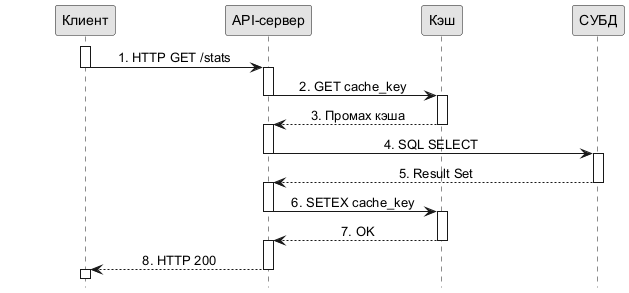
\includegraphics[width=\textwidth]{../img/cache_aside_sequence.png}
\caption{Диаграмма последовательности при паттерне Cache-Aside}
\label{fig:redis-seq}
\end{figure}

Инвалидация кэша выполняется по шаблонам ключей лидербордов, дашборда и данных команд
только для изменённого сезона, а не полным сбросом кэша: это предотвращает
одновременную инвалидацию всех ключей и снижает риск пиковой нагрузки на СУБД
при массовом промахе кэша~--- эффекта «шторма кэша», который
возникает, когда множество параллельных запросов одновременно обнаруживают
истёкший ключ и нагружают базу данных.

\section*{Вывод}

Спроектирована реляционная схема из 8~таблиц, 3~представлений и 6~ключевых индексов;
показано соответствие всех таблиц 1НФ, 2НФ и 3НФ. Бизнес-логика метрик
спроектирована в виде хранимых процедур на стороне СУБД; ограничения целостности закреплены
на уровне ограничений-проверок и триггера. Определена ролевая модель из трёх ролей
с разграничением прав на уровне таблиц, функций и представлений. Спроектировано
REST API из 22~маршрутов, организованных в пять групп и покрывающих все три
варианта использования системы. Для снижения задержки аналитических выборок
спроектировано кэширование по паттерну Cache-Aside с префиксной инвалидацией.

	\chapter{Технологический раздел}

\section{Выбор и обоснование средств реализации}

Профиль нагрузки проектируемой системы сочетает аналитические запросы
на чтение с агрегацией и транзакционную процедуру массового обновления
статистики.

\subsection{СУБД}

Выбор основной СУБД связан с проектными решениями, принятыми в
конструкторском разделе. Расчёт метрик делегирован уровню данных
и реализуется хранимыми функциями в подразделе~\ref{subsec:metric-algorithms},
поэтому требуется процедурный язык на стороне сервера БД. Логическая
проверка командного счёта из раздела~\ref{sec:integrity-design} выполняется
после пакетной загрузки статистики матча, что требует отложенной проверки
целостности к моменту фиксации транзакции. Серверный слой спроектирован
как асинхронный REST API в подразделе~\ref{subsec:app-architecture}, поэтому
взаимодействие с БД не должно блокировать цикл событий приложения. Массовое
обновление сезонной витрины, описанное в подразделе~\ref{subsec:bulk-update},
выполняется одной операцией вставки с обновлением существующих строк.

SQLite~3 является встраиваемой бессерверной СУБД. Такая модель удобна для
локальных приложений и прототипов, но не соответствует серверному сценарию
с несколькими конкурентными подключениями. Кроме того, SQLite не предоставляет
серверный процедурный язык и не имеет штатного асинхронного драйвера для
выбранной модели приложения.

MySQL~8 поддерживает хранимые процедуры и операцию вставки с обновлением.
При этом в рассматриваемом сценарии недостатком является отсутствие
отложенной проверки ограничений целостности к моменту фиксации транзакции.
Это критично для правила, по которому сумма очков игроков должна совпадать
с итоговым счётом команды только после загрузки полного протокола матча.
Также выбранный серверный стек не получает штатного неблокирующего драйвера,
сопоставимого с asyncpg для PostgreSQL.

PostgreSQL~15 удовлетворяет указанным требованиям: поддерживает процедурный
язык PL/pgSQL, отложенную проверку ограничений, атомарную вставку
с обновлением через \texttt{INSERT ... ON CONFLICT DO UPDATE} и работу через
асинхронный драйвер asyncpg~\cite{postgres,asyncpg}. Итоговое сравнение
кандидатов приведено в таблице~\ref{tab:dbms-compare}.

\begin{table}[H]
\caption{Сравнительная характеристика СУБД}
\label{tab:dbms-compare}
\centering
\small
\renewcommand{\arraystretch}{1.2}
\setlength{\tabcolsep}{5pt}
\begin{tabular}{|>{\RaggedRight\arraybackslash}p{0.48\textwidth}
  |>{\centering\arraybackslash}p{0.14\textwidth}
  |>{\centering\arraybackslash}p{0.14\textwidth}
  |>{\centering\arraybackslash}p{0.14\textwidth}|}
\hline
\textbf{Критерий} & \textbf{PostgreSQL 15} & \textbf{MySQL 8} & \textbf{SQLite 3} \\
\hline
Серверный процедурный язык для хранимой логики & Да & Да & Нет \\
\hline
Отложенная проверка ограничений целостности & Да & Нет & Нет \\
\hline
Штатный асинхронный драйвер для выбранного серверного стека & Да & Нет & Нет \\
\hline
Атомарная вставка с обновлением существующей строки & Да & Да & Да \\
\hline
\end{tabular}
\end{table}

По совокупности требований выбрана PostgreSQL~15: она покрывает как
транзакционные механизмы уровня БД, так и интеграцию с асинхронным
серверным приложением.

\subsection{Кэширование}

Паттерн Cache-Aside реализован на базе in-memory СУБД Redis~7~\cite{redis}.
Выбор обоснован поддержкой операций сканирования и группового удаления по
шаблону, что необходимо для инвалидации связанных ключей при пересчёте
статистики отдельного сезона. Команда \texttt{SETEX} позволяет атомарно
устанавливать значение и время жизни ключа, исключая состояние гонки.

\subsection{Серверный слой}

REST API реализован на Python~3.11 с фреймворком FastAPI~\cite{fastapi}.
Фреймворк построен на стандарте ASGI и модели асинхронного ввода-вывода:
каждый обработчик маршрута является корутиной, что позволяет обслуживать
конкурентные запросы в одном процессе без блокировки потока. Механизм
внедрения зависимостей позволяет декларативно привязать к маршруту сессию
конкретной роли СУБД, что соответствует ролевой модели из
раздела~\ref{sec:roles}: разграничение привилегий происходит на уровне
соединения с PostgreSQL, а не в логике приложения. Для взаимодействия с
СУБД применяется драйвер asyncpg~\cite{asyncpg}, реализующий бинарный
протокол PostgreSQL, в связке с SQLAlchemy~2.0 для конструирования
динамических аналитических запросов.

\subsection{Клиентский слой}

Клиентская часть представляет собой одностраничное веб-приложение
на базе библиотеки React~18~\cite{react} и строго типизированного языка
TypeScript. Выбор данного стека технологий обусловлен компонентным подходом
к разработке пользовательского интерфейса, что позволяет эффективно
переиспользовать элементы отображения: таблицы статистики, графики
и карточки игроков. Использование механизма теневого дерева документа
в React обеспечивает высокую производительность при рендеринге объёмных
наборов данных и динамическом обновлении аналитических дашбордов без
полной перезагрузки страницы.

\section{Реализация структуры базы данных}

\subsection{Создание таблиц и ограничений}

Структура базы данных реализована с помощью DDL-скриптов
(полный листинг приведён в Приложении~А). В листинге~\ref{lst:ddl-gps}
представлен фрагмент создания таблицы фактов \texttt{game\_player\_stats},
иллюстрирующий механизм декларативного обеспечения ссылочной и логической
целостности.

\begin{lstlisting}[language=SQL, label=lst:ddl-gps,
  caption=DDL таблицы \texttt{game\_player\_stats} (фрагмент)]
CREATE TABLE game_player_stats (
    stat_id   SERIAL PRIMARY KEY,
    game_id   INTEGER NOT NULL
                REFERENCES games(game_id) ON DELETE CASCADE,
    player_id INTEGER NOT NULL
                REFERENCES players(player_id) ON DELETE RESTRICT,
    team_id   INTEGER NOT NULL
                REFERENCES teams(team_id) ON DELETE RESTRICT,
    points    SMALLINT NOT NULL DEFAULT 0 CHECK (points >= 0),
    fouls     SMALLINT NOT NULL DEFAULT 0 CHECK (fouls BETWEEN 0 AND 6),
    CONSTRAINT uq_game_player UNIQUE (game_id, player_id)
);
\end{lstlisting}

\subsection{Реализация индексов}

Аналитические индексы (Приложение~А) реализованы на базе структуры B-дерева.
В листинге~\ref{lst:indexes} продемонстрировано создание ключевых индексов
для таблицы фактов.

\begin{lstlisting}[language=SQL, label=lst:indexes,
  caption=Создание индексов аналитических запросов (фрагмент)]
CREATE INDEX idx_gps_player_id
    ON game_player_stats(player_id);
CREATE INDEX idx_gps_team_game
    ON game_player_stats(team_id, game_id);
CREATE INDEX idx_pss_season
    ON player_season_stats(season_id, per DESC NULLS LAST);
\end{lstlisting}

Исследование эффективности данных структур и их влияния на время выполнения
запросов приведено в исследовательском разделе (глава~4).

\subsection{Загрузка тестовых данных}\label{subsec:data-load}

Первоначальное наполнение базы данных выполнено средствами языка Python
с использованием библиотеки \texttt{nba\_api}~\cite{nba-api}, формирующей
HTTP-запросы к публично доступным эндпоинтам сервиса
\texttt{stats.nba.com}~\cite{nba-stats}. Скрипт извлекает архивную
статистику NBA за пять регулярных сезонов 2021/22--2025/26.

Полученные данные нормализуются и загружаются в реляционные таблицы
PostgreSQL пакетами в порядке, соответствующем иерархии внешних ключей:
справочники, затем игроки, матчи, статистика матчей, история команд.
Использование официального источника сохраняет репрезентативное распределение
показателей реальных игроков, что критически важно для корректной верификации
относительных метрик.

По результатам контрольных запросов \texttt{SELECT COUNT(*)} объём ключевых
таблиц после загрузки приведён в таблице~\ref{tab:db-count}. Таблица фактов
\texttt{game\_player\_stats} содержит 159\,652 записей, таблица
\texttt{games}~--- 6\,140 матчей. Это полностью покрывает нефункциональное
требование об объёме данных.

{\footnotesize\setlength{\tabcolsep}{4pt}\renewcommand{\arraystretch}{1.15}
\begin{table}[H]
\caption{Объём загруженных данных (контрольный запрос \texttt{SELECT COUNT(*)})}
\label{tab:db-count}
\centering
\begin{tabular}{|l|r|}
\hline
\textbf{Таблица} & \textbf{Число строк} \\
\hline
\texttt{game\_player\_stats}  & 159\,652 \\
\texttt{games}                 & 6\,140 \\
\texttt{players}               & 5\,126 \\
\texttt{player\_season\_stats} & 2\,897 \\
\texttt{teams}                 & 30 \\
\texttt{positions}             & 5 \\
\texttt{seasons}               & 5 \\
\hline
\end{tabular}
\end{table}}

\subsection{Примеры запросов к базе данных}

Для верификации корректности схемы и демонстрации аналитических
возможностей системы разработан набор SQL-запросов, охватывающий основные
классы операций выборки.

Простой запрос с фильтрацией. Выборка активных игроков позиции
центрового. Текст запроса приведён в Приложении~Б,
листинг~\ref{lst:sql-filter}.
Результат выполнения запроса приведён в таблице~\ref{tab:sql-filter-result}.

{\footnotesize\setlength{\tabcolsep}{4pt}\renewcommand{\arraystretch}{1.15}
\begin{table}[H]
\caption{Результат запроса с фильтрацией по позиции центрового}
\label{tab:sql-filter-result}
\centering
\begin{tabular}{|r|l|l|}
\hline
\textbf{ID} & \textbf{Имя} & \textbf{Фамилия} \\
\hline
23  & Steven  & Adams   \\
25  & Bam     & Adebayo \\
61  & Jarrett & Allen   \\
172 & Deandre & Ayton   \\
260 & Charles & Bassey  \\
361 & Goga    & Bitadze \\
363 & Bismack & Biyombo \\
480 & Tony    & Bradley \\
602 & Thomas  & Bryant  \\
694 & Clint   & Capela  \\
\hline
\end{tabular}
\end{table}}

Многотабличный запрос. Получение результатов матчей с названиями
команд и меткой сезона (текст запроса см. в Приложении~Б,
листинг~\ref{lst:sql-join}).
Результат выполнения запроса (первые 10 строк из 1225) приведён
в таблице~\ref{tab:sql-join-result}.

{\footnotesize\setlength{\tabcolsep}{3pt}\renewcommand{\arraystretch}{1.12}
\begin{table}[H]
\caption{Результат многотабличного запроса по матчам сезона 2025-26}
\label{tab:sql-join-result}
\centering
\begin{tabular}{|l|c|l|r|r|l|c|}
\hline
\textbf{Сезон} & \textbf{Дата} & \textbf{Хозяева} & \textbf{Дом.} & \textbf{Гост.} & \textbf{Гости} & \textbf{OT} \\
\hline
2025-26 & 21.10.2025 & Los Angeles Lakers     & 109 & 119 & Golden State Warriors    & 0 \\
2025-26 & 21.10.2025 & Oklahoma City Thunder  & 125 & 124 & Houston Rockets          & 0 \\
2025-26 & 22.10.2025 & Charlotte Hornets      & 136 & 117 & Brooklyn Nets            & 0 \\
2025-26 & 22.10.2025 & Dallas Mavericks       &  92 & 125 & San Antonio Spurs        & 0 \\
2025-26 & 22.10.2025 & Milwaukee Bucks        & 133 & 120 & Washington Wizards       & 0 \\
2025-26 & 22.10.2025 & New York Knicks        & 119 & 111 & Cleveland Cavaliers      & 0 \\
2025-26 & 22.10.2025 & Boston Celtics         & 116 & 117 & Philadelphia 76ers       & 0 \\
2025-26 & 22.10.2025 & Portland Trail Blazers & 114 & 118 & Minnesota Timberwolves   & 0 \\
2025-26 & 22.10.2025 & Utah Jazz              & 129 & 108 & Los Angeles Clippers     & 0 \\
2025-26 & 22.10.2025 & Orlando Magic          & 125 & 121 & Miami Heat               & 0 \\
\hline
\end{tabular}
\end{table}}

Итоговый запрос с агрегацией и группировкой. Средняя
результативность по позициям за сезон, с фильтрацией игроков
с достаточным игровым временем (текст запроса см. в Приложении~Б,
листинг~\ref{lst:sql-group}).
Результат выполнения запроса приведён в таблице~\ref{tab:sql-group-result}.

{\footnotesize\setlength{\tabcolsep}{4pt}\renewcommand{\arraystretch}{1.15}
\begin{table}[H]
\caption{Средняя результативность по позициям (сезон 2025-26)}
\label{tab:sql-group-result}
\centering
\begin{tabular}{|c|r|r|r|r|r|}
\hline
\textbf{Поз.} & \textbf{Игроков} & \textbf{PTS} & \textbf{REB} & \textbf{AST} & \textbf{PER} \\
\hline
C  & 51  & 10.99 & 7.15 & 2.07 & 20.34 \\
PF & 44  & 13.89 & 5.95 & 2.41 & 18.46 \\
PG & 74  & 13.34 & 2.96 & 4.44 & 16.07 \\
SF & 60  & 11.43 & 4.29 & 2.19 & 14.59 \\
SG & 110 & 11.27 & 3.67 & 2.43 & 14.07 \\
\hline
\end{tabular}
\end{table}}

Запрос с подзапросом. Игроки, чей PER превышает среднее
по лиге за сезон (текст запроса см. в Приложении~Б,
листинг~\ref{lst:sql-subquery}).
Результат выполнения запроса (10 строк из 263) приведён
в таблице~\ref{tab:sql-subquery-result}.

{\footnotesize\setlength{\tabcolsep}{4pt}\renewcommand{\arraystretch}{1.15}
\begin{table}[H]
\caption{Игроки с PER выше среднего по лиге (сезон 2025-26)}
\label{tab:sql-subquery-result}
\centering
\begin{tabular}{|l|c|r|r|}
\hline
\textbf{Игрок} & \textbf{Команда} & \textbf{PER} & \textbf{PTS} \\
\hline
Nikola Jokić              & DEN & 37.57 & 27.68 \\
Giannis Antetokounmpo     & MIL & 36.07 & 27.58 \\
Victor Wembanyama         & SAS & 34.58 & 25.05 \\
Shai Gilgeous-Alexander   & OKC & 31.27 & 31.16 \\
Luka Dončić               & LAL & 30.37 & 32.97 \\
Jalen Duren               & DET & 28.65 & 18.25 \\
Kawhi Leonard             & LAC & 28.24 & 27.89 \\
Joel Embiid               & PHI & 26.88 & 26.18 \\
Ty Jerome                 & MEM & 26.52 & 11.80 \\
Jalen Johnson             & ATL & 26.33 & 21.61 \\
\hline
\end{tabular}
\end{table}}

Составной запрос (UNION). Сводный список лидеров по очкам
и передачам в одной выборке (текст запроса см. в Приложении~Б,
листинг~\ref{lst:sql-union}).
Результат выполнения запроса приведён в таблице~\ref{tab:sql-union-result}.

{\footnotesize\setlength{\tabcolsep}{4pt}\renewcommand{\arraystretch}{1.15}
\begin{table}[H]
\caption{Топ-5 лидеров по очкам и передачам (сезон 2025-26)}
\label{tab:sql-union-result}
\centering
\begin{tabular}{|l|l|r|}
\hline
\textbf{Категория} & \textbf{Игрок} & \textbf{Значение} \\
\hline
Scoring & Luka Dončić               & 32.97 \\
Scoring & Shai Gilgeous-Alexander   & 31.16 \\
Scoring & Anthony Edwards           & 28.80 \\
Scoring & Tyrese Maxey              & 28.29 \\
Scoring & Kawhi Leonard             & 27.89 \\
Assists & Nikola Jokić              & 10.72 \\
Assists & Cade Cunningham           &  9.63 \\
Assists & Josh Giddey               &  8.23 \\
Assists & Luka Dončić               &  8.15 \\
Assists & James Harden              &  8.14 \\
\hline
\end{tabular}
\end{table}}

Приведённые запросы охватывают простую фильтрацию, многотабличные
соединения, агрегацию с группировкой, скалярные подзапросы и составные
запросы с объединением результатов.

\section{Реализация логики предметной области в СУБД}

\subsection{Хранимые функции расчёта метрик}

Логика расчёта спортивных метрик реализована в виде хранимых
PL/pgSQL-функций (Приложение~В). Функция \texttt{calculate\_ts}
включает программную защиту от деления на ноль (Приложение~В,
листинг~\ref{lst:ts}).

Все расчётные функции помечены квалификатором \texttt{STABLE}, что позволяет
оптимизатору запросов кэшировать результаты вызовов в рамках одного
оператора. Агрегация сезонной статистики выполняется
хранимой процедурой \texttt{update\_season\_stats} с использованием
атомарной конструкции \texttt{INSERT ... ON CONFLICT DO UPDATE}.

\subsection{Триггеры логической целостности}

Для защиты данных от аномалий используется триггер
\texttt{trg\_check\_team\_score}. Квалификаторы \texttt{DEFERRABLE} и
\texttt{INITIALLY DEFERRED} задают отложенную проверку на этапе
\texttt{COMMIT}. Триггер проверяет бизнес-правило предметной области:
сумма очков всех игроков команды в конкретном матче должна равняться
итоговому командному счёту. Текст функции-триггера приведён
в приложении~В (листинг~\ref{lst:trigger}); команда создания~---
в листинге~\ref{lst:trigger-ddl}.

Триггер \texttt{trigger\_update\_season\_stats} с переходной таблицей
\texttt{inserted\_rows} обеспечивает автоматический пересчёт витрины
\texttt{player\_season\_stats} (листинг~\ref{lst:season-stats-trigger}).

\section{Реализация ролевой модели доступа}

Настройка прав доступа выполнена в соответствии с
принципом минимальных привилегий (Приложение~В, листинг~\ref{lst:grants}).
Роль публичного доступа (\texttt{reader})
лишена возможности прямого обращения к базовым таблицам; чтение
осуществляется исключительно через защищённые представления.

Корректность ограничений для роли \texttt{reader} проверена подключением к БД
от имени пользователя с назначенной ролью \texttt{reader}: запрос \texttt{SELECT * FROM game\_player\_stats} завершился
ошибкой \texttt{permission denied} на уровне PostgreSQL, тогда как
\texttt{SELECT} из представлений \texttt{v\_team\_stats} и \texttt{v\_top\_players},
перечисленных в приложении~В (листинг~\ref{lst:grants}), выполняется успешно.
Аналитические маршруты API, в том числе \texttt{GET /teams/standings},
открывают сессию под ролью \texttt{analyst} и для сводной командной
статистики обращаются к представлению \texttt{v\_team\_stats}.
У роли \texttt{analyst} есть \texttt{SELECT} к базовым таблицам (табл.~\ref{tab:acl-matrix}),
поэтому представления для неё служат удобными витринами, а не единственным
способом чтения данных.

\section{Реализация программного обеспечения и интерфейса}

\subsection{Серверное приложение}

Серверное приложение реализовано в соответствии со спецификацией REST API
конструкторского раздела (подраздел~\ref{subsec:api-spec}). Точкой входа
служит \texttt{app/main.py}, регистрирующий пять групп маршрутов и
CORS-middleware. Подключение к PostgreSQL организовано через три независимых
пула соединений~--- по одному на каждую роль СУБД. Привязка маршрута к
роли осуществляется через аргумент \texttt{Depends};
пример приведён в листинге~\ref{lst:di-role}:

\begin{lstlisting}[language=Python, label=lst:di-role,
  caption=Привязка маршрута к роли СУБД]
@router.get("/leaders")
async def get_leaders(
    season_id: int,
    db: AsyncSession = Depends(get_db_analyst),
    cache: CacheManager = Depends(get_cache),
):
\end{lstlisting}

Маршрут \texttt{/stats/leaders} открывает соединение от имени роли
\texttt{analyst}, имеющей право \texttt{SELECT} к агрегированной статистике
и \texttt{EXECUTE} к функциям расчёта метрик; прямое изменение базовых
таблиц по-прежнему запрещено. Жизненный цикл сессии управляется
генератором: при любом исходе обработчика сессия закрывается,
а незафиксированные изменения откатываются.

\subsection{Кэширование}

Алгоритм паттерна Cache-Aside (класс \texttt{CacheManager}): генерация ключа
на основе параметров, чтение из Redis; при промахе~--- выполнение SQL-запроса,
кэширование результата с установкой времени жизни (TTL) и возврат ответа.
Пример для маршрута \texttt{/stats/leaders} приведён в листинге~\ref{lst:cache-aside-pattern};
обобщённый вариант декоратора Cache-Aside~--- в Приложении~Г.

\begin{lstlisting}[language=Python, label=lst:cache-aside-pattern,
  caption=Cache-Aside в маршруте \texttt{/stats/leaders}]
cache_key = (
    f"leaders:{metric}:{season_id}:{team_id}:{position}:{min_games}:{limit}"
)
cached = await cache.get(cache_key)
if cached:
    return cached
result = await db.execute(query)
data = [...]
await cache.set(cache_key, data, ttl=900)
return data
\end{lstlisting}

Время жизни ключей дифференцировано по типу данных: данные завершённых
матчей кэшируются на один год, лидерборды и списки составов команд~---
на 15 минут,
результаты поиска~--- на 2 минуты. Инвалидация при вызове
\texttt{POST /admin/refresh/\{season\_id\}} выполняется по шаблонам ключей
затронутого сезона в соответствии с проектным решением
подраздела~\ref{subsec:cache}.

\subsection{Пользовательский интерфейс}

Интеграция библиотеки Recharts~\cite{recharts} обеспечивает рендеринг
диаграмм и графиков трендов.

Навигация включает аналитический дашборд с KPI-метриками лиги, таблицу
игроков с серверной фильтрацией, турнирные сводки конференций, глобальный
рейтинг лидеров и раздел расширенной статистики с диаграммами рассеяния
(рисунок~\ref{fig:ui-dashboard}). По выбору строки открывается модальное окно
профиля с сезонными метриками и игровым журналом (рисунок~\ref{fig:ui-modal}).
Модуль сравнения двух игроков реализован в виде модального окна
с радарным графиком, гистограммой базовой статистики и цветовым выделением
превосходящих метрик (рисунок~\ref{fig:ui-compare}).

\section{Тестирование и верификация аналитических данных}

Тестирование логики СУБД проводилось методом чёрного ящика. Для проверки
точности математических агрегаций выполнен регрессионный тест на реальных
данных из загруженной базы: эталонные значения получены независимым
расчётом по формулам раздела~1.2, после чего сопоставлены с результатами
хранимых функций PostgreSQL.

В качестве тестового объекта выбран профиль игрока Nikola Joki\'{c}
с идентификатором~2327 за регулярный сезон 2025-26 с идентификатором~5.
Прямой SQL-запрос суммы сырых фактов из таблицы
\texttt{game\_player\_stats} вернул следующие значения:
\begin{itemize}
    \item очки: 1799;
    \item броски с игры: 1132;
    \item штрафные попытки: 480.
\end{itemize}

Ручной расчёт истинного процента бросков по формуле~(\ref{eq:ts}):
\[
\mathrm{TS\%} = \frac{1799}{2 \cdot (1132 + 0{,}44 \cdot 480)}
  = \frac{1799}{2686{,}4} \approx 0{,}6697.
\]

Для верификации в СУБД выполнен вызов хранимой функции:
\begin{lstlisting}[language=SQL]
SELECT calculate_ts(2327, 5);
\end{lstlisting}

Результат совпал с ручным расчётом. Аналогичная верификация проведена для
eFG\% и USG\%; расхождений не выявлено.

Верификация PER выполнена по той же методике. Из таблицы
\texttt{game\_player\_stats} получены сезонные суммы для
\texttt{player\_id = 2327}: $\mathrm{PTS} = 1799$, $\mathrm{TRB} = 836$,
$\mathrm{AST} = 697$, $\mathrm{STL} = 92$, $\mathrm{BLK} = 53$,
$\mathrm{TOV} = 243$, $\mathrm{PF} = 173$, $\mathrm{FGM/FGA} = 644/1132$,
$\mathrm{FTM/FTA} = 399/480$, $\mathrm{MP} = 2264{,}8$.
Ненормализованный вклад по формуле uPER (раздел~1.2):
\[
\mathrm{uPER} =
(1799 + 836 + 697 + 92 + 53 - 243 - 173 - 488 - 35{,}64)
\cdot \frac{48}{2264{,}8} = 2537{,}36 \cdot \frac{48}{2264{,}8}
\approx 53{,}78.
\]
Лиговое среднее по формуле~(1.5) по 503~игрокам с $\mathrm{MP} > 100$:
$\mathrm{lg\_aPER} = 21{,}47$. Итоговый рейтинг по формуле~(1.6):
\[
\mathrm{PER} = 53{,}78 \cdot \frac{15}{21{,}47} \approx 37{,}57.
\]
Вызов \texttt{SELECT calculate\_per(2327, 5)} вернул $37{,}57$~---
расхождений не выявлено.

Тестирование граничных случаев подтвердило корректный возврат значения
\texttt{NULL} при отсутствии попыток бросков и нулевом времени на площадке.
Работа триггера \newline\texttt{trg\_check\_team\_score} проверена попыткой вставки
в одной транзакции строк с намеренно неверной суммой очков: при
\texttt{COMMIT} триггер поднял исключение
\texttt{Player points sum does not match team score}, транзакция была
отклонена~--- поведение соответствует ожидаемому
(таблица~\ref{tab:test-cases}).

{\footnotesize\setlength{\tabcolsep}{3pt}\renewcommand{\arraystretch}{1.2}
\begin{table}[H]
\caption{Контрольные тест-кейсы функций расчёта метрик}
\label{tab:test-cases}
\centering
\begin{tabular}{|c|p{0.24\textwidth}|p{0.27\textwidth}|p{0.17\textwidth}|p{0.14\textwidth}|}
\hline
\textbf{№} & \textbf{Сценарий} & \textbf{Входные данные}
  & \textbf{Ожидание} & \textbf{Результат} \\
\hline
1 & Нормальный профиль & \texttt{calculate\_ts(2327, 5)}
  & $\approx 0{,}6697$ & совпало \\
\hline
2 & Нет попыток броска & \texttt{calculate\_ts(0, 0)}
  & NULL & NULL \\
\hline
3 & Нулевые FGA (eFG\%) & \texttt{calculate\_efg(0, 0)}
  & NULL & NULL \\
\hline
4 & Пересчёт витрины & \texttt{CALL update\_season\_stats(5)}
  & обновлены строки \texttt{pss} & выполнено \\
\hline
5 & Верификация PER & \texttt{calculate\_per(2327, 5)}
  & $\approx 37{,}57$ (формулы 1.4--1.6) & 37{,}57, совпало \\
\hline
6 & Триггер целостности счёта & INSERT с суммой очков,
  не совпадающей с \texttt{home\_score}
  & EXCEPTION при попытке фиксации транзакции (COMMIT) & исключение при COMMIT,
  транзакция отклонена \\
\hline
\end{tabular}
\end{table}
}

Для формализации тестового покрытия каждой функции на стороне СУБД
выделены классы эквивалентности~--- непересекающиеся разделы входных
данных, для которых ожидается одинаковое поведение функции. Разбиение
приведено в таблице~\ref{tab:eq-classes}.

\begin{table}[H]
\caption{Классы эквивалентности функций на стороне СУБД}
\label{tab:eq-classes}
\centering
\begin{tabular}{|>{\raggedright\arraybackslash}p{0.21\textwidth}|c|>{\raggedright\arraybackslash}p{0.28\textwidth}|>{\raggedright\arraybackslash}p{0.22\textwidth}|>{\raggedright\arraybackslash}p{0.14\textwidth}|}
\hline
\textbf{Функция} & \textbf{КЭ} & \textbf{Условие раздела} & \textbf{Представитель} & \textbf{Ожидание} \\
\hline

\texttt{calculate\_efg}
 & КЭ1 & FGA $> 0$, FG3M $\geq 0$ & \texttt{calc\_efg(2327, 5)} & $\in (0; 1]$ \\
 & КЭ2 & FGA $= 0$ (нет бросков) & \texttt{calc\_efg(0, 0)} & NULL \\
 & КЭ3 & team\_id IS NULL (агрегация по всем командам) & \texttt{calc\_efg(2327, 5, NULL)} & $=$ КЭ1 \\
\hline
\texttt{calculate\_usg}
 & КЭ1 & MP $\geq 1$, denom $> 0$ & \texttt{calc\_usg(2327, 5)} & $\in (0; 1]$ \\
 & КЭ2 & MP $< 1$ (игрок не выходил) & несуществующий player\_id & NULL \\
 & КЭ3 & командный знаменатель $= 0$ & аномальные тестовые данные & NULL \\
 & КЭ4 & team\_id не определён (нет матчей) & несуществующий player\_id & NULL \\
\hline
\texttt{calculate\_ts}
 & КЭ1 & FGA $> 0$ или FTA $> 0$ & \texttt{calc\_ts(2327, 5)} & $\approx 0{,}6697$ \\
 & КЭ2 & FGA $= 0$ и FTA $= 0$ & \texttt{calc\_ts(0, 0)} & NULL \\
 & КЭ3 & знаменатель $= 0$ при FGA $= 0$, FTA $> 0$ (редкий) & аномальные тестовые данные & NULL \\
\hline
\texttt{calculate\_per}
 & КЭ1 & MP $\geq 50$, lg\_aPER $> 0$ & \texttt{calc\_per(2327, 5)} & $\approx 37{,}57$ \\
 & КЭ2 & MP $< 50$ (дисквалифицирован) & игрок с малым числом игр & NULL \\
 & КЭ3 & lg\_aPER $= 0$ или NULL (пустой сезон) & фиктивный season\_id без данных & нормировка на $15{,}0$ \\
\hline
\texttt{calculate\_bpm}
 & КЭ1 & MP $\geq 50$ & \texttt{calc\_bpm(2327, 5)} & числовое значение \\
 & КЭ2 & MP $< 50$ & игрок с малым числом игр & NULL \\
\hline
\texttt{trg\_validate\_} \texttt{team\_score\_row}
 & КЭ1 & статус $\neq$ \texttt{Finished} или счёт NULL & INSERT в незавершённый матч & принято без проверки \\
 & КЭ2 & статус \texttt{Finished}, $\sum\mathrm{points} =$ счёт & корректный INSERT & принято \\
 & КЭ3 & статус \texttt{Finished}, $\sum\mathrm{points} \neq$ счёт & INSERT с неверной суммой очков & EXCEPTION \\
\hline
\texttt{trigger\_update\_} \texttt{season\_stats}
 & КЭ1 & season\_id найден & штатный INSERT в \texttt{game\_player\_stats} & вызов \texttt{update\_} \texttt{season\_} \texttt{stats} \\
 & КЭ2 & season\_id IS NULL (пустая таблица) & таблица без строк & возврат NULL без вызова \\
\hline
\end{tabular}
\end{table}

Тестирование выполнено по всем выделенным классам эквивалентности.
Для каждого класса фактическое поведение функции совпало с ожидаемым:
корректные входные данные дают значения в допустимом диапазоне, граничные
и вырожденные случаи возвращают NULL либо предусмотренную нормировку,
а нарушение бизнес-правила счёта вызывает исключение на этапе фиксации
транзакции. Все тесты пройдены успешно, расхождений не выявлено.

\section*{Вывод}

В технологическом разделе обоснован стек технологий (PostgreSQL~15,
Redis~7, FastAPI, React~18) и реализована структура базы данных средствами
DDL: таблицы, ограничения целостности и индексы.
Разработаны PL/pgSQL-функции и триггеры, обеспечивающие расчёт метрик и
консистентность данных. С помощью написанного ETL-скрипта БД наполнена
реальной статистикой NBA (более 150~тыс. фактов). Успешно реализованы
механизмы кэширования (Cache-Aside) и ролевого доступа. Регрессионное
тестирование на реальных данных подтвердило математическую корректность
работы базы данных и хранимых процедур.
	\chapter{Исследовательский раздел}

\section{Цель и методика исследования}

Целью раздела является оценка производительности аналитических запросов
при изменении объёма данных, конфигурации индексов, состояния кэша и уровня
параллельной нагрузки. Измерения выполняются для ключевых механизмов системы:
предвычисленной витрины \texttt{player\_season\_stats}, индексов B-tree,
Redis-кэша и асинхронного API-сервера.

Замеры автоматизированы Python-скриптом: SQL-запросы выполняются через
asyncpg, HTTP-запросы к API~--- через httpx. PostgreSQL~15, Redis~7
и API-сервер развёрнуты в Docker-контейнерах на одном хосте:
CPU~--- Intel Core i5-1235U (10~ядер, 3{,}3~ГГц), ОЗУ~--- 16~ГБ DDR4,
хранилище~--- NVMe SSD. Таблица фактов \texttt{game\_player\_stats}
содержит 159\,652~строк за пять сезонов NBA.

Для SQL-запросов выполнялось 10~прогревочных запусков и 10\,000~рабочих
повторов. По рабочим замерам рассчитывались медиана, среднее значение
и 95-й перцентиль. Выбросы отдельно не отсекались. Для проверки кэширования
измерялись Cache Miss (30~запросов со сбросом кэша перед каждым запросом)
и Cache Hit (10\,000~запросов после прогрева кэша). Нагрузочные замеры выполнены
для 1, 10, 50 и 100~параллельных запросов, по 10~раундов на каждый уровень.
Ошибкой считается HTTP-код не ниже 500, таймаут или отказ соединения.

\section{Влияние объёма данных на производительность}

Для оценки влияния объёма данных сопоставлены два способа получения рейтинга
лидеров: прямая агрегация по таблице фактов и выборка из предвычисленной
витрины. Объём изменялся накопительно: от одного сезона до пяти сезонов.
Эффект витрины оценивается кратностью ускорения~--- отношением медианного
времени прямой агрегации к медианному времени выборки из витрины на одном
и том же наборе сезонов.

Запрос прямой агрегации по таблице фактов приведён
в листинге~\ref{lst:research-heavy-agg}.

\begin{lstlisting}[language=SQL, label=lst:research-heavy-agg,
  caption=Прямой агрегирующий запрос к таблице фактов]
SELECT gps.player_id,
       SUM(gps.points)        AS total_pts,
       COUNT(*)               AS games,
       AVG(gps.points::float) AS avg_pts
FROM game_player_stats gps
JOIN games g ON g.game_id = gps.game_id
WHERE g.season_id = ANY($1::int[])
GROUP BY gps.player_id
ORDER BY total_pts DESC
LIMIT 20;
\end{lstlisting}

Запрос к предвычисленной витрине приведён
в листинге~\ref{lst:research-vitrina-query}.

\begin{lstlisting}[language=SQL, label=lst:research-vitrina-query,
  caption=Запрос к предвычисленной витрине]
SELECT player_id, season_id, per, avg_pts
FROM player_season_stats
WHERE season_id = ANY($1::int[])
ORDER BY per DESC NULLS LAST
LIMIT 20;
\end{lstlisting}

Результаты замеров приведены в таблице~\ref{tab:volume-fact-vitrina}.

\begin{table}[H]
\caption{Влияние объёма данных на прямую агрегацию и выборку из витрины}
\label{tab:volume-fact-vitrina}
\centering
\small
\begin{tabular}{|p{0.13\textwidth}|p{0.16\textwidth}|p{0.16\textwidth}
  |p{0.16\textwidth}|p{0.16\textwidth}|p{0.16\textwidth}|}
\hline
\textbf{Сезоны} & \textbf{Строк фактов} & \textbf{Строк витрины}
  & \textbf{Агрегация, медиана (мс)} & \textbf{Витрина, медиана (мс)}
  & \textbf{Ускорение, раз} \\
\hline
1       & 31\,311  & 586   & 18{,}58 & 0{,}44 & 42{,}2 \\
\hline
1--2    & 62\,853  & 1\,140 & 24{,}75 & 0{,}66 & 37{,}5 \\
\hline
1--3    & 95\,235  & 1\,721 & 25{,}25 & 0{,}78 & 32{,}4 \\
\hline
1--4    & 127\,607 & 2\,304 & 29{,}09 & 0{,}90 & 32{,}3 \\
\hline
1--5    & 159\,652 & 2\,897 & 35{,}58 & 1{,}15 & 30{,}9 \\
\hline
\end{tabular}
\end{table}

Зависимость медианного времени выполнения от объёма данных показана
на рисунке~\ref{fig:volume-fact-vitrina}.

\begin{figure}[H]
\centering
\begin{tikzpicture}
\begin{axis}[
    width=0.88\textwidth,
    height=6.5cm,
    xlabel={Количество строк фактов},
    ylabel={Медианное время выполнения (мс)},
    xmin=25000, xmax=165000,
    ymin=0, ymax=38,
    scaled x ticks=false,
    xtick={31311,62853,95235,127607,159652},
    xticklabels={31\,311,62\,853,95\,235,127\,607,159\,652},
    x tick label style={font=\scriptsize, rotate=25, anchor=east},
    ymajorgrids=true,
    grid style=dashed,
    legend style={
      at={(0.5,1.14)},
      anchor=south,
      legend columns=2,
      font=\small,
      draw=none
    },
    mark size=3pt,
]
\addplot+[mark=*, thick, color=black] coordinates {
    (31311, 18.58)
    (62853, 24.75)
    (95235, 25.25)
    (127607, 29.09)
    (159652, 35.58)
};
\addplot+[mark=square*, thick, color=black, dashed] coordinates {
    (31311, 0.44)
    (62853, 0.66)
    (95235, 0.78)
    (127607, 0.90)
    (159652, 1.15)
};
\legend{Прямая агрегация, Витрина}
\end{axis}
\end{tikzpicture}
\caption{Влияние объёма данных на время аналитической выборки}
\label{fig:volume-fact-vitrina}
\end{figure}

При росте таблицы фактов с 31\,311 до 159\,652~строк медиана прямой
агрегации увеличилась с 18{,}58 до 35{,}58~мс. Запрос к витрине выполняется
за 0{,}44--1{,}15~мс, поскольку использует готовые сезонные агрегаты.
На полном объёме данных витрина ускоряет выборку примерно в 31~раз.

Кратность ускорения максимальна на одном сезоне (42{,}2~раза) и плавно
снижается к пяти сезонам. Причина~--- в устройстве кумулятивного запроса
к витрине: одиночный сезон обслуживается одним диапазонным сканом индекса,
тогда как \texttt{season\_id = ANY(...)} сканирует несколько диапазонов
и пересортировывает строки по \texttt{per} через все сезоны. Из-за этих
накладных расходов время витрины с ростом числа сезонов увеличивается
пропорционально быстрее времени агрегации (в абсолютных величинах витрина
остаётся быстрее в десятки раз), поэтому кратность ускорения убывает,
оставаясь в пределах 31--42~раз.

\section{Влияние индексирования на селективную выборку}

Влияние индексов оценивалось на селективной выборке~--- получении полного
игрового лога одного игрока (листинг~\ref{lst:research-player-log}). Запрос
фильтрует таблицу фактов по \texttt{player\_id} и возвращает 410~строк
из 159\,652, то есть 0{,}26\,\% объёма. Индекс \texttt{idx\_gps\_player\_id}
спроектирован в подразделе~\ref{subsec:indexes}; его DDL-объявление приведено
в листинге~\ref{lst:indexes} и Приложении~А.

\begin{lstlisting}[language=SQL, label=lst:research-player-log,
  caption=Селективная выборка игрового лога игрока]
SELECT gps.game_id, gps.points, gps.assists,
       gps.rebounds_off, gps.rebounds_def
FROM game_player_stats gps
WHERE gps.player_id = $1
ORDER BY gps.game_id;
\end{lstlisting}

Сравнивались две конфигурации: выполнение без индекса по фильтруемому
столбцу (последовательный просмотр таблицы) и с индексом
\texttt{idx\_gps\_player\_id}. Результаты приведены
в таблице~\ref{tab:fact-indexes}.

\begin{table}[H]
\caption{Влияние индекса по столбцу фильтрации на селективную выборку}
\label{tab:fact-indexes}
\centering
\small
\begin{tabular}{|p{0.40\textwidth}|p{0.14\textwidth}|p{0.14\textwidth}|p{0.14\textwidth}|}
\hline
\textbf{Конфигурация} & \textbf{Медиана (мс)}
  & \textbf{Среднее (мс)} & \textbf{P95 (мс)} \\
\hline
Без индекса (Seq Scan) & 13{,}05 & 17{,}99 & 48{,}74 \\
\hline
\texttt{idx\_gps\_player\_id} (Bitmap Index Scan) & 2{,}46 & 3{,}44 & 11{,}08 \\
\hline
\end{tabular}
\end{table}

Сравнение времени выполнения без индекса и с индексом показано
на рисунке~\ref{fig:fact-indexes}.

\begin{figure}[H]
\centering
\begin{tikzpicture}
\begin{axis}[
    ybar,
    bar width=26pt,
    width=0.88\textwidth,
    height=6.6cm,
    ylabel={Время выполнения (мс)},
    symbolic x coords={Без индекса, С индексом},
    xtick=data,
    x tick label style={font=\small},
    enlarge x limits=1.2,
    ymin=0, ymax=56,
    ytick={0,10,20,30,40,50},
    ymajorgrids=true,
    grid style=dashed,
    nodes near coords,
    nodes near coords style={font=\scriptsize,
      /pgf/number format/fixed,
      /pgf/number format/precision=2},
    every node near coord/.append style={anchor=south, yshift=1pt},
    legend style={at={(0.5,1.10)}, anchor=south, legend columns=2,
      font=\small, draw=none},
]
\addplot+[fill=white, draw=black,
          postaction={pattern=north east lines}] coordinates {
    (Без индекса, 13.05)
    (С индексом, 2.46)
};
\addplot+[fill=black!15, draw=black] coordinates {
    (Без индекса, 48.74)
    (С индексом, 11.08)
};
\legend{Медиана, P95}
\end{axis}
\end{tikzpicture}
\caption{Время селективной выборки без индекса и с индексом по игроку}
\label{fig:fact-indexes}
\end{figure}

Без индекса выборка выполняется последовательным просмотром: СУБД читает
все 159\,652~строки таблицы фактов и отбрасывает 159\,242~из них,
не удовлетворяющие условию по \texttt{player\_id}. Индекс
\texttt{idx\_gps\_player\_id} переводит запрос на доступ по индексу
(Bitmap Index Scan), при котором читаются только 410~релевантных строк.
Медианное время снижается с 13{,}05 до 2{,}46~мс, P95~--- с 48{,}74
до 11{,}08~мс, что соответствует ускорению примерно в 5{,}3~раза.

\section{Влияние кэширования}

Кэширование проверялось на маршруте \texttt{/stats/leaders} с параметрами
\texttt{metric=per}, \texttt{season\_id=5} и \texttt{limit=20}. В сценарии
Cache Miss перед каждым запросом удалялись ключи лидерборда. В сценарии
Cache Hit кэш предварительно прогревался.

Результаты сравнения приведены в таблице~\ref{tab:cache-effect}.

\begin{table}[H]
\caption{Время ответа API при холодном и тёплом кэше}
\label{tab:cache-effect}
\centering
\small
\begin{tabular}{|p{0.30\textwidth}|p{0.18\textwidth}|p{0.18\textwidth}|p{0.18\textwidth}|}
\hline
\textbf{Сценарий} & \textbf{Медиана (мс)}
  & \textbf{Среднее (мс)} & \textbf{P95 (мс)} \\
\hline
Cache Miss, PostgreSQL & 11{,}68 & 11{,}76 & 15{,}50 \\
\hline
Cache Hit, Redis & 3{,}69 & 4{,}66 & 11{,}57 \\
\hline
\end{tabular}
\end{table}

При Cache Hit медиана ответа снижается с 11{,}68 до 3{,}69~мс,
P95~--- с 15{,}50 до 11{,}57~мс. Ускорение составляет примерно 3{,}2~раза:
API читает готовый JSON из Redis и не выполняет SQL-запрос.

\section{Влияние уровня нагрузки}

Нагрузочное исследование выполнялось для маршрута \texttt{/stats/leaders}
с параметрами \texttt{metric=per}, \texttt{season\_id=5} и \texttt{limit=20}.
Перед каждым раундом выполнялся прогревочный запрос, поэтому замеры отражают
работу API при тёплом Redis-кэше. Обращение без кэша рассмотрено отдельно
в разделе~4.4.

Результаты нагрузочного тестирования приведены в таблице~\ref{tab:load-warm}.

\begin{table}[H]
\caption{Время ответа API при параллельной нагрузке}
\label{tab:load-warm}
\centering
\small
\begin{tabular}{|p{0.24\textwidth}|p{0.16\textwidth}|p{0.16\textwidth}
  |p{0.16\textwidth}|p{0.16\textwidth}|}
\hline
\textbf{Параллельных запросов} & \textbf{Медиана (мс)}
  & \textbf{Среднее (мс)} & \textbf{P95 (мс)} & \textbf{Ошибки (\%)} \\
\hline
1   & 3{,}25   & 3{,}64   & 6{,}62   & 0 \\
\hline
10  & 16{,}43  & 17{,}20  & 32{,}21  & 0 \\
\hline
50  & 71{,}00  & 78{,}61  & 139{,}82 & 0 \\
\hline
100 & 252{,}14 & 326{,}10 & 821{,}08 & 0 \\
\hline
\end{tabular}
\end{table}

Зависимость времени ответа от числа параллельных запросов показана
на рисунке~\ref{fig:load-warm}.

\begin{figure}[H]
\centering
\begin{tikzpicture}
\begin{axis}[
    width=0.88\textwidth,
    height=6.8cm,
    xlabel={Число параллельных запросов},
    ylabel={Время ответа API (мс)},
    xmode=log,
    log basis x=10,
    xtick={1,10,50,100},
    xticklabels={1,10,50,100},
    ymin=0, ymax=860,
    ymajorgrids=true,
    grid style=dashed,
    legend style={
      at={(0.5,1.14)},
      anchor=south,
      legend columns=3,
      font=\small,
      draw=none
    },
    mark size=3pt,
]
\addplot+[mark=*, thick, color=black] coordinates {
    (1, 3.64)
    (10, 17.20)
    (50, 78.61)
    (100, 326.10)
};
\addplot+[mark=square*, thick, color=black, dashed] coordinates {
    (1, 6.62)
    (10, 32.21)
    (50, 139.82)
    (100, 821.08)
};
\addplot+[mark=none, thick, color=black, dotted] coordinates {
    (1, 100) (100, 100)
};
\legend{Среднее время, P95, Требование 100\,мс}
\end{axis}
\end{tikzpicture}
\caption{Время ответа API при росте параллельной нагрузки}
\label{fig:load-warm}
\end{figure}

При нагрузке до 10~запросов P95 (32{,}21~мс) укладывается в требование 100~мс.
При пиковой нагрузке в 100~подключений показатели времени ответа превышают
требования из-за исчерпания пула соединений, однако система сохраняет
отказоустойчивость. Деградация обусловлена насыщением пула соединений
с PostgreSQL и очереди event loop единственного экземпляра Uvicorn.

\section{Анализ результатов и рекомендации}

\textbf{1. Предвычисленная витрина снижает стоимость аналитических выборок.}

На полном объёме прямая агрегация занимает 35{,}58~мс, выборка из витрины~---
1{,}15~мс. Предварительный расчёт сезонных агрегатов уменьшает время
аналитического запроса примерно в 31~раз.

\textbf{2. Индекс по столбцу фильтрации ускоряет селективные выборки.}

Для выборки игрового лога одного игрока индекс \texttt{idx\_gps\_player\_id}
переводит запрос с последовательного просмотра на доступ по индексу
и снижает медианное время примерно в 5{,}3~раза (с 13{,}05 до 2{,}46~мс).

\textbf{3. Redis-кэш снижает задержку одиночных аналитических запросов.}

Переход от Cache Miss к Cache Hit уменьшает медиану ответа с 11{,}68
до 3{,}69~мс и P95 с 15{,}50 до 11{,}57~мс. Кэш следует применять для
повторяющихся рейтингов и дашбордов.

\textbf{4. Порог устойчивой параллельной нагрузки находится между 10 и 50 запросами.}

При 10~одновременных запросах P95 составляет 32{,}21~мс. При 50~запросах
P95 превышает 100~мс (139{,}82~мс), хотя медиана остаётся равной 71{,}00~мс. Для пиковых
нагрузок требуется масштабирование API-сервера: несколько worker-процессов,
балансировщик и общий Redis-кэш.

\section*{Вывод}

Предвычисленная витрина ускоряет аналитические выборки примерно в 31~раз
на полном объёме данных. Индекс \texttt{idx\_gps\_player\_id} ускоряет
селективную выборку по игроку примерно в 5{,}3~раза. Redis-кэш уменьшает
медианную задержку API примерно в 3{,}2~раза. При параллельной нагрузке система не возвращает ошибок,
но требование P95 менее 100~мс выполняется до 10~одновременных запросов
включительно; для большей нагрузки требуется масштабирование API-уровня.


	\chapter*{ЗАКЛЮЧЕНИЕ}
\addcontentsline{toc}{chapter}{ЗАКЛЮЧЕНИЕ}

В рамках выполнения курсовой работы была успешно спроектирована
и реализована база данных для хранения и анализа спортивной статистики.
Поставленная цель достигнута в полном объёме посредством решения
сформулированных задач:
\begin{enumerate}
    \item выполнен сравнительный анализ предметной области, сформулированы требования
          и ограничения к системе. Определен перечень метрик и формализована
          математическая методология их расчета. Выделены ключевые сущности и роли,
          построены диаграммы вариантов использования и диаграмма сущность-связь, выбрана
          реляционная модель данных;
    \item спроектирована структура базы данных в третьей нормальной форме. Разработаны
          алгоритмы автоматизированной обработки и расчёта аналитических показателей.
          Спроектированы ролевая модель доступа на уровне СУБД, серверное программное
          обеспечение для взаимодействия с БД и подсистема кэширования
          с префиксной инвалидацией ключей;
    \item обоснован выбор средств реализации, реализована структура базы данных
          средствами DDL и серверное приложение, предоставляющее API из двадцати двух
          маршрутов. Подготовлен набор тестовых данных объемом более ста пятидесяти
          тысяч фактов. Выполнено тестирование системы, доказавшее корректность
          работы и математическую точность расчёта показателей;
    \item проведено исследование влияния объема данных, стратегий индексации
          и уровня нагрузки на производительность выполнения аналитических запросов.
          Доказано, что применение целевых одиночных индексов сокращает среднее время
          выполнения аналитических выборок
          на~50\% и радикально снижает 95-й перцентиль задержки. Обращение
          к предвычисленной витрине ускоряет получение данных примерно в~31{,}5~раза
          по сравнению с прямой агрегацией, а использование in-memory кэширования
          снижает медианное время ответа сервера в~3{,}9~раза. На основе полученных
          результатов сформулированы рекомендации по оптимизации и масштабированию
          системы при росте конкурентной нагрузки.
\end{enumerate}

Разработанный программный комплекс представляет собой готовое
масштабируемое решение, применимое для обеспечения деятельности
аналитических отделов спортивных организаций.


	\def\bibname{\begin{center}\Large СПИСОК ИСПОЛЬЗОВАННЫХ ИСТОЧНИКОВ\end{center}}
	\begin{thebibliography}{99}

	\addcontentsline{toc}{chapter}{СПИСОК ИСПОЛЬЗОВАННЫХ ИСТОЧНИКОВ}

	\bibitem{nba-stats}
	NBA Stats [Электронный ресурс]. — Официальная статистика Национальной баскетбольной ассоциации. — Режим доступа: \url{https://www.nba.com/stats} (дата обращения: 29.03.2026).

	\bibitem{glossary-nba}
	Glossary --- NBA.com : Stats [Электронный ресурс]. — Термины и определения показателей (в т.\,ч. eFG\%, TS\%). — Режим доступа: \url{https://www.nba.com/stats/help/glossary} (дата обращения: 29.03.2026).

	\bibitem{bref}
	Basketball-Reference.com [Электронный ресурс]. — Sports Reference LLC. Справочник статистики NBA и исторические таблицы. — Режим доступа: \url{https://www.basketball-reference.com/} (дата обращения: 29.03.2026).

	\bibitem{per-bref}
	Player Efficiency Rating [Электронный ресурс] // Basketball-Reference.com. — Описание показателя PER (Дж. Холлинджер). — Режим доступа: \url{https://www.basketball-reference.com/about/per.html} (дата обращения: 29.03.2026).

	\bibitem{bpm-bref}
	BPM (Box Plus/Minus) [Электронный ресурс] // Basketball-Reference.com. — Описание показателя BPM. — Режим доступа: \url{https://www.basketball-reference.com/about/bpm2.html} (дата обращения: 29.03.2026).

	\bibitem{espn}
	ESPN NBA [Электронный ресурс]. — Новости и обзоры НБА (справочно о медиа-формате представления статистики). — Режим доступа: \url{https://www.espn.com/nba/} (дата обращения: 29.03.2026).

	\bibitem{connolly}
	Коннолли, Т. Базы данных. Проектирование, реализация и сопровождение. Теория и практика / Т. Коннолли, К. Бегг ; пер. с англ. — 3-е изд. — М. : Вильямс, 2003. — 1440 с.

	\bibitem{chen}
	Chen, P. P. The Entity-Relationship Model --- Toward a Unified View of Data / P. P. Chen // ACM Transactions on Database Systems. --- 1976. --- Vol.~1, №~1. --- P.~9--36.

	\bibitem{date}
	Дейт, К. Дж. Введение в системы баз данных / К. Дж. Дейт ; пер. с англ. — 8-е изд. — М. : Вильямс, 2006. — 1328 с.

	\bibitem{redis}
	Redis Documentation [Электронный ресурс]. — Документация in-memory хранилища Redis. — Режим доступа: \url{https://redis.io/docs/} (дата обращения: 29.03.2026).

	\bibitem{postgres}
	PostgreSQL 15 Documentation [Электронный ресурс]. — Официальная документация СУБД PostgreSQL. — Режим доступа: \url{https://www.postgresql.org/docs/15/} (дата обращения: 29.03.2026).

	\bibitem{python}
	Python 3 Documentation [Электронный ресурс]. — Официальная документация языка программирования Python. — Режим доступа: \url{https://docs.python.org/3/} (дата обращения: 29.03.2026).

	\bibitem{fastapi}
	FastAPI [Электронный ресурс]. — Официальная документация веб-фреймворка FastAPI. — Режим доступа: \url{https://fastapi.tiangolo.com/} (дата обращения: 29.03.2026).

	\bibitem{react}
	React Documentation [Электронный ресурс]. — Официальная документация библиотеки React. — Режим доступа: \url{https://react.dev/} (дата обращения: 29.03.2026).

\end{thebibliography}


	\chapter*{ПРИЛОЖЕНИЯ}
\addcontentsline{toc}{chapter}{ПРИЛОЖЕНИЯ}

\section*{Приложение А. Блок-схемы алгоритмов}
\addcontentsline{toc}{section}{Приложение А. Блок-схемы алгоритмов}

\renewcommand{\thefigure}{А.\arabic{figure}}
\setcounter{figure}{0}
\begin{figure}[H]
\centering
\begin{tikzpicture}[
    node distance=1.5cm,
    every node/.style={font=\footnotesize},
    startstop/.style={draw, rectangle, rounded corners=10pt, minimum width=3.2cm,
      minimum height=0.8cm, align=center, fill=white},
    process/.style={draw, rectangle, minimum width=3.2cm, minimum height=0.9cm,
      align=center, fill=white},
    io/.style={draw, trapezium, trapezium left angle=75, trapezium right angle=105,
      trapezium stretches=true, minimum width=3.5cm, minimum height=0.8cm,
      align=center, fill=white},
    decision/.style={draw, diamond, aspect=2.5, minimum width=3cm,
      minimum height=0.8cm, align=center, fill=white},
    arrow/.style={thick,->,>=stealth}
]
\node (start)  [startstop] {Начало};
\node (pro1)   [process,  below of=start] {Суммирование PTS, FGA, FTA};
\node (pro2)   [process,  below of=pro1]
  {$D = 2 \cdot (\mathrm{FGA} + 0{,}44 \cdot \mathrm{FTA})$};
\node (dec1)   [decision, below of=pro2, yshift=-0.5cm] {$D = 0$?};
\node (pro3a)  [io,  right of=dec1, xshift=3.5cm] {Вывод:\\ значение не определено};
\node (pro3b)  [io,  below of=dec1, yshift=-0.5cm]
  {Возврат $\mathrm{PTS} / D$};
\node (stop)   [startstop, below of=pro3b] {Конец};

\draw [arrow] (start)  -- (pro1);
\draw [arrow] (pro1)   -- (pro2);
\draw [arrow] (pro2)   -- (dec1);
\draw [arrow] (dec1)   -- node[anchor=south] {Да}  (pro3a);
\draw [arrow] (dec1)   -- node[anchor=east]  {Нет} (pro3b);
\draw [arrow] (pro3b)  -- (stop);
\draw [arrow] (pro3a)  |- (stop);
\end{tikzpicture}
\caption{Схема алгоритма вычисления функции \texttt{calculate\_ts}}
\label{fig:algo-ts}
\end{figure}

\begin{figure}[H]
\centering
\begin{tikzpicture}[
    node distance=1.8cm,
    every node/.style={font=\footnotesize},
    startstop/.style={draw, rectangle, rounded corners=10pt,
      minimum width=4.5cm, minimum height=0.8cm,
      align=center, fill=white},
    process/.style={draw, rectangle,
      minimum width=4.5cm, minimum height=0.8cm,
      align=center, fill=white},
    io/.style={draw, trapezium, trapezium left angle=75, trapezium right angle=105,
      trapezium stretches=true, minimum width=4.5cm, minimum height=0.8cm,
      align=center, fill=white},
    decision/.style={draw, diamond, aspect=3,
      minimum width=4.5cm, minimum height=0.8cm,
      align=center, fill=white},
    arrow/.style={thick,->,>=stealth}
]
\node (start)  [startstop] {Начало};
\node (agg)    [process,  below of=start] {Суммирование FGM, FG3M, FGA из \\ \texttt{game\_player\_stats}};
\node (dec1)   [decision, below of=agg] {$\mathrm{FGA} = 0$?};
\node (null1)  [io,  right of=dec1, xshift=4.5cm] {Вывод:\\ значение не определено};
\node (ret)    [io,  below of=dec1] {Возврат $\displaystyle\frac{\mathrm{FGM}+0{,}5\cdot\mathrm{FG3M}}{\mathrm{FGA}}$};
\node (stop)   [startstop, below of=ret] {Конец};

\draw [arrow] (start) -- (agg);
\draw [arrow] (agg)   -- (dec1);
\draw [arrow] (dec1)  -- node[above] {Да} (null1);
\draw [arrow] (dec1)  -- node[right] {Нет} (ret);
\draw [arrow] (ret)   -- (stop);
\draw [arrow] (null1.east) -- ++(0.6,0) |- (stop);
\end{tikzpicture}
\caption{Схема алгоритма вычисления функции \texttt{calculate\_efg}}
\label{fig:algo-efg}
\end{figure}

\begin{figure}[H]
\centering
\begin{tikzpicture}[
    node distance=1.8cm,
    every node/.style={font=\footnotesize},
    startstop/.style={draw, rectangle, rounded corners=10pt,
      minimum width=4.5cm, minimum height=0.8cm,
      align=center, fill=white},
    process/.style={draw, rectangle,
      minimum width=4.5cm, minimum height=0.8cm,
      align=center, fill=white},
    io/.style={draw, trapezium, trapezium left angle=75, trapezium right angle=105,
      trapezium stretches=true, minimum width=4.5cm, minimum height=0.8cm,
      align=center, fill=white},
    decision/.style={draw, diamond, aspect=3,
      minimum width=4.5cm, minimum height=0.8cm,
      align=center, fill=white},
    arrow/.style={thick,->,>=stealth}
]
\node (start)  [startstop] {Начало};
\node (tid)    [process,  below of=start] {Определить team\_id \\ (параметр или последняя игра)};
\node (dec0)   [decision, below of=tid, yshift=-0.2cm] {team\_id IS NULL?};
\node (null0)  [io,  right of=dec0, xshift=4.5cm] {Вывод:\\ значение не определено};
\node (aggP)   [process,  below of=dec0, yshift=-0.2cm] {Суммирование FGA, FTA, \\ TOV, MP игрока};
\node (dec1)   [decision, below of=aggP, yshift=-0.2cm] {$\mathrm{MP} < 1$?};
\node (null1)  [io,  right of=dec1, xshift=4.5cm] {Вывод:\\ значение не определено};
\node (aggT)   [process,  below of=dec1, yshift=-0.2cm] {Суммирование TmFGA, TmFTA, \\ TmTOV, TmMP команды в общих матчах};
\node (dec2)   [decision, below of=aggT, yshift=-0.2cm] {denom $= 0$?};
\node (null2)  [io,  right of=dec2, xshift=4.5cm] {Вывод:\\ значение не определено};
\node (ret)    [io,  below of=dec2, yshift=-0.2cm] {Возврат $\displaystyle\frac{(\mathrm{FGA}+0{,}44\cdot\mathrm{FTA}+\mathrm{TOV})\cdot\frac{\mathrm{TmMP}}{5}}{\mathrm{MP}\cdot(\mathrm{TmFGA}+0{,}44\cdot\mathrm{TmFTA}+\mathrm{TmTOV})}$};
\node (stop)   [startstop, below of=ret] {Конец};

\draw [arrow] (start) -- (tid);
\draw [arrow] (tid)   -- (dec0);
\draw [arrow] (dec0)  -- node[above] {Да} (null0);
\draw [arrow] (dec0)  -- node[right] {Нет} (aggP);
\draw [arrow] (aggP)  -- (dec1);
\draw [arrow] (dec1)  -- node[above] {Да} (null1);
\draw [arrow] (dec1)  -- node[right] {Нет} (aggT);
\draw [arrow] (aggT)  -- (dec2);
\draw [arrow] (dec2)  -- node[above] {Да} (null2);
\draw [arrow] (dec2)  -- node[right] {Нет} (ret);
\draw [arrow] (ret)   -- (stop);

\draw [arrow] (null0.east) -- ++(0.5,0) coordinate (bus) |- (stop);
\draw [arrow] (null1.east) -- (null1.east -| bus);
\draw [arrow] (null2.east) -- (null2.east -| bus);
\end{tikzpicture}
\caption{Схема алгоритма вычисления функции \texttt{calculate\_usg}}
\label{fig:algo-usg}
\end{figure}

\begin{figure}[H]
\centering
\begin{tikzpicture}[
    node distance=1.8cm,
    every node/.style={font=\footnotesize},
    startstop/.style={draw, rectangle, rounded corners=10pt,
      minimum width=5.6cm, minimum height=0.8cm,
      align=center, fill=white},
    process/.style={draw, rectangle,
      minimum width=5.6cm, minimum height=0.8cm,
      align=center, fill=white},
    io/.style={draw, trapezium, trapezium left angle=75, trapezium right angle=105,
      trapezium stretches=true, minimum width=5.6cm, minimum height=0.8cm,
      align=center, fill=white},
    decision/.style={draw, diamond, aspect=3.4,
      minimum width=5.6cm, minimum height=0.8cm,
      align=center, fill=white},
    arrow/.style={thick,->,>=stealth}
]
\node (start) [startstop] {Начало};
\node (agg)   [process,  below of=start] {Суммирование PTS, TRB, AST, STL, BLK, \\ TOV, PF, FGM/FGA, FTM/FTA, MP};
\node (dec1)  [decision, below of=agg] {$\mathrm{MP} < 50$?};
\node (null1) [io,  right of=dec1, xshift=5cm] {Вывод:\\ значение не определено};
\node (uper)  [process,  below of=dec1] {$\mathrm{uPER} = (\mathrm{PTS}+\mathrm{TRB}+\ldots - \mathrm{TOV}-\mathrm{PF}-\Delta\mathrm{FG}-0{,}44\cdot\Delta\mathrm{FT}) \cdot \tfrac{48}{\mathrm{MP}}$};
\node (lg)    [process,  below of=uper] {Вычисление lg\_aPER: \\ AVG(uPER) по игрокам с MP $> 100$};
\node (dec2)  [decision, below of=lg] {lg\_aPER $= 0$ или NULL?};
\node (fix)   [process,  right of=dec2, xshift=5cm] {lg\_aPER $= 15{,}0$};
\node (ret)   [io,  below of=dec2] {Возврат $\mathrm{uPER} \cdot 15\,/\,\mathrm{lg\_aPER}$};
\node (stop)  [startstop, below of=ret] {Конец};

\draw [arrow] (start) -- (agg);
\draw [arrow] (agg)   -- (dec1);
\draw [arrow] (dec1)  -- node[above] {Да} (null1);
\draw [arrow] (dec1)  -- node[right] {Нет} (uper);
\draw [arrow] (uper)  -- (lg);
\draw [arrow] (lg)    -- (dec2);
\draw [arrow] (dec2)  -- node[above] {Да} (fix);
\draw [arrow] (dec2)  -- node[right] {Нет} (ret);
\draw [arrow] (fix)   |- (ret);
\draw [arrow] (ret)   -- (stop);
\draw [arrow] (null1.east) -- ++(1.0,0) |- (stop);
\end{tikzpicture}
\caption{Схема алгоритма вычисления функции \texttt{calculate\_per}}
\label{fig:algo-per}
\end{figure}

\begin{figure}[H]
\centering
\begin{tikzpicture}[
    node distance=1.8cm,
    every node/.style={font=\footnotesize},
    startstop/.style={draw, rectangle, rounded corners=10pt,
      minimum width=5.6cm, minimum height=0.8cm,
      align=center, fill=white},
    process/.style={draw, rectangle,
      minimum width=5.6cm, minimum height=0.8cm,
      align=center, fill=white},
    io/.style={draw, trapezium, trapezium left angle=75, trapezium right angle=105,
      trapezium stretches=true, minimum width=5.6cm, minimum height=0.8cm,
      align=center, fill=white},
    decision/.style={draw, diamond, aspect=3.4,
      minimum width=5.6cm, minimum height=0.8cm,
      align=center, fill=white},
    arrow/.style={thick,->,>=stealth}
]
\node (start) [startstop] {Начало};
\node (agg)   [process,  below of=start] {Суммирование PTS, TRB, AST, STL, \\ BLK, TOV, PF, MP из \texttt{game\_player\_stats}};
\node (dec1)  [decision, below of=agg] {$\mathrm{MP} < 50$?};
\node (null1) [io,  right of=dec1, xshift=5cm] {Вывод:\\ значение не определено};
\node (norm)  [process,  below of=dec1] {Нормировка на 100 мин: $X_{100} = X \cdot 100\,/\,\mathrm{MP}$};
\node (raw)   [process,  below of=norm, text width=6cm] {raw $= 0{,}123\cdot\mathrm{PTS}_{100}+0{,}234\cdot\mathrm{TRB}_{100}+0{,}689\cdot\mathrm{AST}_{100}$ \\ $+\,0{,}445\cdot\mathrm{STL}_{100}+0{,}407\cdot\mathrm{BLK}_{100}-0{,}605\cdot\mathrm{TOV}_{100}-0{,}086\cdot\mathrm{PF}_{100}$};
\node (lg)    [process,  below of=raw] {Вычисление lg\_avg: \\ AVG(raw) по игрокам с MP $> 100$};
\node (ret)   [io,  below of=lg] {Возврат raw $-$ lg\_avg};
\node (stop)  [startstop, below of=ret] {Конец};

\draw [arrow] (start) -- (agg);
\draw [arrow] (agg)   -- (dec1);
\draw [arrow] (dec1)  -- node[above] {Да} (null1);
\draw [arrow] (dec1)  -- node[right] {Нет} (norm);
\draw [arrow] (norm)  -- (raw);
\draw [arrow] (raw)   -- (lg);
\draw [arrow] (lg)    -- (ret);
\draw [arrow] (ret)   -- (stop);
\draw [arrow] (null1.east) -- ++(0.6,0) |- (stop);
\end{tikzpicture}
\caption{Схема алгоритма вычисления функции \texttt{calculate\_bpm}}
\label{fig:algo-bpm}
\end{figure}

\begin{figure}[H]
\centering
\begin{tikzpicture}[
    node distance=1.8cm,
    every node/.style={font=\footnotesize},
    startstop/.style={draw, rectangle, rounded corners=10pt,
      minimum width=5.6cm, minimum height=0.8cm,
      align=center, fill=white},
    process/.style={draw, rectangle,
      minimum width=5.6cm, minimum height=0.8cm,
      align=center, fill=white},
    io/.style={draw, trapezium, trapezium left angle=75, trapezium right angle=105,
      trapezium stretches=true, minimum width=5.6cm, minimum height=0.8cm,
      align=center, fill=white},
    decision/.style={draw, diamond, aspect=3.4,
      minimum width=5.6cm, minimum height=0.8cm,
      align=center, fill=white},
    arrow/.style={thick,->,>=stealth}
]
\node (start) [startstop] {Начало};
\node (get)   [io,  below of=start] {Получить status, home/away\_id, \\ счёт из \texttt{games} по game\_id};
\node (dec1)  [decision, below of=get] {status $\neq$ 'Finished' \\ или счёт NULL?};
\node (skip)  [io,  right of=dec1, xshift=5cm] {Возврат NEW/OLD};
\node (loop)  [process,  below of=dec1] {Для каждой команды в матче: SUM(points)};
\node (dec2)  [decision, below of=loop] {SUM $\neq$ ожидаемый счёт?};
\node (exc)   [io,  right of=dec2, xshift=5cm] {RAISE EXCEPTION};
\node (ret)   [io,  below of=dec2] {Возврат NEW/OLD};
\node (stop)  [startstop, below of=ret] {Конец};

\draw [arrow] (start) -- (get);
\draw [arrow] (get)   -- (dec1);
\draw [arrow] (dec1)  -- node[above] {Да} (skip);
\draw [arrow] (dec1)  -- node[right] {Нет} (loop);
\draw [arrow] (loop)  -- (dec2);
\draw [arrow] (dec2)  -- node[above] {Да} (exc);
\draw [arrow] (dec2)  -- node[right] {Нет} (ret);
\draw [arrow] (ret)   -- (stop);

\draw [arrow] (skip.east) -- ++(0.6,0) coordinate (bus) |- (stop);
\draw [arrow] (exc.east) -- (exc.east -| bus);
\end{tikzpicture}
\caption{Схема алгоритма функции-триггера \texttt{trg\_validate\_team\_score\_row}}
\label{fig:algo-trg-score}
\end{figure}

\begin{figure}[H]
\centering
\begin{tikzpicture}[
    node distance=1.8cm,
    every node/.style={font=\footnotesize},
    startstop/.style={draw, rectangle, rounded corners=10pt,
      minimum width=5.2cm, minimum height=0.8cm,
      align=center, fill=white},
    process/.style={draw, rectangle,
      minimum width=5.2cm, minimum height=0.8cm,
      align=center, fill=white},
    io/.style={draw, trapezium, trapezium left angle=75, trapezium right angle=105,
      trapezium stretches=true, minimum width=5.2cm, minimum height=0.8cm,
      align=center, fill=white},
    decision/.style={draw, diamond, aspect=3.2,
      minimum width=5.2cm, minimum height=0.8cm,
      align=center, fill=white},
    arrow/.style={thick,->,>=stealth}
]
\node (start) [startstop] {Начало};
\node (get)   [io,  below of=start] {Получить season\_id из \texttt{games} \\ по MAX(game\_id) вставленных строк};
\node (dec1)  [decision, below of=get] {season\_id IS NULL?};
\node (null1) [io,  right of=dec1, xshift=4.5cm] {Вывод:\\ значение не определено};
\node (call)  [process,  below of=dec1] {\texttt{CALL update\_season\_stats(season\_id)}};
\node (ret)   [io,  below of=call] {Вывод:\\ значение не определено};
\node (stop)  [startstop, below of=ret] {Конец};

\draw [arrow] (start) -- (get);
\draw [arrow] (get)   -- (dec1);
\draw [arrow] (dec1)  -- node[above] {Да} (null1);
\draw [arrow] (dec1)  -- node[right] {Нет} (call);
\draw [arrow] (call)  -- (ret);
\draw [arrow] (ret)   -- (stop);
\draw [arrow] (null1.east) -- ++(0.6,0) |- (stop);
\end{tikzpicture}
\caption{Схема алгоритма функции-триггера \texttt{trigger\_update\_season\_stats}}
\label{fig:algo-trg-update}
\end{figure}

\begin{figure}[H]
\centering
\begin{tikzpicture}[
    node distance=1.1cm,
    every node/.style={font=\footnotesize},
    startstop/.style={draw, rectangle, rounded corners=10pt, minimum width=5.2cm,
      minimum height=0.75cm, text centered, fill=white},
    process/.style={draw, rectangle, minimum width=5.2cm, minimum height=0.75cm,
      text centered, fill=white},
    arrow/.style={thick,->,>=stealth}
]
\node (start) [startstop] {Начало транзакции};
\node (pro1)  [process, below of=start]
  {GROUP BY player\_id, team\_id: базовые агрегаты};
\node (pro2)  [process, below of=pro1]
  {Подзапрос TmFGA/TmFTA/TmTOV по (game\_id, team\_id) для USG};
\node (pro3)  [process, below of=pro2]
  {Двухпроходный расчёт лигового среднего (PER, BPM)};
\node (pro4)  [process, below of=pro3]
  {Вызов calculate\_efg, ts, usg, per, bpm};
\node (pro5)  [process, below of=pro4]
  {UPSERT в player\_season\_stats};
\node (stop)  [startstop, below of=pro5] {Конец транзакции};

\draw [arrow] (start) -- (pro1);
\draw [arrow] (pro1)  -- (pro2);
\draw [arrow] (pro2)  -- (pro3);
\draw [arrow] (pro3)  -- (pro4);
\draw [arrow] (pro4)  -- (pro5);
\draw [arrow] (pro5)  -- (stop);
\end{tikzpicture}
\caption{Схема алгоритма хранимой процедуры \texttt{update\_season\_stats}}
\label{fig:algo-update}
\end{figure}

\section*{Приложение Б. Скрипты создания структуры базы данных}
\addcontentsline{toc}{section}{Приложение Б. Скрипты создания структуры базы данных}

\begin{lstlisting}[language=SQL]
CREATE TABLE positions (
    position_id SERIAL PRIMARY KEY,
    code VARCHAR(2) UNIQUE NOT NULL,
    name VARCHAR(20) NOT NULL
);

CREATE TABLE seasons (
    season_id SERIAL PRIMARY KEY,
    label VARCHAR(9) UNIQUE NOT NULL,
    start_date DATE NOT NULL,
    end_date DATE NOT NULL,
    season_type VARCHAR(15) NOT NULL
);

CREATE TABLE teams (
    team_id SERIAL PRIMARY KEY,
    nba_team_id INT UNIQUE NOT NULL,
    name VARCHAR(60) UNIQUE NOT NULL,
    abbreviation CHAR(3) UNIQUE NOT NULL,
    city VARCHAR(50) NOT NULL,
    conference VARCHAR(4) NOT NULL,
    arena_name VARCHAR(80),
    founded_year SMALLINT,
    is_active BOOLEAN DEFAULT TRUE
);
\end{lstlisting}

\section*{Приложение В. Примеры SQL-запросов}
\addcontentsline{toc}{section}{Приложение В. Примеры SQL-запросов}

\renewcommand{\thelstlisting}{В.\arabic{lstlisting}}
\setcounter{lstlisting}{0}
\begin{lstlisting}[language=SQL, label=lst:sql-filter,
  caption=Фильтрация игроков по позиции]
SELECT player_id, first_name, last_name
FROM players
WHERE position_id = (SELECT position_id FROM positions WHERE code = 'C')
  AND is_active = TRUE
ORDER BY last_name
LIMIT 10;
\end{lstlisting}
\begin{lstlisting}[language=SQL, label=lst:sql-join,
  caption=Результаты матчей с JOIN по сезону и командам]
SELECT
    s.label        AS season,
    g.game_date,
    ht.name        AS home_team,
    g.home_score,
    g.away_score,
    at.name        AS away_team,
    g.overtime
FROM games g
JOIN seasons s  ON s.season_id  = g.season_id
JOIN teams  ht  ON ht.team_id   = g.home_team_id
JOIN teams  at  ON at.team_id   = g.away_team_id
WHERE s.label = '2023-24'
  AND g.status = 'Finished'
ORDER BY g.game_date
LIMIT 10;
\end{lstlisting}
\begin{lstlisting}[language=SQL, label=lst:sql-group,
  caption=Агрегация сезонной статистики по позициям]
SELECT
    p.code                          AS position,
    COUNT(DISTINCT pss.player_id)   AS player_count,
    ROUND(AVG(pss.avg_pts), 2)      AS avg_pts,
    ROUND(AVG(pss.avg_reb), 2)      AS avg_reb,
    ROUND(AVG(pss.avg_ast), 2)      AS avg_ast,
    ROUND(AVG(pss.per),     2)      AS avg_per
FROM player_season_stats pss
JOIN players   pl ON pl.player_id   = pss.player_id
JOIN positions p  ON p.position_id  = pl.position_id
JOIN seasons   s  ON s.season_id    = pss.season_id
WHERE s.label = '2023-24'
  AND pss.avg_min >= 15
GROUP BY p.code
ORDER BY avg_per DESC;
\end{lstlisting}
\begin{lstlisting}[language=SQL, label=lst:sql-subquery,
  caption=Сравнение PER игрока со средним по лиге]
SELECT
    pl.first_name || ' ' || pl.last_name AS player,
    t.abbreviation                        AS team,
    pss.per,
    pss.avg_pts
FROM player_season_stats pss
JOIN players pl ON pl.player_id = pss.player_id
JOIN teams   t  ON t.team_id    = pss.team_id
WHERE pss.season_id = (SELECT season_id FROM seasons WHERE label = '2023-24')
  AND pss.per > (
      SELECT AVG(per)
      FROM player_season_stats
      WHERE season_id = (SELECT season_id FROM seasons WHERE label = '2023-24')
        AND per IS NOT NULL
  )
ORDER BY pss.per DESC
LIMIT 10;
\end{lstlisting}
\begin{lstlisting}[language=SQL, label=lst:sql-union,
  caption=Объединение топ-5 по очкам и передачам]
(SELECT 'Scoring'           AS category,
        pl.first_name || ' ' || pl.last_name AS player,
        pss.avg_pts         AS value
 FROM player_season_stats pss
 JOIN players pl ON pl.player_id = pss.player_id
 WHERE pss.season_id = (SELECT season_id FROM seasons WHERE label = '2023-24')
 ORDER BY pss.avg_pts DESC
 LIMIT 5)

UNION ALL

(SELECT 'Assists',
        pl.first_name || ' ' || pl.last_name,
        pss.avg_ast
 FROM player_season_stats pss
 JOIN players pl ON pl.player_id = pss.player_id
 WHERE pss.season_id = (SELECT season_id FROM seasons WHERE label = '2023-24')
 ORDER BY pss.avg_ast DESC
 LIMIT 5);
\end{lstlisting}


\section*{Приложение Г. Скрипты создания функций и процедур}
\addcontentsline{toc}{section}{Приложение Г. Скрипты создания функций и процедур}

\renewcommand{\thelstlisting}{Г.\arabic{lstlisting}}
\setcounter{lstlisting}{0}

\begin{lstlisting}[language=SQL]
CREATE OR REPLACE FUNCTION calculate_efg(
    p_player_id INT,
    p_season_id INT,
    p_team_id   INT DEFAULT NULL
)
RETURNS DECIMAL(5,4)
LANGUAGE plpgsql
STABLE
AS $$
DECLARE
    v_fgm NUMERIC := 0;
    v_fg3m NUMERIC := 0;
    v_fga NUMERIC := 0;
BEGIN
    SELECT
        COALESCE(SUM(gps.fgm), 0),
        COALESCE(SUM(gps.fg3m), 0),
        COALESCE(SUM(gps.fga), 0)
    INTO v_fgm, v_fg3m, v_fga
    FROM game_player_stats gps
    JOIN games g ON g.game_id = gps.game_id
    WHERE gps.player_id = p_player_id
      AND g.season_id   = p_season_id
      AND (p_team_id IS NULL OR gps.team_id = p_team_id);

    IF v_fga = 0 THEN
        RETURN NULL;
    END IF;

    RETURN ROUND((v_fgm + 0.5 * v_fg3m) / v_fga, 4);
END;
$$;
\end{lstlisting}

\begin{lstlisting}[language=SQL, label=lst:ts,
  caption=Реализация функции \texttt{calculate\_ts} (фрагмент)]
CREATE OR REPLACE FUNCTION calculate_ts(
    p_player_id INT, p_season_id INT, p_team_id INT DEFAULT NULL
) RETURNS DECIMAL(5,4) LANGUAGE plpgsql STABLE AS $$
DECLARE
    v_pts NUMERIC; v_fga NUMERIC; v_fta NUMERIC; v_denom NUMERIC;
BEGIN
    SELECT COALESCE(SUM(gps.points), 0),
           COALESCE(SUM(gps.fga), 0),
           COALESCE(SUM(gps.fta), 0)
    INTO v_pts, v_fga, v_fta
    FROM game_player_stats gps
    JOIN games g ON g.game_id = gps.game_id
    WHERE gps.player_id = p_player_id
      AND g.season_id = p_season_id
      AND (p_team_id IS NULL OR gps.team_id = p_team_id);

    IF v_fga = 0 AND v_fta = 0 THEN RETURN NULL; END IF;

    v_denom := 2.0 * (v_fga + 0.44 * v_fta);
    IF v_denom = 0 THEN RETURN NULL; END IF;

    RETURN ROUND(v_pts::DECIMAL / v_denom, 4);
END; $$;
\end{lstlisting}

\begin{lstlisting}[language=SQL, label=lst:trigger,
  caption=Триггер проверки корректности очков (фрагмент)]
CREATE OR REPLACE FUNCTION trg_validate_team_score_row()
RETURNS TRIGGER LANGUAGE plpgsql AS $$
DECLARE
    v_sum INT; v_expected INT;
BEGIN
    IF v_expected IS NOT NULL AND v_sum <> v_expected THEN
        RAISE EXCEPTION
            'Player points sum (%) does not match team score (%)',
            v_sum, v_expected;
    END IF;
    RETURN COALESCE(NEW, OLD);
END; $$;
\end{lstlisting}

\begin{lstlisting}[language=SQL, label=lst:grants,
  caption=Разграничение доступа командами привилегий]
GRANT SELECT ON ALL TABLES IN SCHEMA public TO analyst;
GRANT EXECUTE ON ALL FUNCTIONS IN SCHEMA public TO analyst;

GRANT SELECT ON v_team_stats   TO reader;
GRANT SELECT ON v_top_players  TO reader;
\end{lstlisting}

\section*{Приложение Д. Исходный код механизма кэширования}
\addcontentsline{toc}{section}{Приложение Д. Исходный код механизма кэширования}

В приложении приведён обобщённый декоратор с ключом по пути и строке запроса.
В реализованных маршрутах API (листинг~\ref{lst:cache-aside-pattern},
технологический раздел) применяется явный формат ключа
\texttt{leaders:\{metric\}:\{season\_id\}:...}, что обеспечивает точечную
инвалидацию по шаблонам при вызове \texttt{POST /admin/refresh}.

\begin{lstlisting}[language=Python]
import json
from functools import wraps
from fastapi import Request, Response

def cache_response(ttl_seconds: int = 300):
    def decorator(func):
        @wraps(func)
        async def wrapper(*args, **kwargs):
            request: Request = kwargs.get("request")
            redis_client = request.app.state.redis
            
            cache_key = f"api_cache:{request.url.path}?{request.url.query}"
            
            cached_data = await redis_client.get(cache_key)
            if cached_data:
                return Response(
                    content=cached_data, 
                    media_type="application/json"
                )
                
            response = await func(*args, **kwargs)
            
            await redis_client.setex(
                cache_key, 
                ttl_seconds, 
                json.dumps(response)
            )
            return response
        return wrapper
    return decorator
\end{lstlisting}

\section*{Приложение Е. Пользовательский интерфейс программного комплекса}
\addcontentsline{toc}{section}{Приложение Е. Пользовательский интерфейс программного комплекса}

\renewcommand{\thefigure}{Е.\arabic{figure}}
\setcounter{figure}{0}

\begin{figure}[H]
\centering
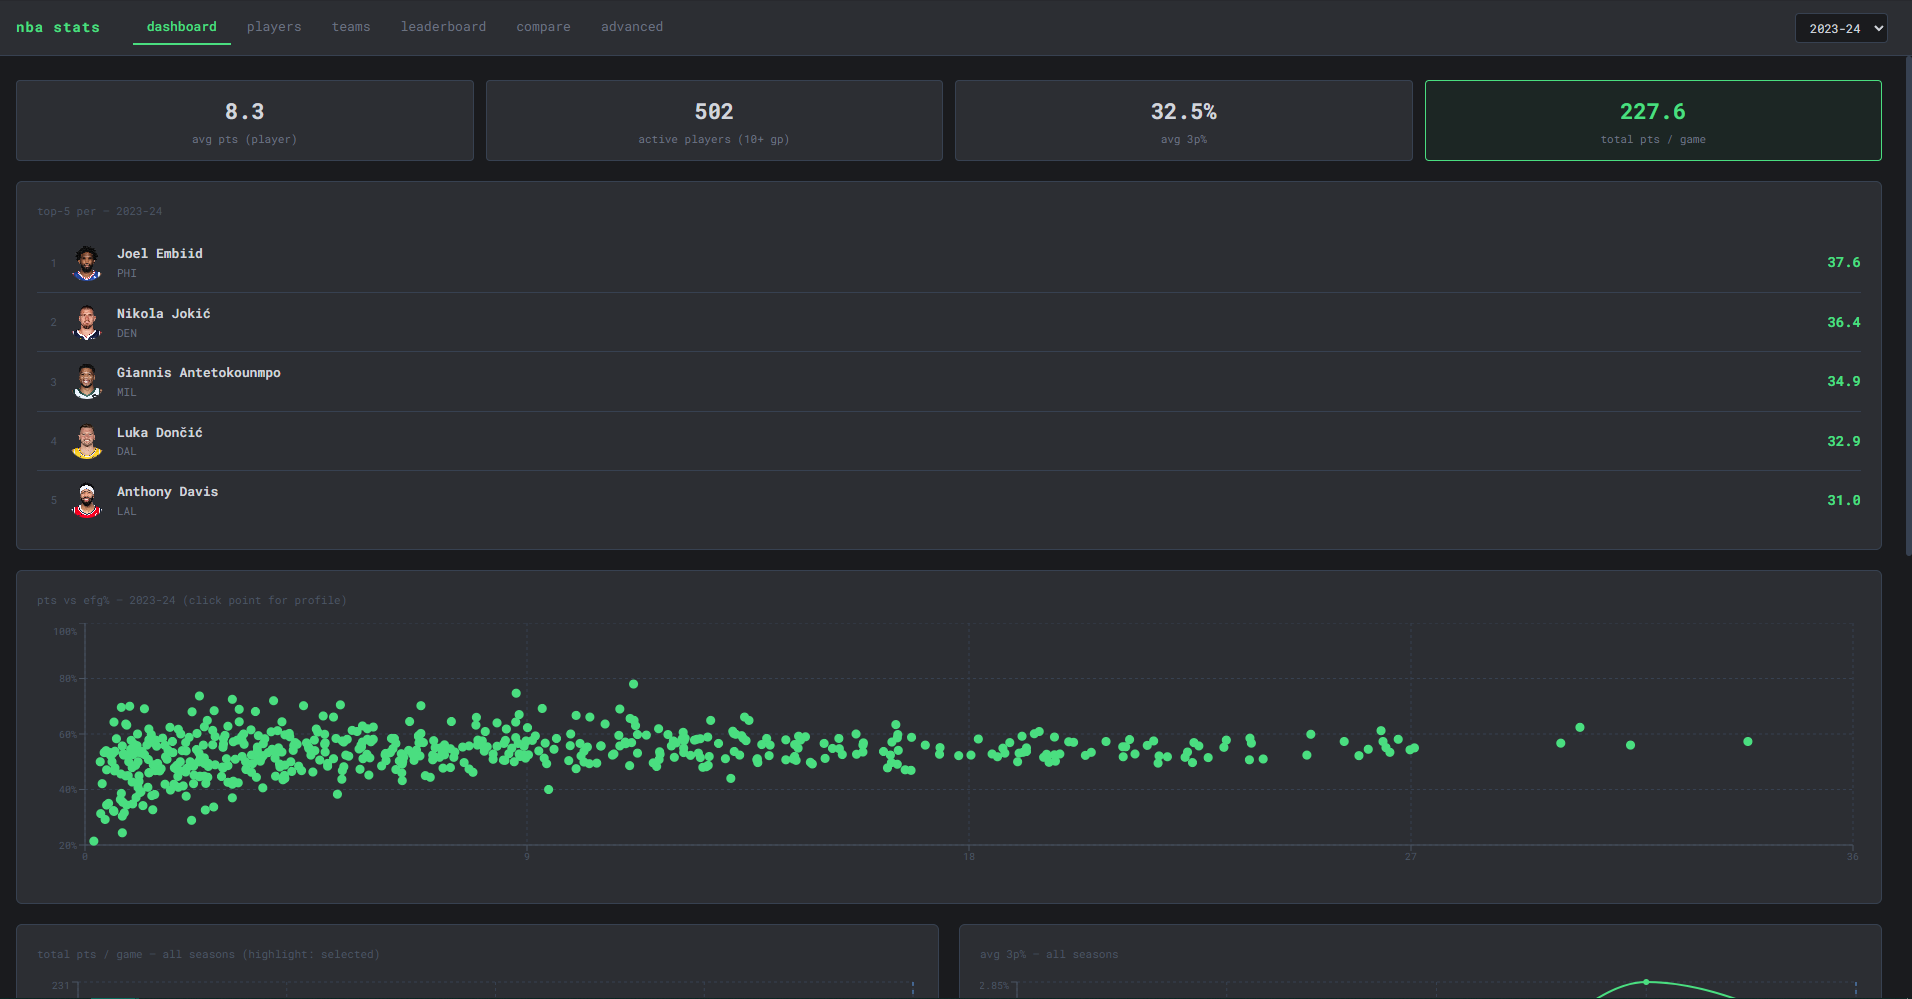
\includegraphics[width=\textwidth]{../img/dash.png}
\caption{Главная страница приложения (Dashboard)}
\label{fig:ui-dashboard}
\end{figure}

\begin{figure}[H]
\centering
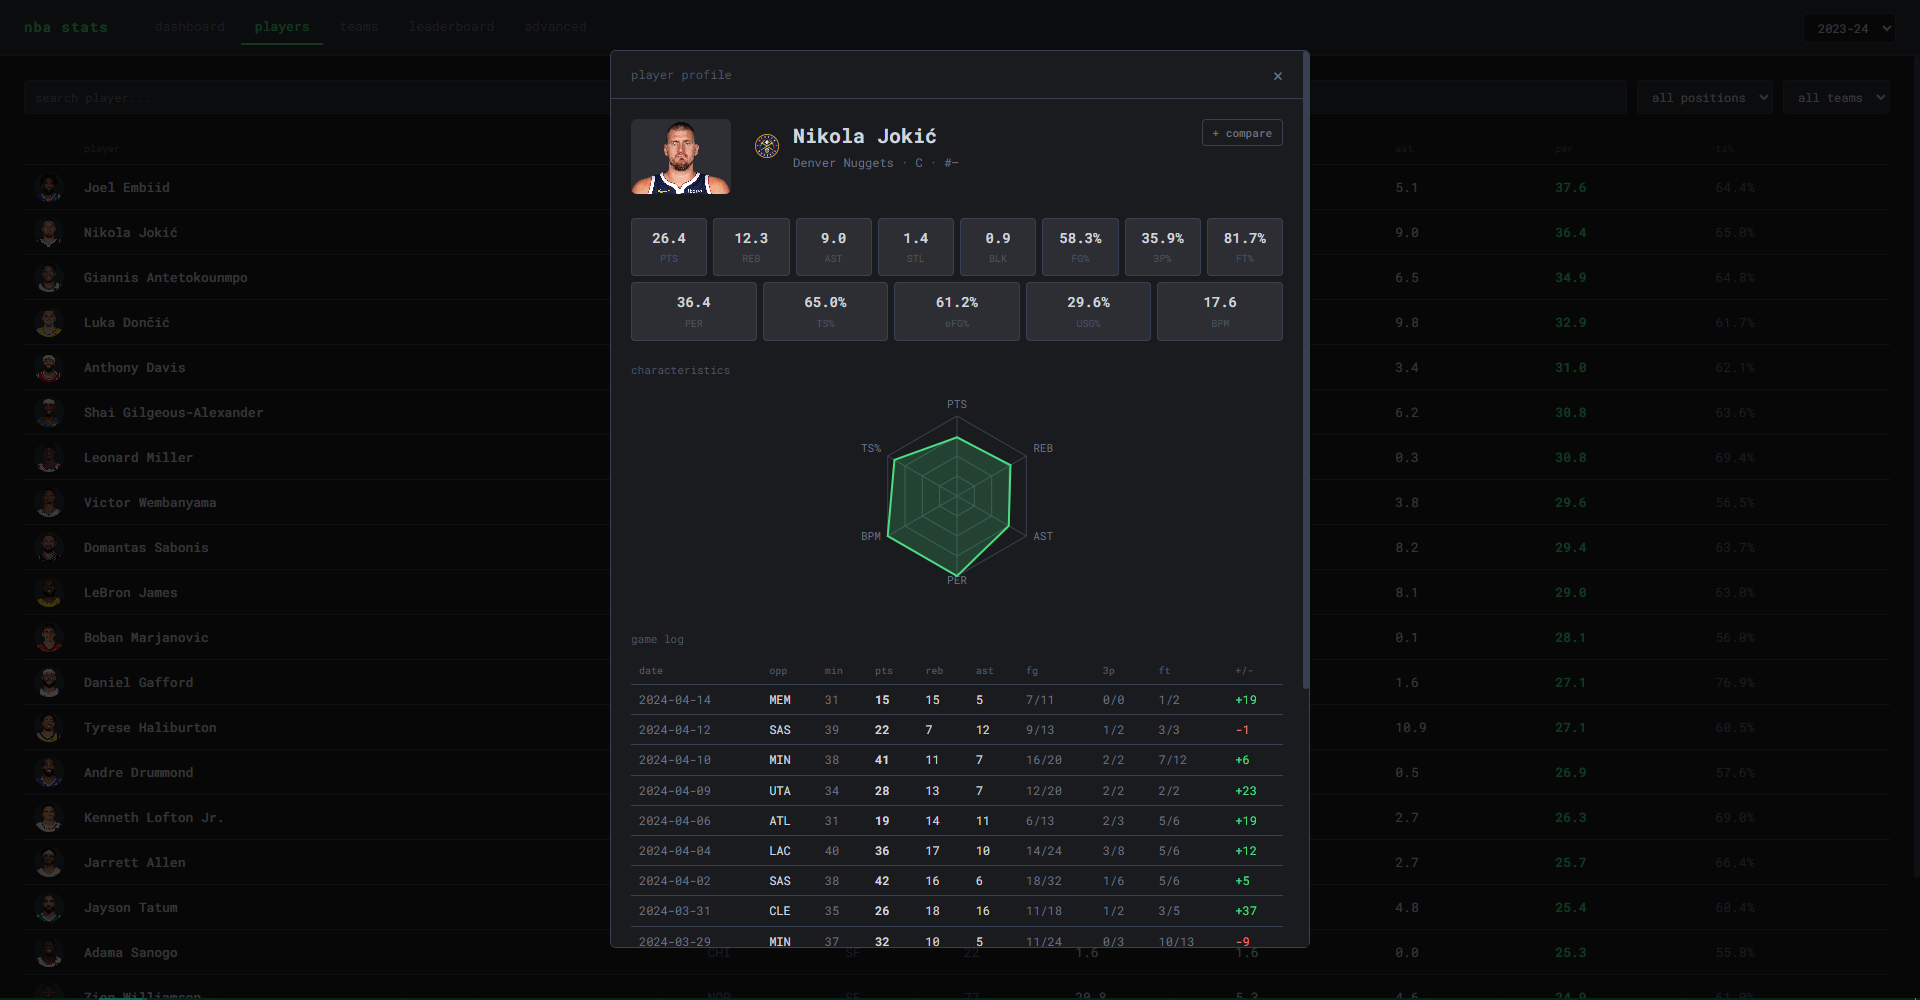
\includegraphics[width=\textwidth]{../img/player.png}
\caption{Модальное окно профиля игрока: сезонные метрики и игровой журнал}
\label{fig:ui-modal}
\end{figure}

\begin{figure}[H]
\centering
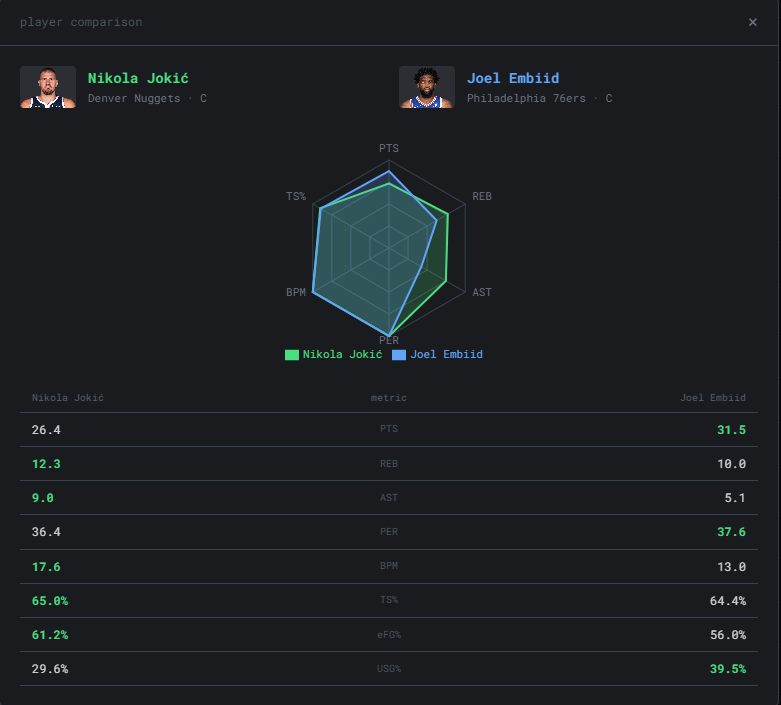
\includegraphics[width=0.8\textwidth]{../img/comp.png}
\caption{Модальное окно сравнения профилей двух игроков}
\label{fig:ui-compare}
\end{figure}


\section*{Приложение Е. Презентация}
\addcontentsline{toc}{section}{Приложение Е. Презентация}

\noindent презентация



\end{document}
